\documentclass[a4paper,oneside,12pt]{report}

%------------ package pour langue fr ------
\usepackage[utf8]{inputenc}
\usepackage[french]{babel}
\usepackage[T1]{fontenc}
\usepackage{multicol}
\usepackage{enumitem}
\usepackage{multirow}
\setcounter{secnumdepth}{5} 
%------------- for embedding images----------
\usepackage{graphicx} 
\usepackage{float}
\usepackage[export]{adjustbox}
\usepackage{amsfonts,epsfig,epstopdf,titling,url,array}
\usepackage{lscape}

\usepackage{amsmath}
\usepackage{amssymb}
\usepackage{amsthm}
%--------- pour le style de la page ----------
\usepackage[top=2.5cm, bottom=2.5cm, left=2.5cm, right=2.5cm]{geometry}

\usepackage[]{geometry}


\usepackage[french,ruled,vlined]{algorithm2e}
\usepackage[noend]{algorithmic}

%%% francisation des algorithmes 
\renewcommand{\algorithmicrequire} {\textbf{\textsc{Entrées:}}} \renewcommand{\algorithmicensure} {\textbf{\textsc{Sorties:}}} \renewcommand{\algorithmicwhile} {\textbf{tantque}} 
\renewcommand{\algorithmicdo} {\textbf{faire}} 
\renewcommand{\algorithmicendwhile}{\textbf{fin tantque}} \renewcommand{\algorithmicend} {\textbf{fin}} 
\renewcommand{\algorithmicif} {\textbf{si}} 
\renewcommand{\algorithmicendif} {\textbf{finsi}} 
\renewcommand{\algorithmicelse} {\textbf{sinon}} 
\renewcommand{\algorithmicthen} {\textbf{alors}} 
\renewcommand{\algorithmicfor} {\textbf{pour}} 
\renewcommand{\algorithmicforall} {\textbf{pour tout}}
\renewcommand{\algorithmicdo} {\textbf{faire}} 
\renewcommand{\algorithmicendfor} {\textbf{fin pour}} \renewcommand{\algorithmicloop} {\textbf{boucler}} \renewcommand{\algorithmicendloop} {\textbf{fin boucle}} \renewcommand{\algorithmicrepeat} {\textbf{répéter}} \renewcommand{\algorithmicuntil} {\textbf{jusqu'à}}
\renewcommand{\algorithmicreturn} {\textbf{Retourner}}
\renewcommand{\algorithmiccomment}[1]{\hfill$\blacktriangleright$ #1}



\usepackage{setspace}
\setstretch{1,15}
\usepackage{txfonts} %//pour utiliser times new roman dans le document
\usepackage{fancyhdr}
\fancyhf{} % clear all header and footers
\renewcommand{\headrulewidth}{0pt} % remove the header rule
\fancyfoot[RE,RO]{\thepage} % Left side on Even pages; Right side on Odd pages
\pagestyle{fancy}	
\fancypagestyle{plain}{%
  \fancyhf{}%
  \renewcommand{\headrulewidth}{0pt}%
  \fancyhf[lef,rof]{\thepage}%
}
\renewcommand{\headrulewidth}{0.4pt}
\lhead{\textbf{Chapitre \thechapter}}
\fancyhead[R]{\rightmark}
%--------------------------- Sommaire ----------------------------%
\usepackage{hyperref}
\usepackage{amssymb}
\usepackage{natbib}
\theoremstyle{definition}
		\newtheorem{defn}{Definition}[section]
		\newtheorem{conj}{Conjecture}[section]
		\newtheorem{exmp}{Example}[section]
\usepackage[table,dvipsnames]{xcolor}	

\usepackage{pifont}% http://ctan.org/pkg/pifont
\newcommand{\xmark}{\color{red}\ding{55}}%
\newcommand{\cmark}{\color{PineGreen}\ding{51}}	
\usepackage[T1]{fontenc}
\newcolumntype{R}[1]{>{\raggedleft\arraybackslash }b{#1}}
\newcolumntype{L}[1]{>{\raggedright\arraybackslash }b{#1}}
\newcolumntype{C}[1]{>{\centering\arraybackslash }b{#1}}
%\usepackage{arabtex}
\usepackage[most]{tcolorbox}


\tcbset{
    frame code={}
    center title,
    left=0pt,
    right=0pt,
    top=0pt,
    bottom=0pt,
    colback=gray!70,
    colframe=white,
    width=\dimexpr\textwidth\relax,
    enlarge left by=0mm,
    boxsep=5pt,
    arc=0pt,outer arc=0pt,
    }
% Load the package with the acronym option
\usepackage[acronym]{glossaries}
\usepackage{appendix}
%\usepackage{setspace}
\usepackage{subfig}
 
 
 
 
% Generate the glossary
\makeglossaries
\usepackage{pdfpages} 
\begin{document}

%Page de garde (page de titre)							Obligatoire
\pagenumbering{Roman}
\begin{titlepage}

\newgeometry{top=0mm,right=20mm,left=20mm,bottom=0mm}



	%--------------------  Entete de l'Ecole ----------------------%

	\begin{figure}[t]
		
\includegraphics[scale=0.75]{./ressources/image/ESI.png}\\[0.6in]
	\end{figure}
	
	
	
	%--------------------------------------------------------------%
	\begin{center}
	
	%------------------------  Le sujet ---------------------------%
		\LARGE \textbf{ Mémoire}\\
		\Large{
			Pour Obtention du diplôme d'ingénieur En Informatique\\
			\textbf{Option : Système Informatique (SIQ)}
			%\textsc thèse D'Ingéniorat En Informatique sous le thème :
		}\\[0.2in]
		\huge {
		\rule{\linewidth}{.5pt}
			\textbf{
				Étude et implémentation des méthodes de compression de graphe par extraction de motifs et k2-trees
			} 
			\rule{\linewidth}{.5pt}
		}\\[0.5in]
		\Large
	%--------------------------------------------------------------%	
	
	%-------------------------  Mon nom ---------------------------%
	\textbf{Réalisé par:}\\
	\begin{multicols}{2}
			\Large 	Mlle. Hafsa Bousbiat\\
			\large eh\_bousbiat@esi.dz\\
			ESI\\
		\columnbreak
 			\Large Mlle. Sana Ihadadene\\
			\large es\_ihadadene@esi.dz\\
			ESI \\
		
	\end{multicols} 
	
	\vskip 0.1in
	%--------------------------------------------------------------%	

	%-----------------------  Encadreures -------------------------%
	 \textbf{Encadré par:}\\
	 
	 \begin{multicols}{2}
			\Large 	Dr. Karima Amrouche\\
			\large k\_amrouche@esi.dz\\
			ESI\\
		\columnbreak
 			\Large Dr. Hamida Seba\\
			\large hamida.seba@univ-lyon1.fr\\
			Université de Lyon \\
	\end{multicols}
	
	%--------------------------------------------------------------%	
	
	\small
	\vskip 0.3in
	Octobre 2018 \\
	Année Universitaire: 2018-2019\\
	
	\end{center}		
\restoregeometry
\end{titlepage}

%Remerciements											Obligatoire
\begin{center}
	\par
	\textit{
		\vskip 1in
		\Huge 
			Remerciement \\[0.5in]
			\addcontentsline{toc}{chapter}{\numberline{}Remerciement}
	}
\end{center}
	\par
  Nous tenons d'abord à exprimer notre gratitude à l'égard de nos encadrants, Madame Seba
Hamida, Madame Amrouche Karima et Monsieur Mohammed pour leur précieuse	aide, leur judicieux conseils  et pour le temps qu'ils nous ont consacré tout au long de ce PFE.\\


Nous remercions également toute l'équipe pédagogique de l'École Nationale
Supérieure d'Informatique, et à leur tète les enseignants pour la richesse et la qualité de la formation qu'ils nous ont offert tout au long de notre cursus.\\


Nous tenons à remercier les membres du jury qui nous ont fait l’honneur d’accepter de juger
cet humble travail.\\


Enfin, nous adressons nos plus sincères remerciements à tous nos proches et amis, qui nous ont toujours encouragée au cours de la réalisation de ce mémoire.
Merci à tous et à toutes.

\newpage
 


%Résumé												Obligatoire

\thispagestyle{plain}
\begin{center}
	\par
	\textbf{
		\vskip 0.5in
		\LARGE 
			Résumé \\[0.15in]
			\addcontentsline{toc}{chapter}{\numberline{}Résumé}
	}
\end{center}
	\par
    
    Nous vivons dans un monde où la quantité d'informations ne cesse d'augmenter et dont la bonne gestion implique l'utilisation des graphes qui se sont répandus dans différents domaines allant des réseaux sociaux et de communication jusqu'aux domaines de la chimie et de la biologie. 	Cette abondance de données générées fait appel à une technique aussi vieille que la discipline de traitement de données mais qui connait de nouveaux défis aujourd'hui : la compression. La compression de graphes est un domaine dans lequel le graphe initial subit des transformations pour en obtenir une version plus réduite et compacte permettant, dans la majorité des cas, d'effectuer les traitements dans un temps nettement meilleur.\\

 Ce mémoire de fin d'études traitent deux classes de méthodes de compression de graphes: les méthodes basées sur les arbres k2-trees et les méthodes basées sur l'extraction de motifs. Nous proposons, en premier lieu, d'enrichir un projet entamé dans un PFE précédent. Nous établirons pour cela deux moteurs de compression : $k^2$-GraCE pour $k^2$-trees Graph Compression Engine et P-GraCE pour Pattern Graph Compression Engine. En second temps, nous proposons de généraliser un schéma existant de compression par extraction de motifs pour le cas des graphes dynamiques tout en l'hybridant avec une méthode $k^2$-Trees afin de tirer profit de ses performances. Cette proposition est motivé par le caractère évolutif de la majorité des situation modélisées par les graphes.\\
 
 Nous nous concentrerons  à la fin de ce travail sur l'évaluation des méthodes des deux moteurs en utilisant des benchmarks de graphes réels de domaines hétérogènes. Pour mener à bien cette dernière étapes, nous utiliserons deux métriques : le taux de compression et le nombre de bits par liens (bpe pour bits per edge).\\\\\textbf{Mots Clés :} \textit{Compression de graphes, Big Data, Extraction de motifs, K2-trees, Graphe du Web.}
 
\newpage
\thispagestyle{plain}
\begin{center}
	\par
	\textbf{
		\vskip 0.5in
		\LARGE 
			Abstract \\[0.15in]
	}
\end{center}
	\par
    
    We live in a world where the amount of information is constantly increasing and whose good management involves the use of graphs that have spread in different fields from social and communication networks to the fields of chemistry and biology. This abundance of generated data calls for a technique that is as old as the discipline of data processing but which is facing new challenges today: compression. Graph compression is a field in which the initial graph undergoes transformations in order to obtain a smaller and more compact version allowing, in the majority of cases, to perform the processings in a much better time.\\

 This dissertation deals with two classes of graph compression methods: the k2-trees methods and the methods based on pattern extraction. In the first place, we propose to extend and enrich a project started in a previous work. In order to accomplish this, we propose two compression engines: $k^2$-GraCE for $k^2$-trees Graph Compression Engine and P-GraCE for Pattern Graph Compression Engine. Secondly, we propose to generalize an existing pattern extraction compression scheme for the case of dynamic graphs while hybridizing it with a $k^2$-Trees method in order to take advantage of its performance. This proposition is motivated by the evolutionary nature of the majority of situations modeled by graphs.\\
 
 We will focus at the end of this work on evaluating the methods of the two engines using benchmarks of real graphs from heterogeneous domains. To objectively carry out this last step , we will use two metrics: the compression ratio and the number of bits per link (bpe). \\\\\textbf{Key words :} \textit{Graph compression, Big Data, Pattern extraction, K2-trees, Web graph.}

\newpage
 
 %%% Manque resume en arabe 


 
\includepdf[page=-]{psq_absract_ar}

%Sommaire (Table des matières)							Obligatoire
\pagestyle{plain}
\tableofcontents
\newpage



%Liste des figures										Selon besoin
\listoffigures
\addcontentsline{toc}{chapter}{\numberline{}Liste des figures}
\cleardoublepage

%Liste des tableaux										Selon besoin

\listoftables
\addcontentsline{toc}{chapter}{\numberline{}Liste des tableaux}
%\cleardoublepage



\printglossaries



\cleardoublepage

%Introduction (début de la pagination)					bligatoire

\pagenumbering{arabic}

	\thispagestyle{plain}
		\Huge{ 
			\textbf {Introduction générale}} \\[0.5in]
			\addcontentsline{toc}{chapter}{\numberline{}Introduction générale}
			\normalsize
			Avec l'énorme quantité de données produites par les activités humaines de nos jours, le problème de données massives (Big data) est devenu un enjeu essentiel. Un des outils les plus efficaces pour structurer et manipuler ces données est l'utilisation des graphes. Les graphes sont des outils de modélisation utilisés dans beaucoup de domaines pour la représentation des données : réseaux sociaux et de communication (entités reliées entre elles par des liens physiques ou communautaires), chimie (relations entre les atomes), biologie (interactions entre protéines par exemple) et bien d'autres domaines.\\
			
	Face à cette infobésité, les algorithmes classiques de traitement et de gestion des données se montrent incapables d'offrir des réponses dans un temps raisonnable. Plusieurs solutions ont été pensées pour contrer ce volume de données. Une des solutions les plus anciennes mais qui connait de nouveaux défis de nos jours est la \textit{ compression de données}.\\

	Le domaine de compression de données est une branche de la théorie de l'information qui s'intéresse à minimiser la taille des données à stocker, traiter et transmettre améliorant ainsi de façon directe les temps de traitement. Parallèlement à cela, nous trouvons la compression des graphes qui est un domaine dans lequel le graphe initial subit des transformations pour en obtenir une version plus réduite. Différentes techniques, basées sur différentes approches, permettent cette compression, avec ou sans perte d'information, et génèrent de nouveaux graphes sur lesquels il est beaucoup plus intéressant d'effectuer les différents traitements.\\ 

Cependant, deux types de méthodes de compression de graphes se sont distinguées parmi tout les autres types de méthodes : les méthodes de compression en utilisant les arbres k2-trees et les méthodes de compression par extraction de motifs. En effet, elles permettent de trouver dans la majorité des cas un bon compromis entre l'espace mémoire et les temps de traitement. Ces deux classes de méthodes feront l'objet de notre étude.\\
		
			Notre première contribution  portera sur la conception, l'implémentation et l'évaluation de 	deux moteurs de compression, 
		\newacronym{$k^2$-GraCE}{$k^2$-GraCE}{$k^2$-trees Graph Compression engine (Moteur de compression des graphes par les arbres $k^2$-trees )}	
		\newacronym{P-GraCE}{P-GraCE}{Pattern Graph Compression engine (Moteur de compression des graphes par extraction de motifs)}			
			\gls{$k^2$-GraCE} 
			 et \gls{P-GraCE}, chacun englobant les méthodes relatives à une classe. Nous visons à travers cela à comparer entre les performances des méthodes s'intégrant dans ces deux classes. Notre deuxième contribution consiste en la proposition d'une nouvelle méthode de compression pour les graphes dynamiques, s'intitulant 
			 \newacronym{ddsm}{DDSM}{Dynamic Dense Subgraph Mining (Compression de graphe sous-graphes denses dynamiques) }
			 \gls{ddsm}. \\
			
			
			 Nous avons hiérarchisé notre mémoire en cinq grands chapitres. Le premier est une introduction au domaine de la théorie des graphes. Dans le second chapitre, nous introduisons les définitions de base du domaine de compression de données appliqué aux graphes ainsi que les différentes méthodes de compression existantes sous forme d'une classification que nous proposons. Par la suite, dans le troisième chapitre , nous détaillons la conception de nos deux moteurs de compression de graphes et nous décrirons les bases théoriques de notre méthode, puis nous donnons dans le quatrième chapitre  les détails de l'implémentation que nous proposons. Finalement, nous présentons dans le dernier chapitre les différents tests de performance et les résultats obtenus.
	
	\cleardoublepage
\pagestyle{fancy}
\fancypagestyle{plain}{%
  \fancyhf{}%
  \renewcommand{\headrulewidth}{0pt}%
  \fancyhf[lef,rof]{\thepage}%
}
\renewcommand{\headrulewidth}{0.4pt}
\lhead{\textbf{Chapitre \thechapter}}
\fancyhead[R]{\rightmark}

\part{Synthèse bibliographique}
%---->chapitre 01 :« cadrage du projet »
	\chapter{ Théorie des graphes}
	%%Ajouter une petite introduction pour ce chapitre
	  Pour faciliter la compréhension d'un problème, nous avons tendance à le dessiner ce qui nous amène parfois même à le résoudre. La théorie des graphes est fondée à l'origine sur ce principe.  Historiquement, elle représente un domaine mathématique qui s'est développé  au sein d'autres disciplines comme la chimie, la biologie, ... Elle constitue aujourd'hui un corpus de connaissances très important et un instrument efficace pour résoudre une multitude de problèmes.

Dans ce chapitre, nous présenterons les notions et les concepts clés relatifs aux graphes , à savoir : la définition d'un graphe, ses types et sa représentation structurelle. Nous clôturons le chapitre avec quelques domaines d'application des graphes.

	
	\section{Graphe non orienté}
			\subsection{Définitions et généralités}
		
Un graphe non orienté G est la donnée d’un couple (V , E) où V = \{$ \textit{v}_{1} , \textit{v}_{2} ,..., \textit{v}_{n} $\} est un ensemble fini dont les éléments sont appelés sommets ou nœuds ( Vertices en anglais ) et  E=\{$\textit{e}_{1} ,  \textit{e}_{2} ,…, \textit{e}_{m} $\} est un ensemble fini d'arêtes ( Edges en anglais ). Toute arête \textit{e} de E correspond à un couple non ordonné de sommets ( $\textit{v}_{i} , \textit{v}_{j}$ ) $\in$ E $\subset$  $V \times V$ représentant ses extrémités \citep{muller} \citep{fages2014exploitation}.
\\Soient \textit{e} = ($\textit{v}_{i} , \textit{v}_{j}$) et \textit{e'}=($\textit{v}_{k} , \textit{v}_{l}$) deux arêtes de E, On dit que :
\begin{itemize}
\item $\textit{v}_{i}$ et $\textit{v}_{j}$ sont les extrémités de \textit{e} et \textit{e} est incidente à $\textit{v}_{i}$ et $\textit{v}_{j}$ \citep{hennecart2012elements}.
\item $\textit{v}_{i}$ et $\textit{v}_{j}$ sont voisins ou adjacents, s'il y a au moins une arête entre eux dans E \citep{IUTLyonInformatique}.
\item L'ensemble des sommets adjacents aux deux extrémités de \textit{e} est appelé le voisinage de \textit{e} \citep{muller}. 
\item \textit{e} et \textit{e'} sont voisins s'ils ont une extrémité commune  \citep{lopez2003cours}.
\item L'arête \textit{e} est une boucle si ses extrémités coïncident, i.e, $\textit{v}_{i}$ = $\textit{v}_{j}$ \citep{IUTLyonInformatique}. 
\item L'arête \textit{e} est multiple si elle a plus d'une seule occurrence dans l'ensemble E.
\end{itemize}	
		 
\subsection{Représentation graphique}
Un graphe non orienté G peut être représenté par un dessin sur un plan comme suit \citep{muller}:

\begin{itemize}
\item Les nœuds $\textit{v}_{i}$ $\in$ V de G sont représentés par des points distincts.
\item 	Les arêtes \textit{e} = ($\textit{v}_{i}$,$\textit{v}_{j}$) $\in$ E de G sont représentés par des lignes, pas forcement rectilignes, qui relient les extrémités de chaque arête \textit{e}.
\end{itemize}

%% L'exemple de la représentation graphique 
\textbf{Exemple :}
 Soit g=(V1 , E1) un graphe non orienté tel que : V1=\{ 1,2,3,4,5 \} et E1=\{(1,2), (1,4), (2,2), (2,3), (2,5), (3,4)\}.
La représentation graphique de g est alors donnée par le schéma de la figure \ref{graphNonOriente}.
\\
\begin{figure}[H]
\begin{center}
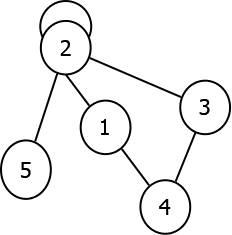
\includegraphics[height=120 pt, width=130 pt]{./ressources/image/graphNonOriente.png} 
\end{center}
\caption{Exemple de représentation graphique d'un graphe non orienté}
\label{graphNonOriente}
\end{figure}

		\subsection{Propriétés d'un graphe}
		
		\begin{itemize}[label=$\circ$]
			
			\item \textbf{Ordre d'un graphe:} On appelle ordre d’un 					graphe le nombre de ses sommets, i.e, Card(V) \citep{DUT}.
			
			\item  \textbf{Taille d'un graphe:} On appelle taille d’un 				graphe le nombre de ses arêtes, i.e, Card(E) \citep{DUT}.
			
			\item  \textbf{Degré dans un graphe:}
			
			
			\begin{itemize}[label=$\bullet$]
				\item \textbf{Degré d'un sommet : } Le degré d’un sommet noté \textit{d}($\textit{v}_{i}$) est le nombre d'arêtes incidentes à ce sommet, sachant qu’une boucle compte pour deux \citep{muller}. Dans l'exemple de la figure \ref{graphNonOriente}, le degré du sommet (1) est : \textit{d}(1)=2.
				
				\item \textbf{Degré d'un graphe : }Le degré d’un graphe est le degré maximum de ses sommets, i.e, max(\textit{d}($\textit{v}_{i}$)) \citep{muller}. Dans l’exemple de 				la figure \ref{graphNonOriente}, le degré du graphe g est \textit{d}(2)=5.
			\end{itemize}
			
			\item \textbf{Rayon et diamètre dans un graphe:}
			\begin{itemize}[label=$\bullet$]
				\item \textbf{Distance : }La distance entre deux sommets 	\textit{v} et \textit{u} est le plus petit nombre d’arêtes qu’on doit parcourir pour aller de \textit{v} à \textit{u} ou de \textit{u} à \textit{v} \citep{muller}. 
				
				\item 	\textbf{Diamètre d’un graphe :} C’est la plus grande 	distance entre deux sommets de ce graphe \citep{muller}. 
				
				\item 	\textbf{Rayon d’un graphe : }C’est la plus petite distance entre deux sommets de ce graphe \citep{parlebas1972centralite}. 
			\end{itemize}
		\end{itemize}
		
	
			
	
			
	\section{Graphe orienté}	
		
		\subsection{Définitions et généralités}
		Un graphe orienté G est la donnée d'un couple (V , E) où
		V est un ensemble fini dont les éléments sont appelés les sommets de G et 
		E  $\subset$ V x V est un ensemble de couples ordonnés de sommets dits arcs ou arêtes \citep{muller}. G est appelé dans ce cas digraphe (directed graph).\\
		 Pour tout arc e = ( $v_{i}$ , $v_{j}$) $\in$ E :
		 \begin{itemize}  
			\item $v_{i}$ est dit extrémité initiale ou origine de e et $v_{j}$ est l'extrémité finale de e \citep{muller}.
			
			\item $v_{i}$ est le prédécesseur de $v_{j}$ et $v_{j}$ est le successeur de $v_{i}$ \citep{IUTLyonInformatique}.
			
			\item les sommets $v_{i}$ , $v_{j}$ sont des sommets adjacents \citep{Pres}.
			
			\item e est dit sortant en $v_{i}$ et incident en $v_{j}$ \citep{Pres}.
			
			\item e est appelé boucle si $v_{i}$ = $v_{j}$, i.e l'extrémité initiale et finale représente le même sommet \citep{IUTLyonInformatique}.
			
		\end{itemize}
		 
		
		\subsection{Représentation graphique}
		
		
		Un graphe G = (V , E) peut être projeter sur le plan en représentant:
		\begin{itemize} 
		\item Dans un premier temps les nœuds $v_{i}$ $\in$ V par des points disjoints du plan.
		\item Et dans un second temps les arêtes e = ( $v_{i}$ , $v_{j}$) $\in$ E par des lignes orientées reliant par des flèches les deux extrémités de e. 
		\end{itemize}
		
		\textbf{Exemple:}
		
		Soit g = ($V_{1}$ , $E_{1}$) un digraphe tel que : $V_{1}$ = \{ 1,2,3,4 \} et  $E_{1}$ = \{(1,2),(1,3),(3,2),(3,4),(4,3)\}.
		
		Le représentation graphique de g est alors donné par le schéma de la figure \ref{grapheOr}.
	
		
			\begin{figure}[h]
			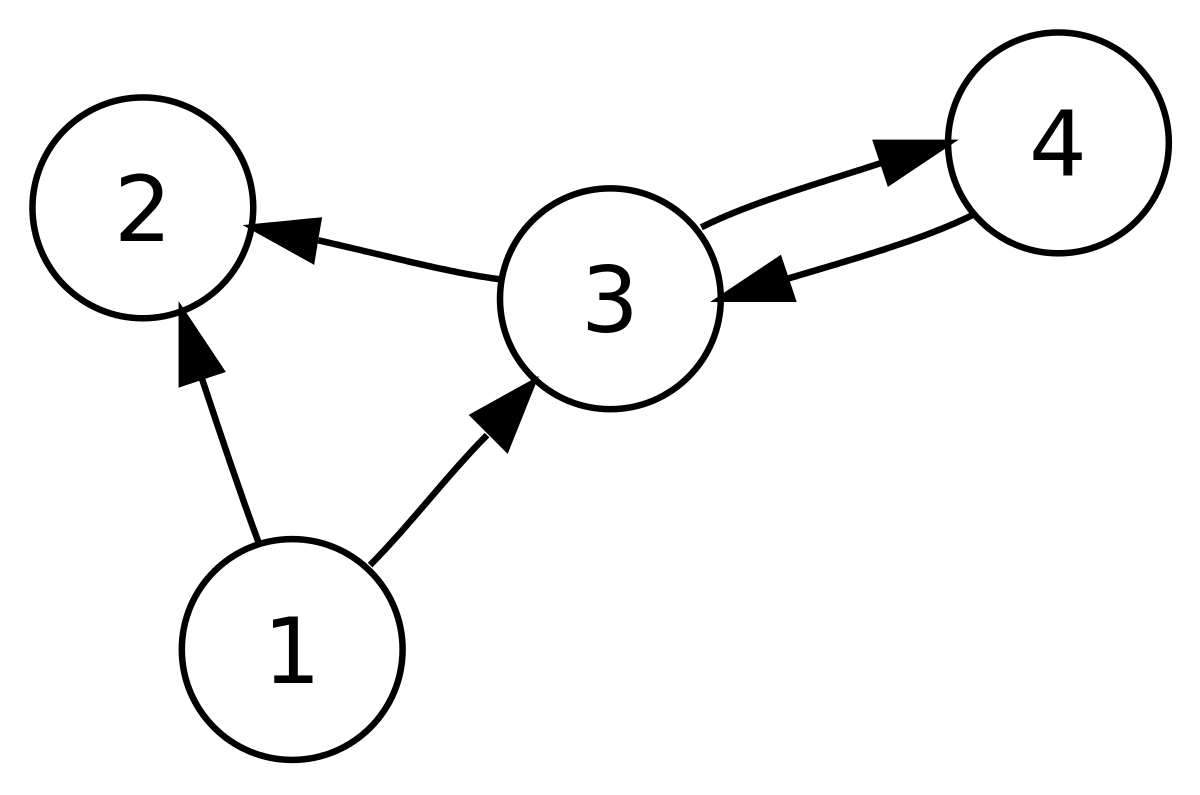
\includegraphics[scale=0.15,center]{./ressources/image/RepDiGraphe.png}
			\caption[Exemple de représentation graphique d'un digraphe.]{Exemple de représentation graphique d'un digraphe.}
			\label{grapheOr}
			\end{figure}
			
		
		\subsection{Quelques Propriétés:} %%% Arevoire 
			\begin{itemize}[label=$\circ$]
			\item\textbf{Ordre d'un digraphe:}
			est le nombre de sommets n = Card(V) \citep{DUT}.
			
			\item\textbf{taille d'un digraphe:} est le nombre d’arcs m = Card(A) \citep{DUT}.
			
			\item\textbf{Degré dans un digraphe:}
			Le degré d'un sommet $v_{i}$ $\in$ V dans un digraphe G=(V , E) est donnée par la formule :
			\begin{center}
				d($v_{i}$) = $d^+(v_{i}$) + $d^-(v_{i}$\\
			\end{center}			 
			 où $d^+(v_{i}$) est le nombre d'arcs sortants au sommet $v_{i}$ et est appelé degré extérieure et $d^-(v_{i}$) représente le nombre d'arcs incidents et est appelé degré intérieur \citep{muller}.
			 
			 \item\textbf{Voisinage dans un digraphe:}
			 Le voisinage d'un sommet $v_{i}$ $\in$ V, noté V($v_{i}$), dans un digraphe G = (V , E) est:
			 	\begin{center}
				V($v_{i}$) = succ($v_{i}$) $\bigcup$ pred($v_{i}$),
				\end{center}
				
				où succ($v_{i}$) est l'ensemble des successeurs de $v_{i}$ et pred($v_{i}$) est l'ensemble de ses prédécesseurs \citep{bac}, i.e le voisinage de $v_{i}$ est l'ensemble des sommets qui lui sont adjacents.
			
			\end{itemize}
			
		
	\section{Notion de Connexité}
	
	Les structures de graphes sont généralement exploitables à travers leurs interrogation qui permet de fournir des réponses aux problèmes modélisés. L'un des informations les plus importantes dans un graphe est la notion des relations (indirectes ou indirecte) entre deux nœuds ou plus formellement la connexité dans un graphe. Dans cette partie nous allons définir les concepts relatives à cette notion.
	
	\begin{itemize} [label = $\bullet$]
		
			 
			 \item \textbf{Chemin (resp. Chaine):}
			est une liste de sommets S= $(v_{0},v_{1},v_{2},...,v_{k})$ telle qu’il existe un arc (resp. une arête) entre chaque couple de sommets successifs.
			 
			 
			  \item \textbf{Cycle (resp. Circuit):} 
			 est un chemin (resp. chaine) dont le premier et le dernier sommet sont identiques \citep{DUT}.
			 
			 		\item \textbf{Graphe connexe:}
			Un graphe non orienté (resp. orienté) est dit connexe (resp. fortement connexe) si pour tout pair de sommets ($v_{i}$, $v_{j}$) il existe un chemin S les reliant \citep{muller}.
			 
		\end{itemize}
	
	\section{Quelques types de graphe}
		 %% classifier selon le type du graphe en entree
	Avec les avancées technologiques au fil du temps, plusieurs types de graphes ont connus le jours. En effet, La complexité et la variété des problèmes scientifiques existants modélisés par ces derniers ont poussé les chercheurs à adapter leurs structure selon le problème auquel ils font face. Durant cette section nous allons définir les principaux types existants.
	
		\begin{itemize}[label=$\circ$]
		
			\item \textbf{Graphe Complet:} Un graphe G = (V , E) est un graphe complet si tous les sommets $v_{i}$ $\in$ V sont adjacents \citep{Pres}. Il est souvent noté $K_{n}$ où n = card(V) \citep{DUT}.
				
			
			\item \textbf{Graphe étiqueté et graphe pondéré:}
			 Un graphe étiqueté G = (V , E , W) est un graphe, qui peut être orienté ou non orienté, dont chacune des arêtes $e_{i}$ $\in$ E est doté d'une étiquette $w_{i}$. Si de plus, $w_{i}$ est un nombre alors G est dit graphe pondéré (valué) \citep{DUT}.
		
			\item \textbf{Graphe simple et graphe multiple:}
			Un graphe G = (V , E) est dit simple si il ne contient pas de boucles et toute paire de sommets est reliée par au plus une arête. Dans le cas contraire, G est dit multiple \citep{IUTLyonInformatique}.
			
		
		\end{itemize}
		
	
	\section{Graphe partiel et sous-graphe:}
    		
	La quantité de données disponible aujourd'hui et sa croissance de manière exponentielle ont favorisé la décomposition des graphes en des entités plus petites afin de garantir une facilité de compréhension et d'analyse dans le but d'extraire l'information la plus pertinente. Dans cette partie, nous allons définir de manière plus formelle ce que ces entités sont, ainsi que leurs types.
	
		
		
		
		\subsection{Définitions:}
		Soient G = (V , E), $G' = (V' , E')$ et $G'' = (V'' , E'')$ trois graphes.
		\begin{itemize}[label=$\circ$]
		
			\item Le graphe $G'$ est appelé \textbf{graphe partiel} de G si : $V' = V\ et\ E' \subset$ E \citep{DUT}. En d'autres termes, un graphe partiel est obtenu en supprimant une ou plusieurs arêtes de G.
				

			\item Le graphe $G''$ est dit \textbf{sous-graphe} de G si: $V''\subset V$ et 
			 $E''\subset E \cap (V'' x V'')$ \citep{bac}, i.e, un sous-graphe est obtenu en enlevant un ou plusieurs nœuds du graphe initial ainsi que les arêtes dont ils représentent l'une des deux extrémités.
			 
		\end{itemize}
		
		\subsection{Quelques Types de sous graphes:}
		
		\begin{itemize} [label = $\bullet$]
		
		
			\item \textbf{Une Clique :} est un sous-graphe complet de G \citep{bac}.
			
			\item \textbf{Biparti :} G' est un sous-graphe biparti si il existe une partition de V' en deux sous ensembles notés $V_{1}$ et $V_{2}$, i.e V' = $V_{1} \cup V_{2}$ et $V_{1}$ $\cap$ $V_{2}$ = $\phi$, tel que E' = $V_{1}$ x $V_{2}$ \citep{bac}.
			
			\item \textbf{Étoile :}
			 est un cas particulier de sous-graphe biparti où $V_{1}$ est un ensemble contenant le sommet central (dit \textit{hub}) uniquement et $V_{2}$ contient le reste des nœuds  (dits \textit{spokes})\citep{koutra2015summarizing} .
			 
		
			 
		\end{itemize}		
	
		
	
	
    		
    	\section{Représentation Structurelle d'un graphe}	
		\input{./Chapitres/TheorieDesGraphes/structRep.tex}
	
	\section{Les domaines d'application}
		  La diversité des domaines faisant appel à la modélisation par des graphes ne cesse d'augmenter, allant des réseaux sociaux aux réseaux électriques et réseaux biologiques et arrivant jusqu'aux World Wide Web. Dans cette partie nous allons décrire trois domaines d'application les plus répandus des graphes.
	
		\subsection{Graphes des réseaux sociaux:}
		Les réseaux sociaux représentent un lieu d'échange et de rencontre entre individus (entités) et dont l'utilisation est devenue de nos jours une nécessité.  
		Pour représenter les interactions entre ces individus, nous avons généralement besoin de faire recours aux graphes où les sommets sont des individus ou des entités et les interactions entre eux sont représenté par des liens. 
		Vue la diversité des interactions sociales, la modélisation de ces réseaux  nécessite différents types de graphes: graphes non orientés pour pour les réseaux sociaux avec des relations non
orientées, graphes orientés pour représenter des relations non symétriques
comme c'est la cas dans les réseaux de confiance, graphes pondérés pour les réseaux sociaux qui contiennent différents niveaux d'intensités dans les relations, ... etc \citep{lemmouchi2012etude}.
		
		\subsection{Graphes en Bioinformatique:}
		
		La bio-informatique est un domaine qui se trouve à l'intersection des deux grands domaines celui de l'informatique et celui de la biologie. Elle a pour but d'exploiter la puissance de calcule des équipements informatiques pour effectuer des traitements sur des données moléculaires massives \citep{pellegrini2004protein}.
		
		Elle est largement utilisée pour l’analyse des séquences d’ADN et des protéines à travers leurs modélisation sous forme de graphe. A titre d'exemple, les graphes non orientés multiples sont un outil modélisation des réseaux d’interaction protéine-protéine \citep{pellegrini2004protein}, 
		le but dans ce cas est donc l'étude du fonctionnement des protéines par rapport à d'autre.
		
		\subsection{Le Graphe du web:}
		 Le graphe du Web est un graphe orienté dont les sommets sont les pages du web et les arêtes modélise l'existence d'un lien hypertexte dans une page vers une autre \citep{brisaboa2009k}. Il représente l'un des graphes les plus volumineux: en juillet 2000 déja, on estimait qu’il contenait environ 2,1 milliards de sommets et 15 milliards d’arêtes avec 7,3 millions de pages ajoutées chaque jour \citep{guillaume2002web}. De ce fait, ce graphe a toujours attiré l'attention des chercheurs. En effet, l'étude de ses caractéristiques a donné naissance à plusieurs algorithmes intéressants, notamment l'algorithme PageRank de classement des pages web qui se trouve derrière le moteur de recherche le plus connu de nos jours : Google.	
		
	
	
			
	\section{Conclusion}
Dans ce chapitre nous avons présenté les notions et les concepts généraux qui touchent à la théorie des graphes : définitions des graphes, leurs principales propriétés, leurs représentations ainsi que leurs domaines d'application.\\
Le point important qu'on a pu tirer de cette partie est que les graphes sont devenus un moyen crucial et indispensable dans la modélisation des problèmes dans plusieurs domaines. Cependant ils deviennent de plus en plus complexes et volumineux avec la grande quantité de données disponible de nos jours. De ce fait, leur stockage, visualisation et traitement sont devenus difficile. La compression de graphe est naît comme solution à ce problème. Dans le chapitre suivant nous allons présenter la compression de graphes, son rôle et ses différentes méthodes.  
	
	
	

%---->chapitre 02 :« »
	\chapter{Compression de graphes}
	La puissance des processeurs, de nos jours, augmente plus vite que les capacités de stockage ce qui engendre un déséquilibre entre le volume des données qu'il est possible de
traiter et de stocker. Dès lors, la réduction de la taille des données, plus formellement la compression de données, a été un domaine de recherche très active. 
		
		 Dans ce chapitre, nous allons tout d’abord introduire le domaine de compression des données et son application dans la théorie des graphes. Puis dans un second
temps, nous allons présenter une étude bibliographique sur les méthodes de compression existantes  et qui s'inscrivent dans l'une des deux classes de méthodes de compression: les méthodes de compression par les k2-trees et les méthodes de compression par extraction de motifs, pour finir avec une étude comparative entre elles.
	
		
		\section{Compression de données :}
		
			 La compression de données est principalement une branche de la théorie de l'information  qui traite des techniques et méthodes liées à la minimisation de la quantité de données à transmettre et à stocker.
Sa caractéristique de base est de convertir une chaîne de caractères vers un autre jeu de caractères occupant un espace mémoire le plus réduit possible tout en conservant le sens et la pertinence de l'information \citep{lelewer1987data}.

	Les techniques de compression de données sont principalement motivées par la nécessité d'améliorer l'efficacité du traitement de l'information. En effet, la compression des données en tant que moyen peut rendre l'utilisation des ressources existantes beaucoup plus efficace. 
	
	De ce fait, une large gamme d'applications usant du domaine de compression tel que le domaine des télécommunications et le domaine du multimédia est apparue offrant une panoplie d'algorithmes de compression \citep{sethi2014data}. Sans les techniques de compression, Internet, la télévision numérique, les communications mobiles et les communications vidéo, qui ne cessaient de croître, n'auraient été que des développements théoriques.
	
	%Afin de pouvoir comparer entre ces différentes méthodes de compression, plusieurs critères ont été proposés dans la littérature. Parmi les mesures utilisées on trouve:
	%\begin{itemize}
	%	\item \textbf{Le taux de compression:} représente le rapport entre la taille des données après et avant la compression.
		
		%%% donner la formule
		
		%\item \textbf{Le facteur de compression:} représente l'inverse du taux de compression.
		
		%\item \textbf{Le temps de compression:}
	%\end{itemize}
		
		\section{Compression appliquée aux graphes:}
			La compression des graphes a été proposée comme solution pour le traitement et le stockage des graphes volumineux. Elle permet de transformer un grand graphe en un autre plus petit tout en préservant ses propriétés générales et ses composants les plus importants.
Les principaux avantages de la compression sont  \citep{liu2018graph} :
\begin{itemize}

\item \textbf{La réduction de la taille des données et de l'espace de stockage :} De nos jours, les graphes représentant les bases de données, les réseaux sociaux et tous types de données numériques sont caractérisés par une croissance exponentielle de leurs volumes, ce qui rend leur stockage difficile et couteux en terme d'espace mémoire. Les techniques de compression produisent des graphes plus petits qui nécessitent moins d'espace. Cela permet aussi de réduire le nombre d'opérations d'E/S ainsi que les communications entre nœuds dans un environnement distribué et de charger le graphe en mémoire centrale.   

\item \textbf{L'exécution rapide des algorithmes de traitement et des requêtes sur les graphes :} l'exécution des différents algorithmes de traitement sur des graphes volumineux peut s'avérer couteuse en terme de temps et peut ne pas donner les résultats attendus. La compression permet d'obtenir de petits graphes qui peuvent être traités, analysés et interrogés plus efficacement et dans un temps raisonnable. 
  
\item \textbf{La Facilité d'analyse et de visualisation des graphes :} Les techniques de compression permettent de représenter les données et les structures des graphes massives d'une manière plus significative permettant ainsi leur analyse et leur visualisation contrairement au graphes d'origines qui ne peuvent même pas être chargés en mémoire.  

\item \textbf{L'élimination du bruit :} l'un des exemples les mieux illustrant cet avantage sont les grands graphes du web qui sont considérablement bruités. Ce bruit peut perturber l'analyse en faussant les résultats et en augmentant la charge de travail liée au traitement des données. La compression permet donc de filtrer le bruit et de ne mettre en évidence que les données importantes.

\end{itemize}



			
	
			\subsection{Les types de compression:}
			La compression de graphes est définie comme l'ensemble des méthodes et techniques permettant de réduire l'espace mémoire occupé par ce derniers tout en gardant la même signification que le graphe d'origine. Dès lors, deux approches se présentent: la compression avec ou sans perte, que nous allons détailler dans ce qui suit.
			
			\begin{enumerate}[label=\alph*)]
			\item \subsubsection{Compression Sans Perte:}
			Certains domaines d'application de la compression nécessitent un niveau élevé d'exactitude et une restitution exacte, donc une compression sans perte. Dans cette catégorie, le graphe G subit des transformations pour avoir une représentation compacte $G'$ qui lors de la décompression donne exactement G. La figure ci-dessous illustre cette définition. 
			
			\begin{figure}[h]
			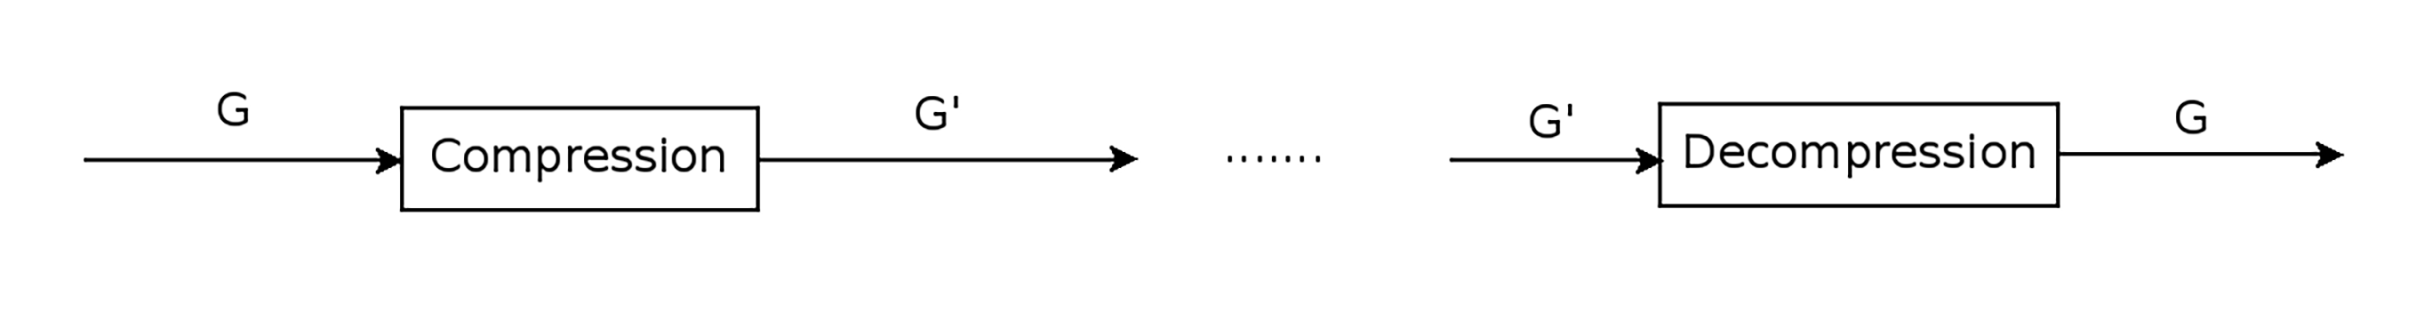
\includegraphics[scale=0.15,center]{./ressources/image/SansPerte.png}
			\caption[Compression sans perte.]{Compression sans perte.}
			\end{figure}
			
			%% citee qlq exemple de compression sans pertes
			
			\item \subsubsection{Compression Avec Perte:}
			Contrairement à la compression sans perte, la compression avec perte permet la suppression permanente de certaines informations jugées inutiles (redondantes) pour améliorer la qualité de la compression.  En d'autres termes, le graphe G subit des transformations pour avoir une représentation compacte $G'$ qui lors de la décompression donne un graphe $G''$ probablement différent de G mais l'approximant le plus possible. La figure ci-dessous illustre cette définition.   
			
			\begin{figure}[h]
			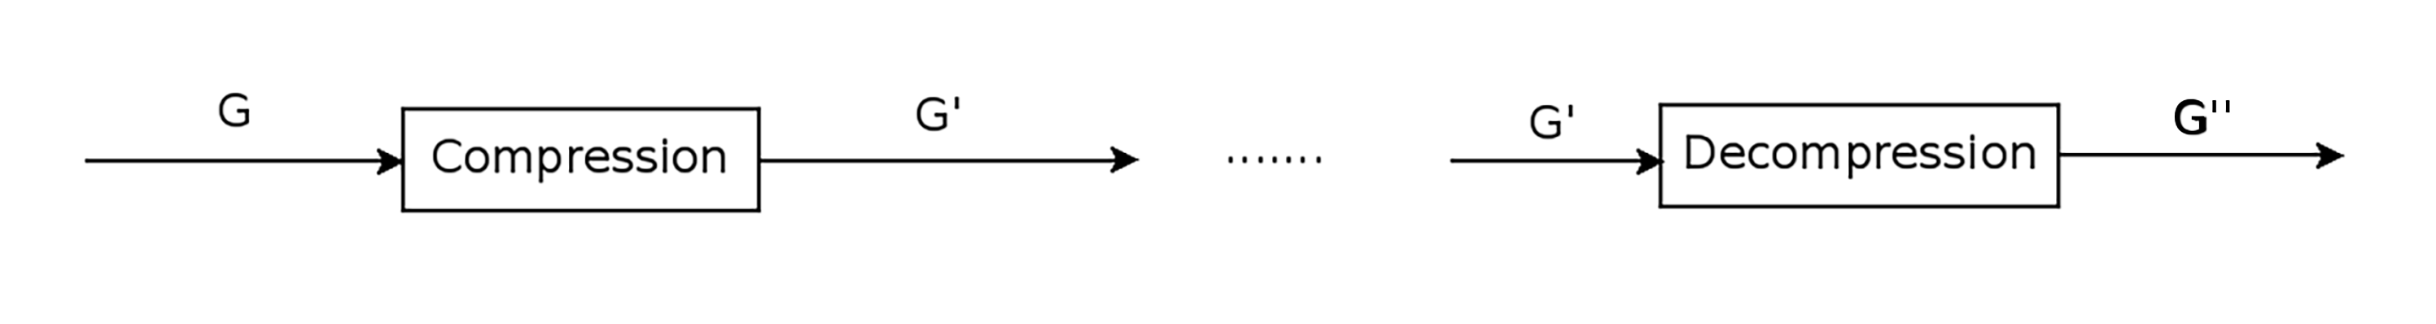
\includegraphics[scale=0.15,center]{./ressources/image/AvecPerte.png}
			\caption[Compression avec perte.]{Compression avec perte.}
			\end{figure}
			
			%%% citee qlq exemple de compression avec perte
				\end{enumerate}
			
			
			
			
	
			\subsection{Les métriques d'évaluation des algorithmes de compression:}
					
				Devant la panoplie d'algorithmes et de techniques de compression de graphe disponibles dans la littérature, des critères de comparaison  et d'évaluation entre ces méthodes doivent être bien définis. Dans cette partie, nous présenterons les principales mesures de performances.
				
				\begin{enumerate}[label=\alph*)]
					\item \subsubsection{Le temps de compression:}
				C'est une métrique qui donne le temps d'exécution de l'algorithme de compression. Elle est généralement mesurée en secondes (ou ms).
				
				%\newacronym{cr}{CR}{Ratio de compression}
				\item 	\subsubsection{Le ratio de compression:}
				Le ratio de compression (CR) est la mesure la plus courante pour calculer l'efficacité d'un algorithme de compression. Il est défini comme le rapport entre le nombre total de bits requis pour stocker les données non compressées et le nombre total de bits nécessaires pour stocker les données compressées.
				%la formule
				\begin{center}
				$
				CR = \frac{Nbre.\ de\ bits\ du\ graphe\ originale}{Nbre.\ de\ bits\ du\ graphe\ finale }
				$
				\end{center}
				
				
				Le CR est parfois appelé bit par bit (bpb) et il est défini alors comme étant le nombre moyen de bits requis pour stocker les données compressées \citep{uthayakumar2018survey}. Dans le cas des algorithmes de compression de graphe on a:
				\begin{itemize}
					\item \textbf{Le nombre de bits par nœud:}
					représente l'espace mémoire nécessaire pour stocker un nœud (bpn pour << \textit{bits per node} >> en Anglais).
					%% la formule
					
					\item \textbf{Le nombre de bits par lien:}
					représente l'espace mémoire nécessaire pour stocker un arc dans le cas d'un graphe orienté ou une arête dans le cas d'un graphe non orienté (bpe pour << \textit{bits per edge} >> en Anglais).
					%%la formule 
				\end{itemize}
				
				\item 	\subsubsection{Le taux de compression:}
				Exprimée en pourcentage, cette métrique permet de mesurer la performance de la méthode de compression. Elle peut être exprimée de deux manières différentes:
				
				\begin{itemize}
					\item \textbf{Le taux de compression:} Le rapport entre volume du graphe après compression et le volume initial du graphe.
					\begin{center}
				$
				t = \frac{La\ taille\ du\ graphe\ finale}{La\ taille\ du\ graphe\ originale }
				$
				\end{center}
					\item \textbf{Le gain d'espace: }Le gain d'espace représente la réduction de la taille du graphe compressé par rapport à la taille du graphe original.
					
					\begin{center}
				$
				G = 1 - \frac{La\ taille\ du\ graphe\ finale}{La\ taille\ du\ graphe\ originale }
				$
				\end{center}
					
					
				\end{itemize}
				%\subsubsection{L'erreur quadratique:}
				\end{enumerate}
				
				
				
				
				
				
				
				
				
			
			
			\subsection{Classification des méthodes de compression:}
				Le domaine de compression des graphes est un domaine qui a connu une grande évolution vu son importance. Une multitude de méthodes ont été proposées au cours des dernières années. Elles diffèrent l'une de l'autre dans plusieurs points : le type de graphe en entrée, le type de structure en sortie, le type de compression et la technique utilisée pour la compression. En se basant sur ces différences, plusieurs classifications ont été suggérées. Nous allons dans ce qui suit présenter les plus importantes parmi ces classifications.\\

Dans \citep{maneth2015survey}, les auteurs proposent une classification basée tout d'abord sur le type de compression. Ils regroupent les méthodes en deux catégories principales : les méthodes de compression sans perte et les méthodes de compression avec perte. La première catégorie est subdivisée à son tour selon le type de représentation du graphe en sortie : représentation succinte, représentation structurelle ou une représentation sous forme de fichier RDF\newacronym{rdf}{RDF}{Resource Description Framework}\footnote{\gls{rdf} : est un modèle de graphe destiné à décrire de façon formelle les ressources Web et leurs métadonnées, de façon à permettre le traitement automatique de telles descriptions.}. 
Les méthodes donnant une représentation succincte représentent le graphe sous forme d'une chaine de bits succincte irréversible. La sortie de ces méthodes est ainsi une structure compacte du graphe original. Parmi les méthodes de cette classe, nous trouvons : Web Framework de Boldi et Vigna \citep{boldi2004webgraph}. La deuxième classe est la représentation structurelle. Contrairement à l'approche précédente, les méthodes de cette classe modifient la structure du graphe initial, sachant que les modifications apportées sont réversibles. La sortie sera donc une structure réduite et non pas compacte de la version initiale. Parmi ces méthodes, nous citons : RePair de Claude et Navarro \citep{claude2010fast}. La dernière classe est la compression  des fichiers \gls{rdf} et qui comporte des méthodes assez récentes. Nous trouvons parmi ces techniques : Dcomp de \citep{martinez2012compression} . Les méthodes de compression avec perte quant à elles apportent des modifications irréversibles sur le graphe en supprimant les informations redondantes et le bruit. Comme exemple, nous citons : ASSG de Zhang et al. \citep{zhang2014assg}.\\

Une autre classification a été exposée par Lui et al. dans \citep{liu2018graph} qui classe les méthodes sur trois niveaux. Au premier et deuxième niveaux, les techniques de compression sont regroupées en fonction du type de graphe en entrée selon deux critères : graphe statique ou dynamique et graphe simple ou étiqueté. Pour le troisième niveau, les auteurs catégorisent les méthodes selon la technique de traitement utilisée. Quatre catégories sont définies: les méthodes de regroupement ou d'agrégation, ces méthodes permettent d'agréger de manière récursive un ensemble de nœuds, liens ou carrément un cluster en un super nœud (appelé parfois nœud virtuel), comme exemple de ces techniques, nous trouvons Grass \citep{lefevre2010grass}. Le deuxième type de méthodes englobe les méthodes de compression de bits. Ces méthodes minimisent le nombre de bits nécessaires au stockage du graphe en se basant sur 
\newacronym{mdl}{MDL}{Minimum Description Length} 
le principe de description minimal (\gls{mdl} en Anglais). Elles peuvent être avec ou sans perte. Parmi elles, nous citons LSH-based \citep{khan2014set}. La troisième classe comporte les méthodes de simplification qui suppriment les arêtes les moins importantes selon un certain critère. Parmi ces méthodes, nous trouvons \citep{shen2006visual}. La dernière catégorie est la classe des méthodes basées sur l'influence, les méthodes de cette catégorie décrivent le graphe par les flux d'influence les plus importants ce qui permet de l'analyser plus facilement. Ces méthodes permettent de formuler le problème de compression comme un processus d'optimisation dans lequel la quantité de données liée à l'influence est maintenue en sortie. Parmi ces techniques, nous mentionnons \citep{shi2015vegas}.\\


La dernière classification que nous allons présenter est la classification proposée dans un master de l'année dernière par le binôme : Mlle. Belhocine et Mr. Guermah \citep{master2017}. Cette classification se base sur le principe utilisé dans le processus de compression. Elle regroupe six classes de méthodes : 1) compression basée sur l'ordre des nœuds en exploitant le principe de similarité et de localité du graphe, les méthodes de cette catégorie cherchent à trouver un ordre des nœuds, qui doit répondre à deux propriétés essentielles : la similarité \footnote{ Deux nœuds proches ont tendance à avoir des voisins similaires.} et la localité \footnote{ Les liens sortants d'un nœud ont tendance à se diriger vers un ensemble
de nœuds qui sont proches.}, cet ordre est ensuite utilisé dans la construction d'une structure de données qui compresse le graphe en entrée, comme exemple de ces méthodes, nous trouvons Layered Label Propagation \citep{boldi2011layered} qui utilise l'ordre LLP \footnote{LLP est un algorithme itératif qui produit une séquence d’ordres de nœuds en se basant sur les étiquettes affectées aux clusters après avoir partitionner le graphe initial.} et Recursive Graph Bisection de \citep{dhulipala2016compressing} qui utilise un ordre BP \footnote{BP est un ordre basé sur le problème de bissection de graphes, qui cherche à trouver une meilleure partition des nœuds du graphe tout en minimisant une fonction objectif.}. 2) compression basée sur l'ordre des nœuds en exploitant la linéarisation du graphe, les méthodes de cette classe se basent sur une nouvelle structure de données intitulée structure de données eulérienne, elles sont conçues principalement pour les grands graphes, parmi ces méthodes nous trouvons Neighbor Query Friendly Compression 
\citep{maserrat2012community}. 3) compression basée sur l'étiquetage des nœuds par des intervalles, ces méthodes visent à construire une structure d'index à partir du graphe initial qui permet de répondre aux requêtes de voisinage, parmi ces méthodes nous citons DAGGER \citep{yildirim2012grail}. 4) compression basée sur la structure d'arbre ${K}^{2}$, les méthodes de cette catégorie s'appuient sur la représentation ${K}^{2}$-trees pour compresser le graphe, ces méthodes font l'objet de notre travail et seront détaillées par la suit. 5) compression basée sur l'agrégation des nœuds, ces méthodes sont parmi les méthodes les plus populaires dans le domaine de compression, elles cherchent à compresser le graphe initial en agrégeant un certain nombre de nœuds en un seul nœud appelé super-nœud, cette agrégation se fait selon différentes manières, elle peut être orientée par une fonction objectif représentant l’espace de stockage optimal généralement établie par le principe de la longueur
de description minimale MDL ou par la similarité des caractéristiques des nœuds tels que les
labels et les attributs ou par l’extraction de motifs en utilisant des techniques de pattern mining, cette dernière représente l'une des matières de notre recherche. 6) compression basée sur l'agrégation des liens, contrairement aux techniques de la classe précédente, les méthodes de cette classe visent à compresser le graphe initial en fusionnant certains ensembles de ses liens en un seul liens appelé super-lien, elle est établie selon deux façons, elle est orientée soit par le biais des règles de grammaire, ou bien par l'extraction de motifs que nous allons étudier par la suit. la figure \ref{xx} représente le schéma de cette classification. \\
 \begin{figure}[H]
		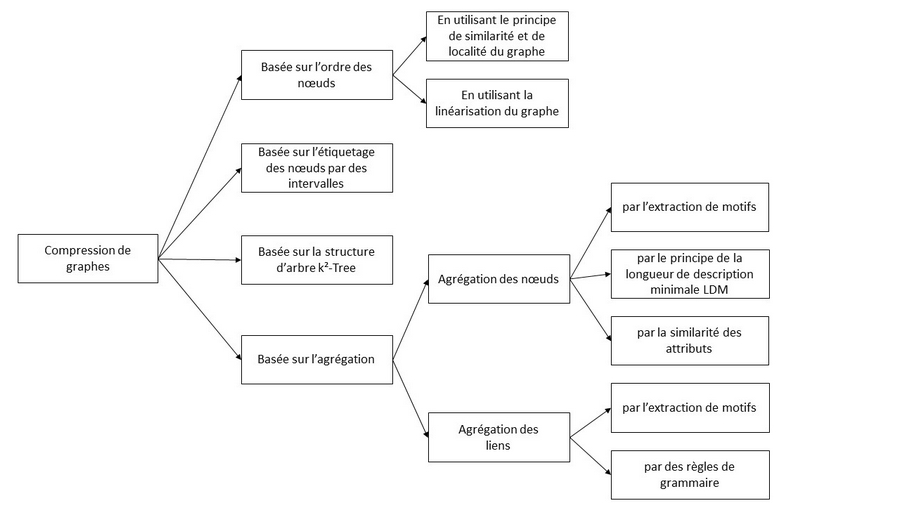
\includegraphics[scale=0.65]{./ressources/image/xx.jpg}
		\caption{Classification des méthodes de compression \citep{master2017}}
		\label{xx}
	\end{figure}


%Après l'étude des méthodes basées sur l'agrégation par extraction de motifs, nous avons constaté que certaines classes ne sont pas bien définies. Les imperfections que nous avons remarqué peuvent être énumérées comme suit : 1) les méthodes d'extraction de motifs englobent certaines méthodes d'agrégation et non pas le contraire, 2) Les méthodes d'extraction de motifs ne sont pas toutes des méthodes agrégatives, nous trouvons parmi elles d'autres méthodes basées sur un vocabulaire. Nous avons donc apporté des modifications sur cette classification. La figure \ref{classif} représente la classification de l'année passé après raffinement où nous avons marqué nos apports en rouge.

Après l'étude des méthodes basées sur l'agrégation par extraction de motifs, nous avons constaté que certaines classes ne sont pas bien définies. Nous avons remarqué que la classification a proposé d'inclure les méthodes basées sur l'extraction de motifs dans deux classes de méthodes qui sont : les méthodes basée sur l'agrégation des liens et les méthodes  basée sur l'agrégation des nœuds, or ce sont les méthodes d'extraction de motifs qui englobent certaines méthodes d'agrégation et non pas le contraire. En effet, notre étude bibliographique a clairement montré que les méthodes de compression de graphe par extraction de motifs ne sont pas toutes des méthodes agrégatives. Nous trouvons, par exemple, certaines de ces méthodes qui donnent en sortie une liste des motifs les plus pertinents du graphe avec une matrice d'erreurs sans avoir recours à l'agrégation. Donc nous avons proposé de dissocier la classe des méthodes basées sur l'extraction de motifs de la classe des méthodes basées sur l'agrégation.
En outre, nous avons considéré, contrairement à la classification précédente, que les méthodes de compression basées sur les règles de grammaire font parties des méthodes de compression par extraction de motifs. Nous justifiant cela par le fait que ces méthodes utilisent l'un des deux principes suivants : 
\begin{enumerate}
\item La transformation de la liste d'adjacence en une chaine de caractères et le remplacement, de manière itérative, de la sous-chaine de longueur deux la plus fréquente par une règle de production.
\item La recherche d'un motif, de type \textit{digram}\footnote{Un digramme : est sous-graphe composé de deux arêtes ayant un sommet en commun.}, satisfaisant une certaine condition et le remplacement de toutes ses occurrences par une production dans la grammaire. 
\end{enumerate}
Le fait que les motifs dans le cas de cette classe n'ont pas une structure de sous-graphes connus (clique, étoile, ...) n'empêche pas que le processus appliqué est toujours le même. Nous avons essayer donc de rectifier ces imperfections tout en raffinant davantage les deux classes qui font l'objet de notre Master. 

La classe des méthodes de compression par les arbres k2-trees ne peut être encore raffinée car elles partagent toutes le même principe et diffèrent dans le type de graphe en entrée ou dans le codage en sortie.

Pour la classe des méthodes de compression par extraction de motifs, nous distinguons cinq classes: 1)les méthodes de compression basées vocabulaire faisant appel aux méthodes de clustering, 2) les méthodes de compression basées vocabulaire exploitant les propriétés de la matrice d'adjacence, 3) les méthodes de compression basées agrégation des nœuds des motifs, 4) les méthodes de compression basées agrégation des liens des motifs utilisant des règles de grammaire, 5) les méthodes de compression basées agrégation des liens des motifs faisant appel à des heuristiques de partitionnement de graphes. La première et la deuxième classe se caractérisent par l'ensemble des motifs qui est prédéfini au départ. Cependant, elles se distinguent l'une de l'autre dans le principe de fonctionnement : l'une utilise des méthodes de clustering et de détection de communautés tant dis que l'autre utilise directement la matrice d'adjacence en exploitant ses propriétés. Les trois (03) dernières classes forment l'ensemble des méthodes d'extraction de motifs basées sur l'agrégation de ces derniers. 




 La figure \ref{classif} représente la classification de l'an dernier après raffinement où nous avons mis en évidence nos apports et nos modifications en pointillé.


 \begin{figure}[H]
		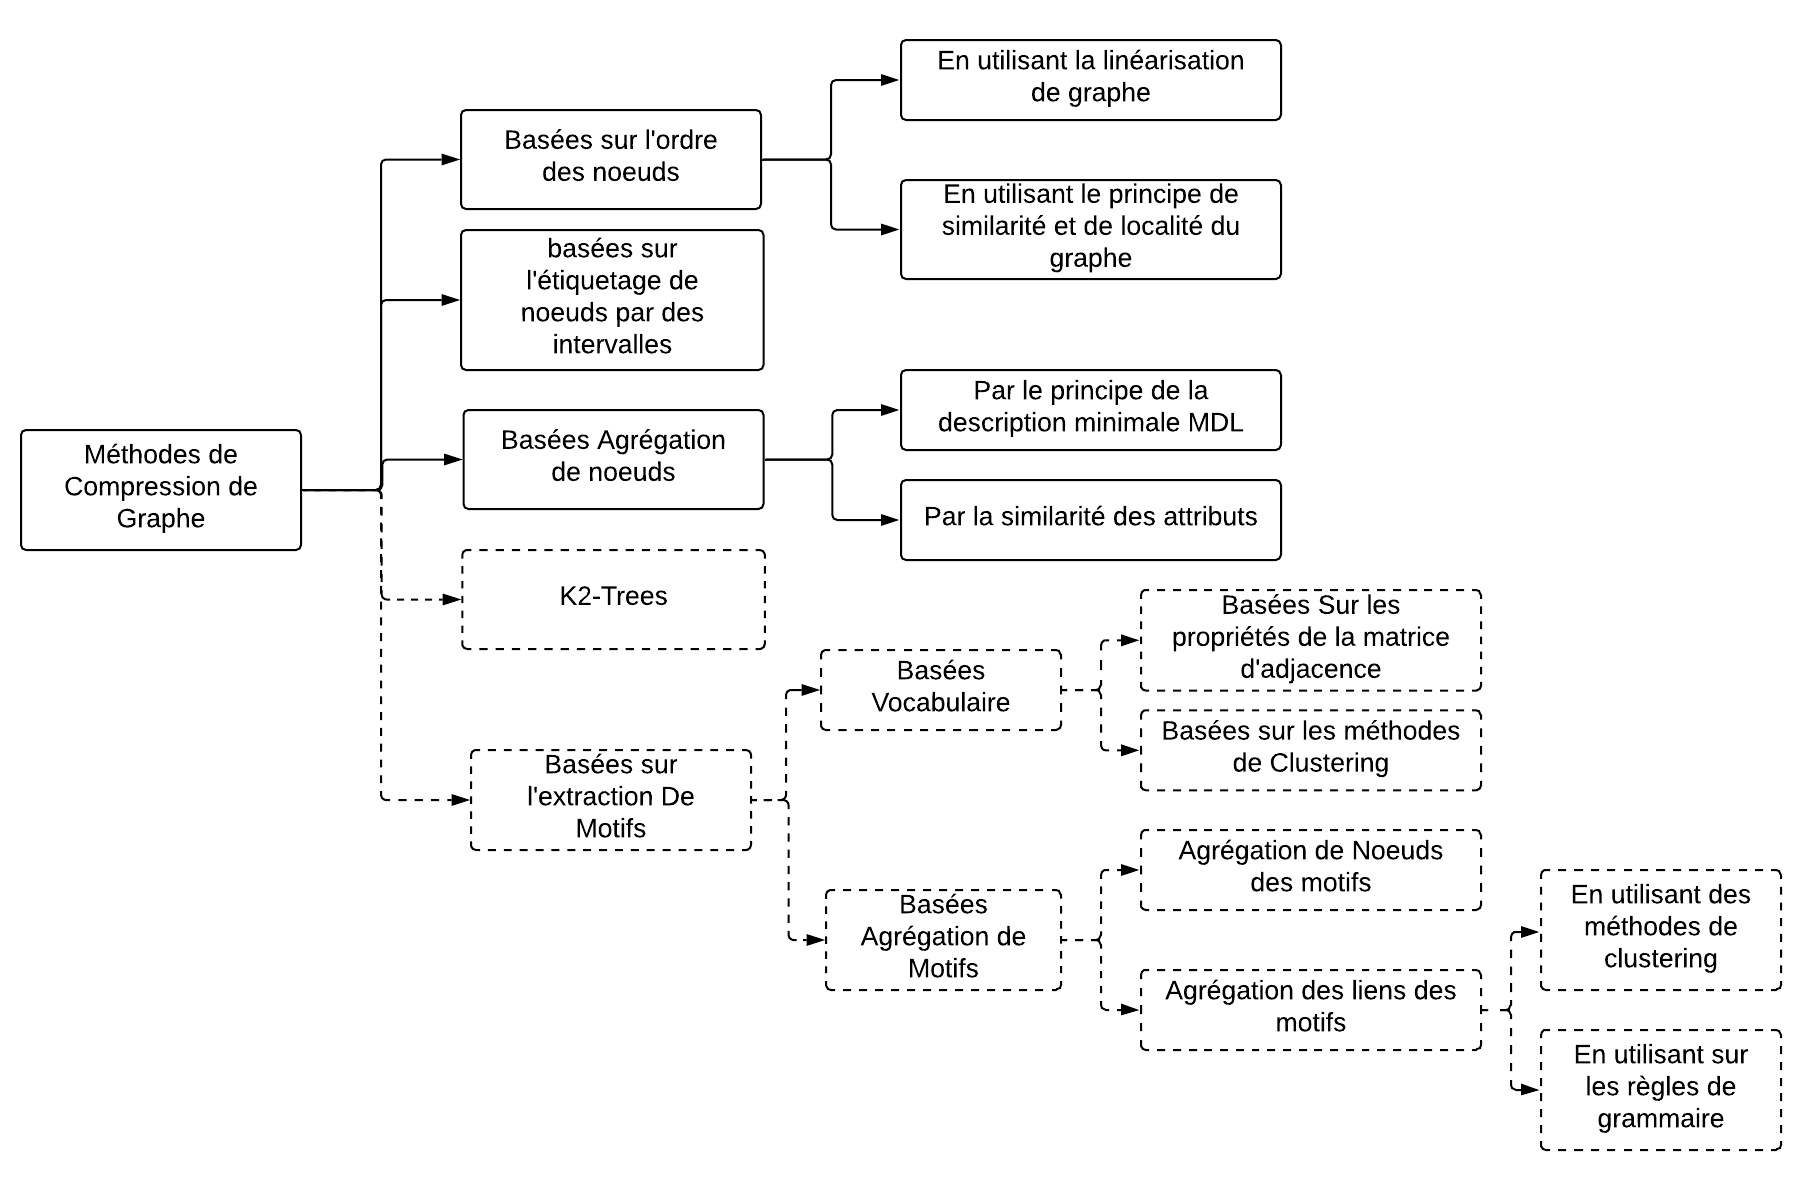
\includegraphics[scale=0.55]{./ressources/image/Classification.png}
		\caption{Classification proposées des méthodes de compression}
		\label{classif}
	\end{figure}






				
			\section{Compression par les arbres $K^2$-Trees}
				$k^2$-tree est une structure de données conçue à l'origine pour la compression des graphes du web. L'algorithme de base a été proposé par Bisaboa et al. dans leur article \textit{$k^2$-trees for Compact Web Graph} \citep{brisaboa2009k}. Elle a été appliquée ensuite dans d'autres types de données tel que les réseaux sociaux \citep{shi2012optimizing}, les données rasters \citep{de2013compact} et les bases de données \gls{rdf} \citep{alvarez2017succinct}.\\

En général, l'algorithme peut être appliqué à n'importe quelle matrice binaire. Dans le cadre de notre étude nous nous intéressons seulement à la matrice d'adjacence d'un graphe.
La compression par les $k^2$-trees exploite les propriétés de la matrice d'adjacence et tire parti des zones vides pour réduire l'espace de stockage et permettre au graphe de tenir en mémoire centrale. Il offre aussi la possibilité de naviguer dans le graphe sans le décompresser, et de répondre aux requêtes de voisinage direct et inverse.

Étant donné une matrice d'adjacence A d'ordre $|n|$, $k^2$-tree la représente sous forme d'un arbre de recherche $k^2$-aires \footnote{Les arbres n-aires sont une généralisation des arbres binaires : chaque nœud a au plus n fils.} de hauteur h = [$log_{k}$ n]. Chaque nœud de l'arbre contient un seul bit avec deux valeurs possibles : 1 pour les nœuds internes et 0 pour les feuilles, sauf le dernier niveau où les feuilles représentent les cases de la matrice A et peuvent prendre une valeur 0 ou 1. Chaque nœud interne de l'arbre a exactement $k^2$ fils.  
Avant la construction de l'arbre, il faut s'assurer que n est une puissance de k. Dans le cas contraire, l'algorithme étend la matrice en rajoutant des zéros à droite et en bas de la matrice. L'ordre de la matrice devient donc $n'= k^{log_{k} n}$.\\

Pour construire l'arbre, $k^2$-tree commence par diviser la matrice en $k^{2}$ sous matrices d'ordre $|n/k|$. La racine correspond à la matrice complète. Chaque sous matrice représente un nœud dans le premier niveau de l'arbre, elle est ajoutée comme un fils à la racine suivant un ordre de gauche à droite et de haut en bas. Le nœud est à 1 si la sous matrice qu'il représente contient au moins un 1, et à 0 si elle ne contient que des 0. Le processus est répété de manière récursive sur les sous matrices représentées par des 1. $k^{2}$ sous matrices sont considérées à chaque subdivision. L'opération est répétée jusqu'à ce que la subdivision atteint les cases de la matrice qui représenterons les feuilles de l'arbre au dernier niveau. 

La figure \ref{k2-trees-exemples} illustre la représentation $k^2$-tree d'une matrice de taille $10 \times 10$, étendue à une  taille $16 \times 16$ pour un k=2 \citep{brisaboa2015efficient}.

\begin{figure}[H]
\begin{center}
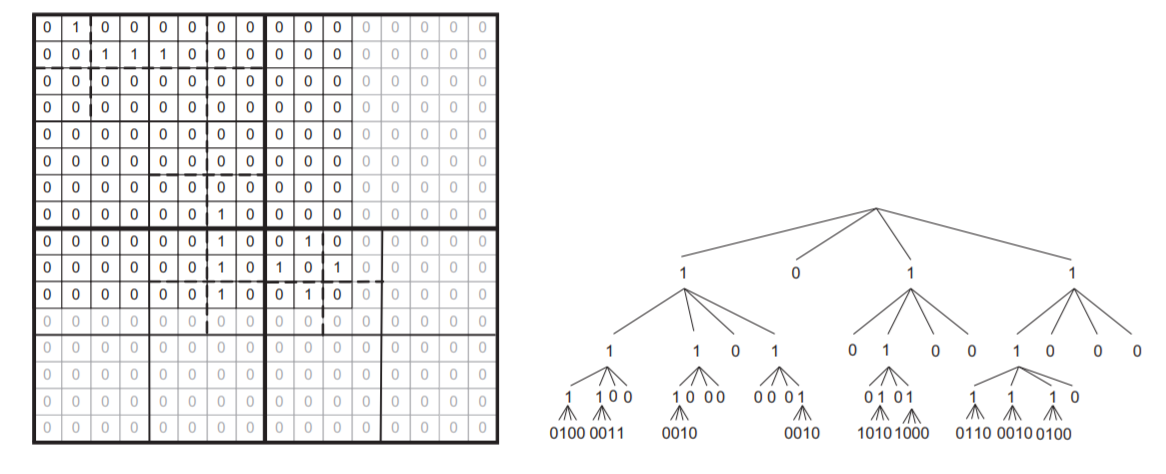
\includegraphics[height=200 pt, width=450 pt]{./ressources/image/k2-trees.png} 
\end{center}
\caption{Exemple de représentation $k^2$-tree}
\label{k2-trees-exemples}
\end{figure}


Pour le stockage de l'arbre, l'algorithme utilise deux tableaux binaires : un tableau T (Tree) contenant tous les nœuds de l'arbre à l'exception du dernier niveau et un tableau L (Leaves) contenant les feuilles du dernier niveau. Les nœuds et les feuilles sont ordonnés selon un parcours en largeur de l'arbre.   
Ci-dessous les deux tableaux T et L de l'exemple précédent (figure \ref{k2-trees-exemples}) : \\
\begin{center}
	T = 1011 1101 0100 1000 1100 1000 0001 0101 1110\\
	L = 0100 0011 0010 0010 1010 1000 0110 0010 0100\\	
\end{center}
Dans le pire des cas, l'espace total pour la description de la structure est $k^2*m(log_{k^2}\frac{n^2}{m}+ \textit{O}(1))$, où n est le nombre de nœuds du graphe et m le nombre de liens. Cependant, pour les graphes réels, l'espace nécessaire pour le stockage est bien meilleur. \\

Dans le même article \citep{brisaboa2009k}, et dans le but d'obtenir un compromis entre la taille de l'arbre et le temps de parcours, les auteurs proposent une hybridation qui consiste à changer la valeur du paramètre k en fonction du niveau de l'arbre en donnant à k une grande valeur au début pour réduire le nombre de niveaux et améliorer ainsi le temps de recherche, et une petite valeur à la fin pour avoir des petites sous matrices et réduire l'espace de stockage.
Pour le stockage de l'arbre, un tableau $T_{i}$ est utilisé pour chaque valeur $k_{i}$, le tableau L reste le même.\\

Plusieurs variantes de l'algorithme de base ont été proposées dans la littérature dont le but était soit d'obtenir un meilleur résultat de compression, soit d'appliquer la méthode sur d'autres types de graphes. Nous allons dans ce qui suit présenter les principaux travaux qui traitent ce sujet.\\

Dans \citep{shi2012optimizing}, les auteurs proposent deux techniques d'optimisation de l'algorithme : la première consiste à trouver un certain ordre des nœuds qui permet de regrouper les 1 de la matrice d'adjacence dans une seule sous matrice au lieu qu'ils soient dispersés de manière aléatoire. La recherche d'un ordre optimal des nœuds n'est pas envisageable. Avec k=2,le problème peut être réduit à un autre problème (min bisection\footnote{Le problème de bissection minimale (MBP) est un problème NP-hard bien connu, qui est destiné à diviser les sommets d'un graphe en deux moitiés égales afin de minimiser le nombre de ces arêtes avec exactement une extrémité dans chaque moitié.}) qui est NP-difficile. Les auteurs utilisent alors un parcourt \newacronym{dfs}{DFS}{Deapth First Search}\gls{dfs}
\footnote{\gls{dfs} : Parcours en profondeurs du graphe}
 avec des heuristiques pour trouver une approximation de l'ordre optimal. Cette optimisation permet de réduire le nombre de nœuds internes de l'arbre et produit ainsi un arbre optimal. La deuxième optimisation est de trouver la valeur de k la plus adéquate pour chaque nœud interne, calculer cette valeur pour chaque nœud peut engendrer un temps de calcul très important. Pour éviter cela, les auteurs affectent la même valeur k pour les nœuds ayant le même parent. 	

Dans un travail ultérieur \citep{brisaboa2014compact}, les auteurs de l'article de base apportent deux améliorations principales de leur méthode dans le but d'optimiser l'espace et le temps de parcours de l'arbre produit. La première est de construire $k^2$ arbres distincts pour les $k_{0}^{2}$ sous matrices du premier niveau. Elle présente plusieurs avantages : (1) l'espace est réduit étant donné que la taille de chaque arbre est en fonction de $\frac{n^2}{k^2}$, (2) le temps de parcours s'améliore puisque T et L sont plus petits. La deuxième amélioration est la compression de L qui consiste à construire un vocabulaire \textit{V} de toutes les sous matrices du dernier niveau sous forme de séquences de bits, les classer par fréquence d'apparition et remplacer leurs occurrences dans L par des pointeurs. Cela permet d'éviter la redondance et de réduire la taille de la structure. Les pointeurs sont représentés par des codes de longueur variable ordonnés, le plus petit correspond à la sous matrice la plus fréquente. Néanmoins, cette représentation ne permet pas un accès direct dans L étant donné qu'une décompression séquentielle est nécessaire pour récupérer une position. Pour remédier à ce problème, les auteurs utilisent le principe de
\newacronym{dac}{DAC}{Directly Addressable Codes}
 \gls{dac}\footnote{\gls{dac} est une technique qui encode une séquence d'entiers ou mots en utilisant une structure à longueur variable, son avantage principale est l'accès direct au mot sans passer par le décodage.} \citep{brisaboa2013dacs} pour garantir un accès rapide au pointeur et conserver ainsi une navigation efficace.\\
Exemple : Pour la figure \ref{k2-trees-exemples}, le vocabulaire et L sont représentés comme suit :\\
\begin{center}
\textit{V}= [0010 0100 0011 1010 1000 0110]\\
L = $c_{1}c_{2}c_{0}c_{0}c_{3}c_{4}c_{5}c_{0}c_{1}$ \\
\end{center}

%\subsubsection{d$k^2$-trees}
Dans \citep{brisaboa2012compressed}, les même auteurs développent la représentation $k^2$-trees pour les graphes dynamiques. Ils proposent une nouvelle structure nommée d$k^2$-trees pour \textit{Dynamique $k^2$-trees} qui offre les même capacités de compression et fonctionnalités de navigation que le cas statique et qui permet également d'avoir des mises à jour sur le graphe. Pour atteindre ces objectifs, d$k^2$-tree remplace la structure statique de $k^2$-tree par une implémentation dynamique. Dans cette nouvelle implémentation, les deux tableaux T et L sont remplacés par deux arbres, nommés $T_{tree}$ et $L_{tree}$ respectivement. Les feuilles de $T_{tree}$ et $L_{tree}$ stockent des parties des bitmaps T et L. La taille de ces feuilles est une valeur paramétrable. Les nœuds internes des deux arbres permettent d'accéder aux feuilles et de les modifier.
Chaque nœud interne de $T_{tree}$ contient trois(03) éléments : deux compteurs b et o, qui contiennent respectivement le nombre de bits et le nombre de "1" stockés dans les feuilles descendantes de ce nœud, et un pointeur P vers le nœud fils. Les nœuds internes de $L_{trees}$ sont similaires sauf qu'ils ne contiennent que b et P. Avec cette structuration, $T_{tree}$ et $L_{tree}$ permettent la mise à jour directe de l'arbre $k_2-tree$ dans le cas l'ajout et la suppression des liens dans le graphe.\\
La figure \ref{dk2-trees} présente une représentation d$k^2$-tree \citep{brisaboa2012compressed}: 
\begin{figure}[H]
\begin{center}
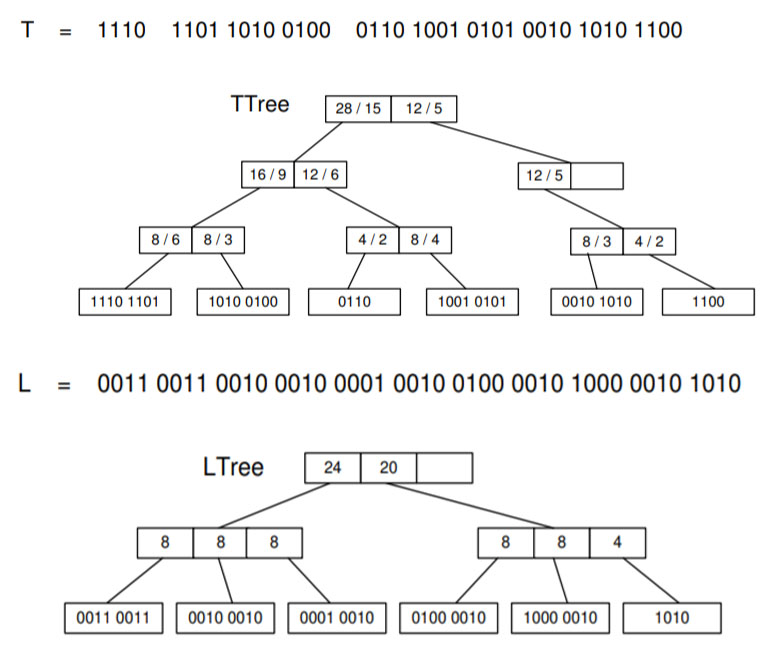
\includegraphics[scale=0.7]{./ressources/image/dk2-trees.jpg} 
\end{center}
\caption{Exemple d'une représentation d$k^2$-tree}
\label{dk2-trees}
\end{figure}

%\subsubsection{$k^n$-trees}
 Sandra et al. \citep{de2013compact} présentent $k^n$-tree, une généralisation des $k^2$-tree pour les problèmes multidimensionnels. Cette méthode possède plusieurs applications. Elle est utilisée pour représenter les bases de données multidimensionnelles, les données rasters et les graphes dynamiques. $k^n$-tree repose sur $k^2$-tree pour représenter une matrice à n-dimensions (dites \textit{tensor} en Anglais). La matrice est décomposé en $k^n$ sous-matrices de même taille, comme suit : sur chaque dimension, K-1 hyperplans devisent la matrice dans les positions i*$\frac{n}{K}$,pour $i \in [1, K-1]$. Une fois les dimensions partitionnées, $k^n$ sous-matrices sont induites, elles sont représentées par des nœuds dans l'arbre comme dans l'algorithme de base. Les structures utilisées pour le stockage sont aussi les mêmes (T et L).
En posant n=3, la méthode peut être appliquée sur les graphes dynamiques ou temporels. Ce type de graphe est représenté par une grille à 3 dimensions $X \times Y \times T$, où les deux premières dimensions représentent les nœuds de départ et de destination, et la troisième dimension représente le temps. 
La figure \ref{kn-trees} présente une représentation $k^3$-tree d'un graphe dynamique \citep{de2014new}.

\begin{figure}[H]
\begin{center}
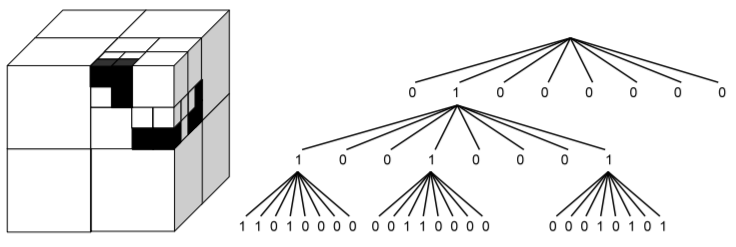
\includegraphics[height=100 pt, width=380 pt]{./ressources/image/kn-trees.png} 
\end{center}
\caption{Exemple d'une représentation $k^3$-tree}
\label{kn-trees}
\end{figure}



%\subsubsection{$K^2$-tress1 }
La représentation de base des arbres k2-trees regroupe seulement les zones de zéros, puisqu'elle a été conçue au début pour les graphes du web qui possèdent une matrice d'adjacence extrêmement creuse. Dans \citep{de2014new}, Les auteurs proposent d'étendre cette représentation en regroupant les zones de "1" également. L'idée générale est d'arrêter la décomposition de la matrice d'adjacence quand une zone unie est trouvée, à savoir des zéros ou des uns. Pour distinguer entre les différents nœuds, une représentation quadtree est utilisée \citep{de1997computational}. Une couleur est attribuée à chaque nœud, blanc pour une zone de zéro, noir pour une zone de uns et gris pour les nœuds internes, i.e, les zones contenant des uns et des zéros. Pour le stockage des nœuds, les auteurs proposent quatre encodages présentés dans ce qui suit : 

\begin{enumerate}[label=$\bullet$]
\item \textbf{ $k^2$-$trees1^{2-bits-naive}$ :} Dans cet encodage, deux bits sont utilisés pour représenter chaque type de nœud. L'attribution des bits n'est pas arbitraire, le premier bit du poids fort indique si le nœud est un nœud interne (0) ou une feuille (1), le deuxième détermine si les feuilles sont blanches (0) ou noires (1). Nous aurons donc : "10" pour les nœuds gris, "01" pour les nœuds noirs et "00" pour les nœuds blancs. Notant que les feuilles du dernier niveau sont représentées par un seul bit.
Après le codage, le premier bit de chaque nœud sauf ceux du dernier niveau est stocké dans T, un autre tableau $T'$ est créé pour sauvegarder le deuxième bit. Les nœuds du dernier niveau sont stockés dans L.
\item \textbf{ $k^2$-$tree1^{2-bits}$ :} Le même principe que l'encodage précédant sauf que les nœuds gris sont représentés par un seul bit, toujours à "1". Le tableau $T'$ va contenir dans ce cas la couleur des feuilles ce qui va réduire la taille de la structure.

\item \textbf{ $k^2$-$tree1^{DF}$ :} Cet encodage est similaire à $k^2$-$trees1^{2-bits}$, mais il utilise un seul bit pour les nœuds blancs et deux bits pour les nœuds noirs et gris, compte tenue de la fréquence des nœuds blancs dans les graphes du monde réel par rapport aux autres. Nous aurons donc : "0" pour les nœuds blancs, "10" pour les nœuds gris et "11" pour les nœuds noirs.

\item \textbf{ $k^2$-$tree1^{5-bits}$ :} Le dernier encodage repose sur la représentation de base. Un nœud blanc est représenté par "0", un nœud noir ou gris par "1", exactement comme le $k^2$-tree d'origine. Pour identifier un nœud noir (zone de uns), il sera représenté par une combinaison impossible : $k^2$ fils de "0" sont ajoutés aux nœuds noirs pour les distinguer.
\end{enumerate}


La figure \ref{k2-trees1-exemple} illustre une représentation $k^2$-tress1 avec les quatre encodages \citep{de2014new} : 


\begin{figure}[H]
\begin{center}
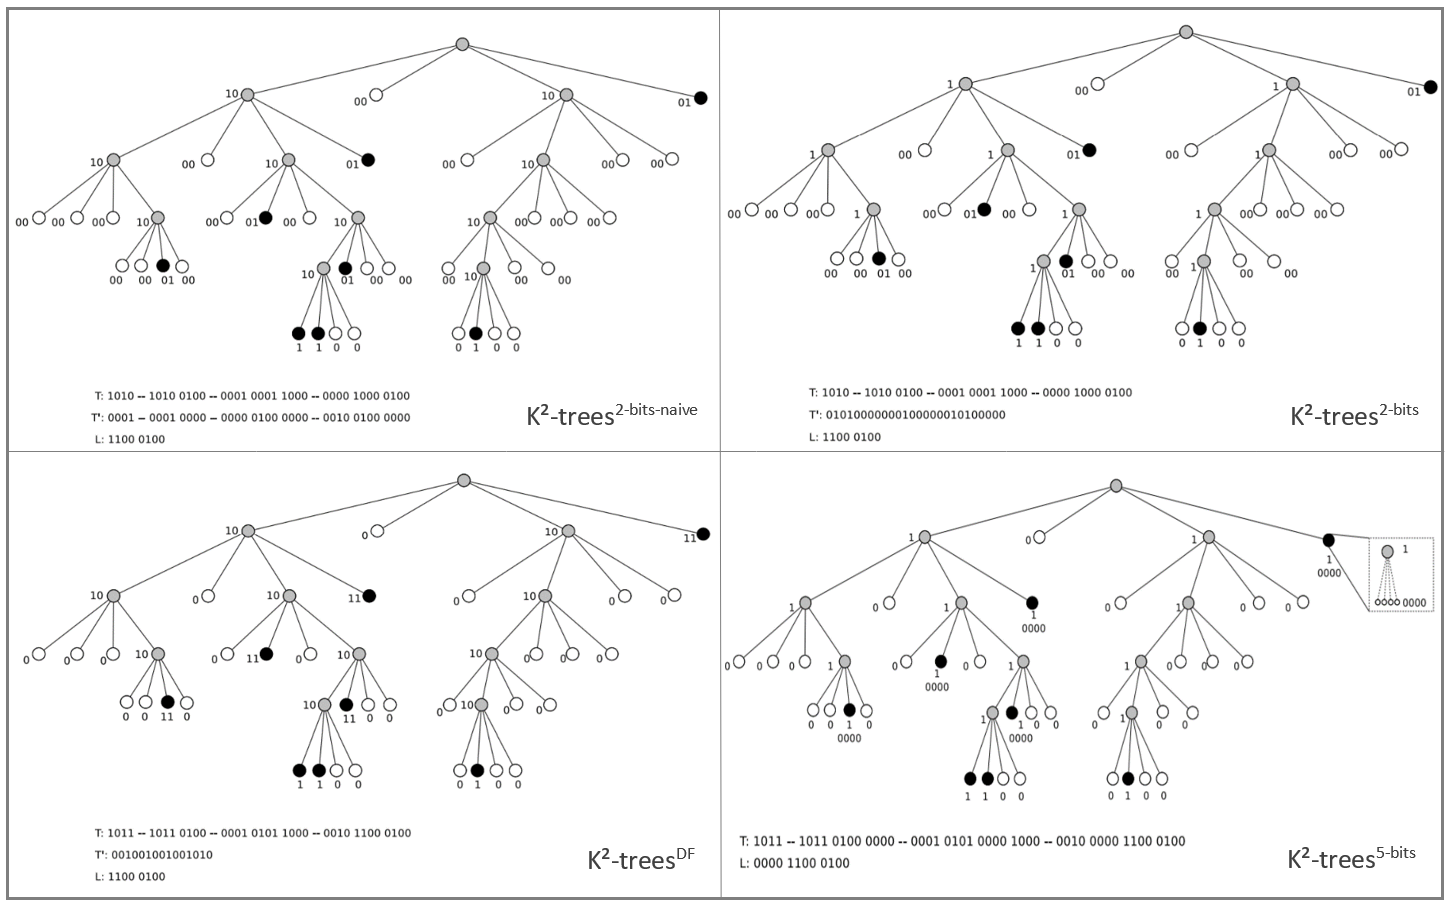
\includegraphics[height=300 pt, width=450 pt]{./ressources/image/k2-trees1.png} 
\end{center}
\caption{Exemple d'une représentation $k^2$-tree1 avec les quatre encodages}
\label{k2-trees1-exemple}
\end{figure}


%\subsubsection{Delta-$K^2$-tress }

Dans \citep{zhang2014delta}, les auteurs proposent Delta-$k^2$-tree, une variante qui exploite la propriété de similarité entre les nœuds voisins du graphe pour réduire le nombre de uns dans la matrice d'adjacence. Notons par \textit{Matrix} la matrice d'adjacence, Delta-$k^2$-trees construit une nouvelle matrice appelée \textit{Delta-matrix}, une ligne \textit{i} de \textit{Delta-matrix} va contenir la différence entre les deux lignes \textit{Matrix}[i] et  \textit{Matrix}[i-1] si cela décroit le nombre de uns sinon elle sera égale à \textit{Matrix}[i], comme suit: \\

$\left\{
\begin{array}{llcl}
\textbf{Si}\ \ count1s(matrix[i]) < countDif(matrice[i],matrix[i-1])\\
\ \ \ \ Delta-matrix[i]  := matrix[i]  \\
\textbf{Sinon} & & &\\
\ \ \ \ Delta-matrix[i]  := matrix[i] \bigoplus matrix[i-1] & 
\end{array}
\right.$\\

Où \textit{count1s} compte le nombre de 1 dans une ligne, \textit{countDif} compte le nombre de bits différents entre deux lignes et $\bigoplus$ représente le "ou exclusif".

Pour déterminer si une ligne est identique à celle de la matrice d'adjacence ou non, un tableau D est utilisé : Si D[i]=1 la ligne est identique, sinon c'est une ligne de différence.\\
La matrice \textit{Delta-matrix} contient moins de uns que la matrice d'adjacence, d'où elle est plus creuse, ce qui permet de réduire la taille de la structure et avoir un meilleur taux de compression. Cependant le temps de parcours est plus grand car pour accéder à certaines lignes (lignes de différence), le graphe doit être décompressé et la matrice d'adjacence reconstituée.\\
La figure \ref{k2-trees-delta} présente un exemple de la représentation Delta-$k^2$-tree \citep{zhang2014delta}.


\begin{figure}[H]
\begin{center}
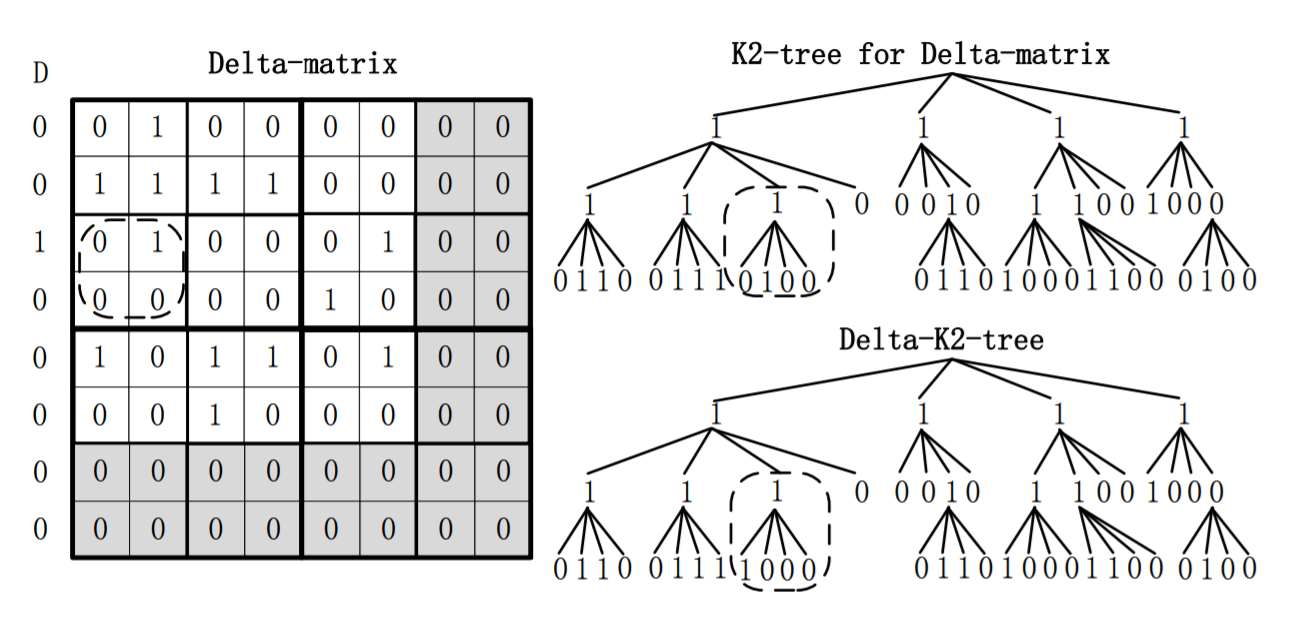
\includegraphics[height=150 pt, width=380 pt]{./ressources/image/k2-trees-delta.png} 
\end{center}
\caption{Exemple d'une représentation Delta-$k^2$-tree}
\label{k2-trees-delta}
\end{figure}

%\subsubsection{$K^2$-treaps }
$K^2$-treap est une autre variante de $k^2$-tree, elle a été proposée dans \citep{brisaboa2014k}. Cette variante combine les $k^2$-trees avec une autre structure de données appelée treap \footnote{Les Treaps sont des arbres de recherche binaire avec des nœuds ayant deux attributs : clé et priorité. La recherche dans ces arbres s'effectue selon ces attributs.} \citep{aragon1989randomized}. Les auteurs appliquent cette méthode sur des grilles multidimensionnelles comme 
\newacronym{olap}{OLAP}{Online Analytical Processing}
\gls{olap} pour pouvoir les stocker et répondre efficacement aux requêtes top-K \citep{badr2013traitement}. La méthode peut être également appliquée sur les graphes pondérés, où chaque case de la matrice d'adjacence du graphe comporte le poids de l'arête qu'elle représente au lieu d'un 1.
Comme dans l'algorithme de base, une décomposition récursive en $k^2$ sous-matrices est appliquée sur la matrice d'adjacence et un arbre $k^2$-air est construit comme suit : la racine de l'arbre va contenir les coordonnées ainsi que la valeur de la cellule ayant le plus grand poids de la matrice. La cellule ajoutée à l'arbre est ensuite supprimée de la matrice. Si plusieurs cellules ont la même valeur maximale, l'une d'elles est choisie au hasard. Ce processus est répété récursivement sur chaque sous matrice. La procédure continue sur chaque branche de l'arbre jusqu'à ce qu'on tombe sur les cellules de la matrice d'origine ou sur une sous matrice complètement vide (contient que des zéros).\\
La figure \ref{k2-treaps} suivante illustre la représentation $k^2$-treap d'un graphe pondéré \citep{badr2013traitement} :

\begin{figure}[H]
\begin{center}
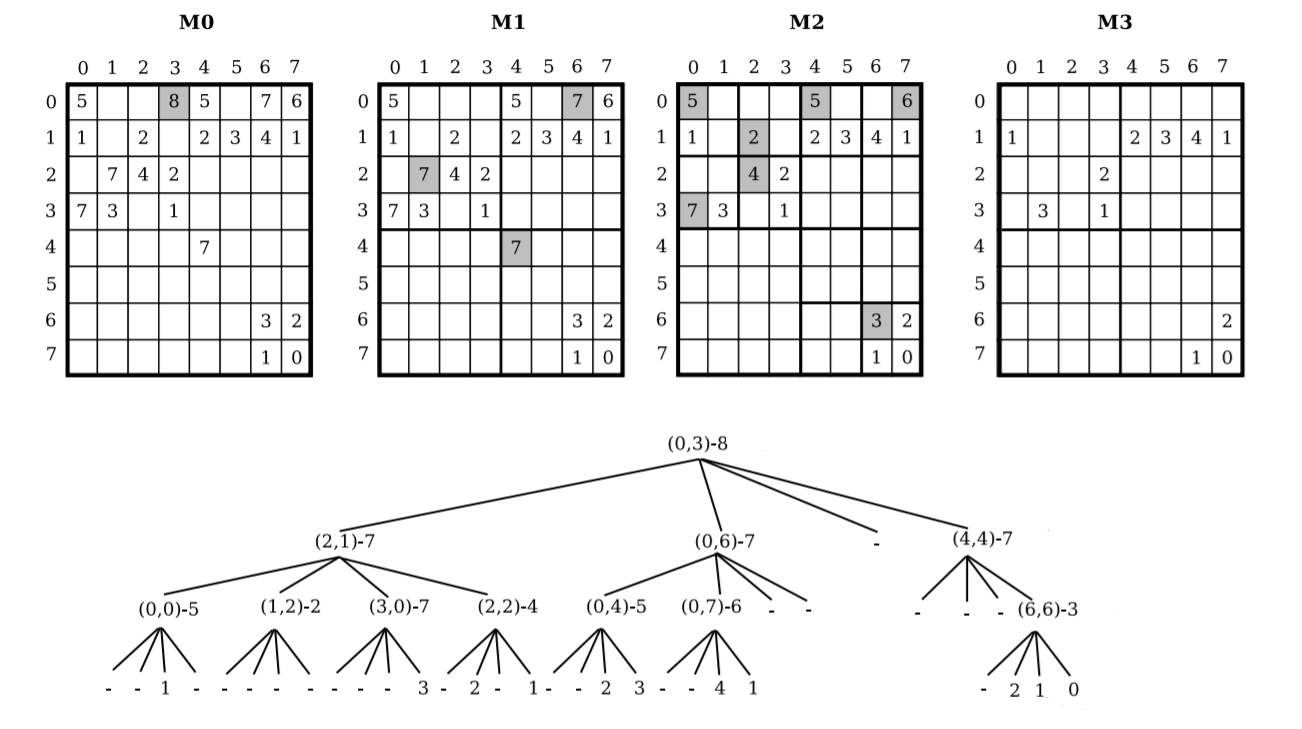
\includegraphics[height=200 pt, width=380 pt]{./ressources/image/k2-treaps.png} 
\end{center}
\caption{Exemple d'une représentation $k^2$-treap d'un graphe pondéré}
\label{k2-treaps}
\end{figure}

Pour avoir une bonne compression, $k^2$-treap effectue des transformations sur les données stockées. La première transformation consiste à changer les coordonnées représentées dans l'arbre en des coordonnées relatives par rapport à la sous matrice actuelle. La deuxième est de remplacer chaque poids dans l'arbre par la différence entre sa valeur et celle de son parent.\\
Trois structures de données sont utilisées pour sauvegarder les coordonnées et les valeurs des cellules ainsi que la topologie de l'arbre. Chaque structure est détaillée dans ce qui suit :
\begin{itemize}
\item \textit{Listes de coordonnées locales :} La séquence de coordonnées de chaque niveau \textit{l} de l'arbre est stockée dans une liste \textit{coord}[\textit{l}].
\item \textit{Liste des valeurs : } Le parcours de l'arbre se fait en largeur, la séquence des valeurs récupérées est stockée dans une liste nommée \textit{values}. Un tableau nommé \textit{first} est utilisé pour sauvegarder la position début de chaque niveau dans \textit{values}.
\item \textit{L'arbre :} La structure de l'arbre $k^2$-treap est sauvegardée avec un arbre $k^2$-tree, les nœuds contenant des valeurs dans $k^2$-treap sont représentés par des uns et les nœuds vides par des zéros. Pour le stockage de l'arbre, un seul tableau T est utilisé. 
\end{itemize}

La figure \ref{k2-treaps-structure} représente les structures de données utilisées pour le stockage de l'arbre de la figure \ref{k2-treaps} précédente \citep{badr2013traitement} :

\begin{figure}[H]
\begin{center}
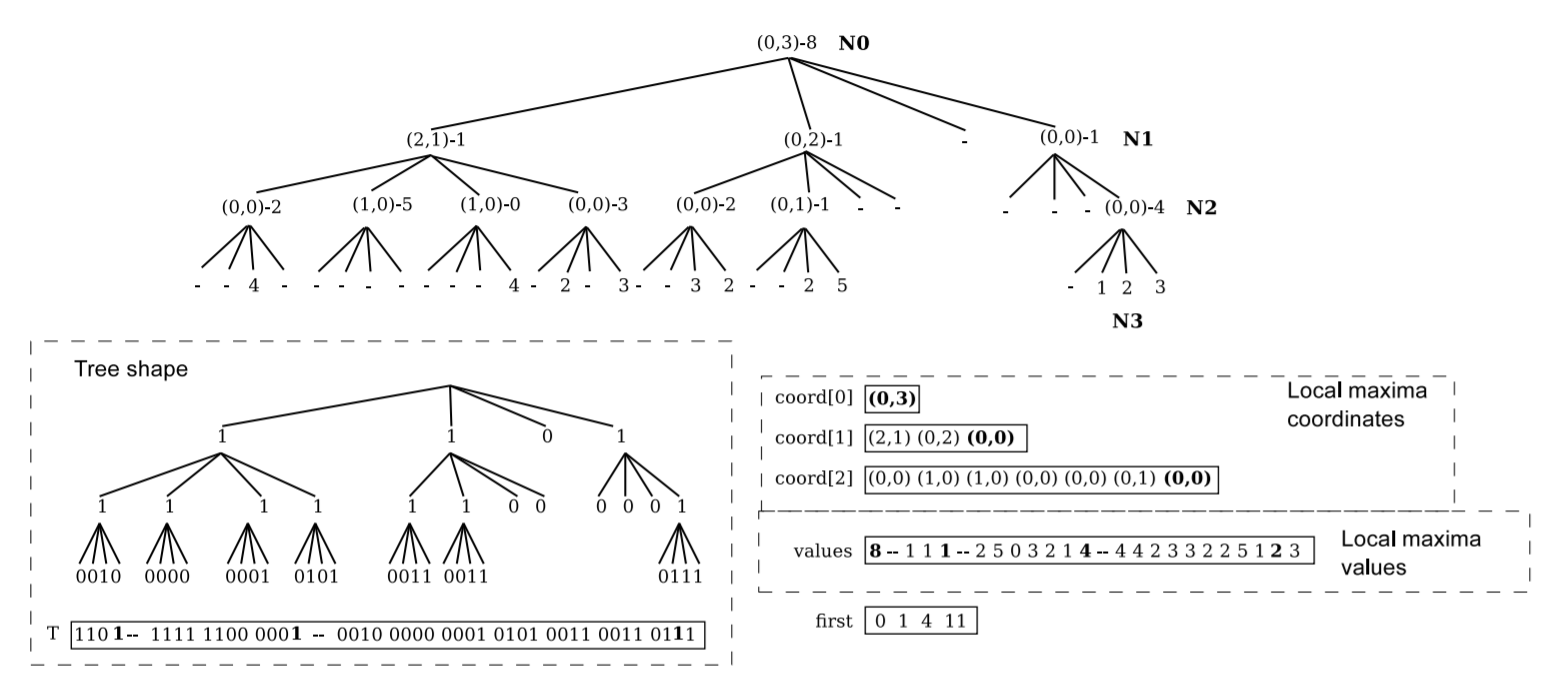
\includegraphics[height=200 pt, width=380 pt]{./ressources/image/k2-treaps-structure.png} 
\end{center}
\caption{Structures de données pour une représentation $k^2$-treap}
\label{k2-treaps-structure}
\end{figure}

%\subsubsection{I$k^2$-trees}
Garcia et al. \citep{garcia2014interleaved} proposent I$k^2$-tree pour Interleaved $k^2$-tree. Elle est appliquée sur les bases de données RDF ainsi que sur les graphes dynamiques. Dans les graphes dynamiques, les deux premières dimensions correspondent aux nœuds source et destination et la troisième dimension reflète le temps. Le graphe est donc défini par |T| matrices d'adjacence prisent à des instants $t_k$ différents. I$k^2$-tree représente les matrices simultanément. Chaque matrice est représentée par un arbre $k^2$-tree et ils sont par la suite regroupés dans un seul arbre. Chaque nœud de l'arbre obtenu représente une sous-matrice comme dans l'algorithme de base, sauf qu'au lieu d'utiliser un seul bit, I$k^2$-tree utilise 1 à |T| bits pour représenter le nœud. Le nœud racine contient |T| bits. Le nombre de bits de chaque fils dépend du nombre de uns de son parent. L'arbre finale est toujours stocké avec deux tableaux : T et L.
La figure \ref{Ik2-trees} est un exemple de I$k^2$-tree appliqué sur un graphe dynamique représenté dans trois instants \citep{garcia2014interleaved} :

\begin{figure}[H]
\begin{center}
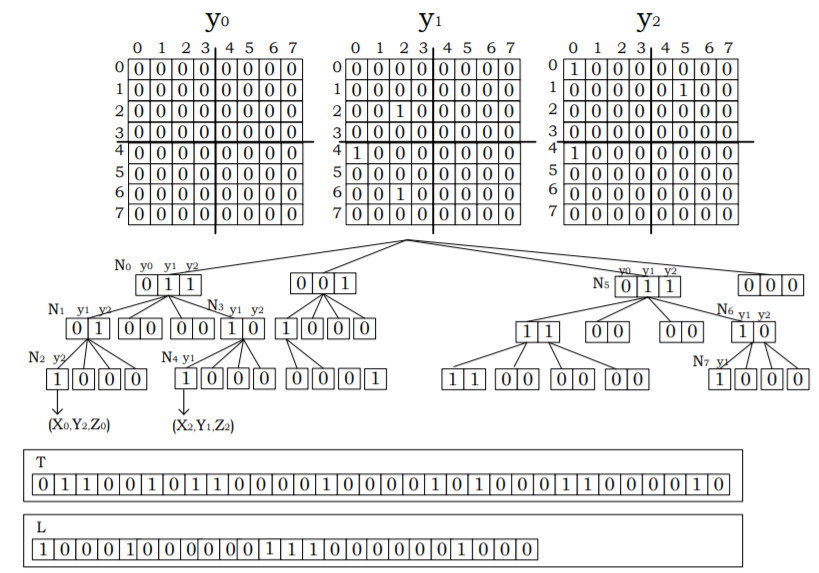
\includegraphics[scale=0.55]{./ressources/image/Ik2-trees.png} 
\end{center}
\caption{Exemple d'une représentation I$k^2$-tree}
\label{Ik2-trees}
\end{figure}

%\subsubsection{diff I$k^2$-trees}
Une variante de I$k^2$-tree appelée Differential I$k^2$-tree a été étudiée dans \citep{alvarez2017succinct}. Elle vise à améliorer le taux de compression en représentant uniquement les changements survenus sur le graphe à un instant $t_i$ au lieu d'une instance complète : à l'instant $t_0$, une capture complète du graphe (matrice d'adjacence) est stockée. À l 'instant $t_k$, pour k>0, seules les arrêtes qui changent de valeurs entre $t_{k-1}$ et $t_k$ sont stockées. Les matrices sont représentées à la fin de la même manière que I$k^2$-tree. La limite de cette représentation est que la structure doit être décompressée lors d'une requête.
La figure \ref{Ik2-trees-diff} montre un exemple d'une représentation diffI$k^2$-trees \citep{alvarez2017succinct}.

\begin{figure}[H]
\begin{center}
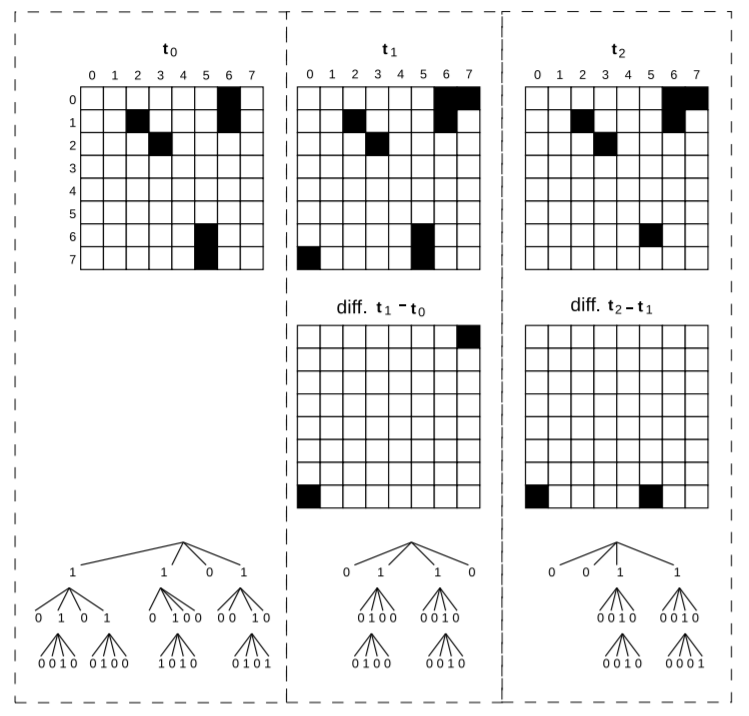
\includegraphics[scale=0.8]{./ressources/image/Ik2-trees-diff.png} 
\end{center}
\caption{Exemple d'une représentation diff I$k^2$-tree}
\label{Ik2-trees-diff}
\end{figure}

%\subsubsection{Att $K^2$-trees }
Dans \citep{alvarez2018compact}, les auteurs étendent la représentation $k^2$-tree pour les bases de données orientées graphes. Ces graphes sont étiquetés, attribués, orientés et ont des arêtes multiples. Ils présentent le graphe sous forme d'une nouvelle structure intitulée Att$k^2$-tree pour Attributed $k^2$-trees.
La figure \ref{k2-trees-att-graphe} montre un exemple de graphe pris en compte par Att$K^2$-tree \citep{alvarez2018compact}.

\begin{figure}[H]
\begin{center}
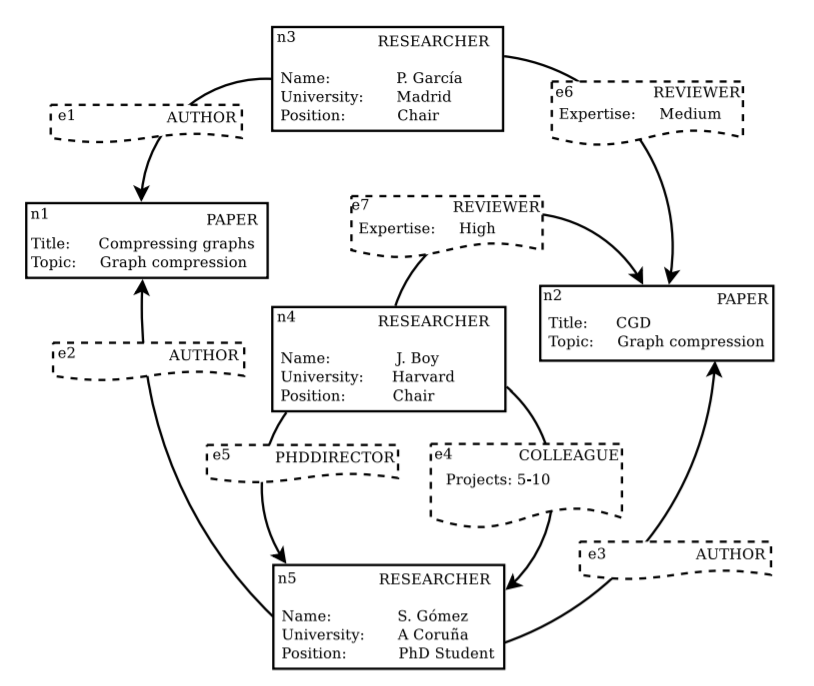
\includegraphics[height=200 pt, width=280 pt]{./ressources/image/k2-trees-att-graphe.png} 
\end{center}
\caption{Exemple d'un graphe étiqueté, attribué, orienté et multiple}
\label{k2-trees-att-graphe}
\end{figure}

\textbf{Structures de données :} La représentation obtenue par la compression est composée d'un ensemble d'arbres $k^2$-tree et d'autres structures supplémentaires. Le graphe est représenté par trois composantes: un schéma de données, les données incluses dans les nœuds et les liens et finalement la relation entre les éléments du graphe. Chaque composant est présenté dans ce qui suit :
\begin{itemize}
\item \textit{Schéma : } Ce composant gère les étiquettes et les attributs de chaque type d'éléments, il joue le rôle d'un index dans la représentation. Il est composé de :
\begin{description}
\item[Un schéma de nœuds :] représenté par un tableau qui contient les étiquettes des nœuds ordonnées lexicographiquement. Un identifiant est attribué à chaque nœud du graphe selon l'ordre du tableau, les \textit{$m_1$} nœuds possédant la première étiquette du tableau vont avoir des identifiants de 1 à \textit{$m_1$}, les \textit{$m_2$} nœuds avec la deuxième étiquette du tableau vont avoir des identifiants de \textit{$m_1$}+1 à \textit{$m_1$}+\textit{$m_2$} et ainsi de suite. Chaque entrée du tableau va ainsi stocker le plus grand identifiant portant son étiquette, cela permet de trouver l'étiquette d'un nœud à travers son identifiant.
\item[Un schéma d'arêtes :] Comme dans le cas des nœuds, un tableau est utilisé pour stocker les étiquettes des arêtes avec le même principe.  
\end{description}
Le schéma est le point de départ de la représentation, il permet d'obtenir l'étiquette d'un nœud ou d'une arête, et d'accéder à ses attributs.
\item \textit{Données :} Ce composant contient toutes les valeurs que peut prendre un attribut dans le graphe. Un attribut peut être représenté de deux façons différentes selon sa fréquence d'apparition, on distingue donc deux types d'attributs :
\begin{description}
\item[Attributs rares :] Ce sont les attributs qui prennent généralement des valeurs différentes à chaque apparition, ils sont stockés dans des listes et indexés avec l'identifiant de l'élément.
\item[Attributs fréquents :] Ce type d'attributs est sauvegardé dans deux matrices, une pour les attributs des nœuds et l'autre pour les attributs des liens. Les matrices sont stockées sous forme d'arbres $k^2$-trees.
\end{description}
La figure \ref{k2-trees-att-schema} illustre les deux composants schéma et données de la représentation Att$k^2$-trees  de la figure \ref{k2-trees-att-graphe} \citep{alvarez2018compact}:
\begin{figure}[H]
\begin{center}
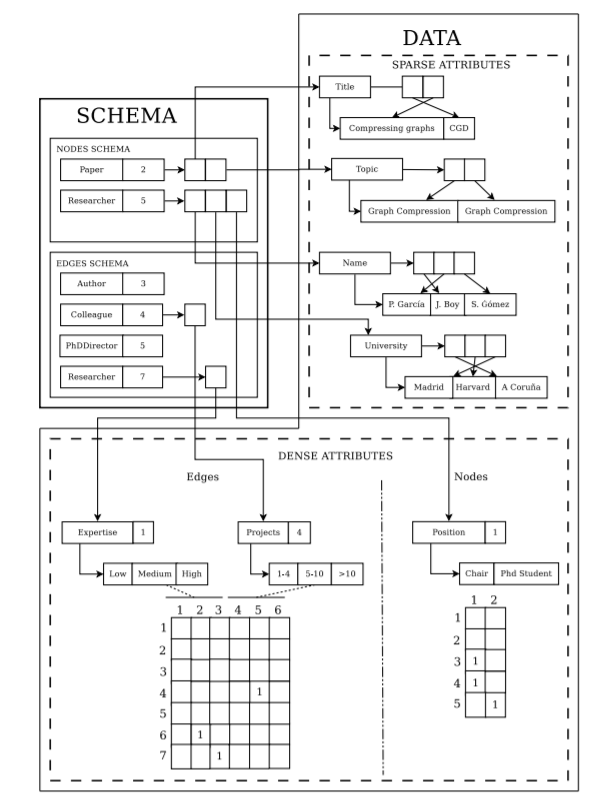
\includegraphics[scale=0.7]{./ressources/image/k2-trees-att-schema.png} 
\end{center}
\caption{Exemple d'une représentation Att$k^2$-tree (1/2)}
\label{k2-trees-att-schema}
\end{figure}


\item \textit{Relations :} C'est le dernier composant de Att$k^2$-tree, il stocke les relations entre les nœuds et les arêtes du graphe en utilisant un arbre $k^2$-tree et d'autres structures pour sauvegarder les identifiants des arêtes ainsi que les arêtes multiples. Les structures supplémentaires sont les suivantes :
\begin{description}
\item[Multi :] Un tableau qui indique si l'arête est multiple ou non.
\item[Firt :] Un tableau qui donne l'identifiant de l'arête, ou de celui de la première dans le cas d'une arrête multiple.
\item[Next :] Un tableau qui contient les identifiants des arêtes multiples restantes.
\end{description}
La figure \ref{k2-trees-att-relation} donne la représentation Att$k^2$-tree des relations du graphe de la figure \ref{k2-trees-att-graphe} \citep{alvarez2018compact}:
\begin{figure}[H]
\begin{center}
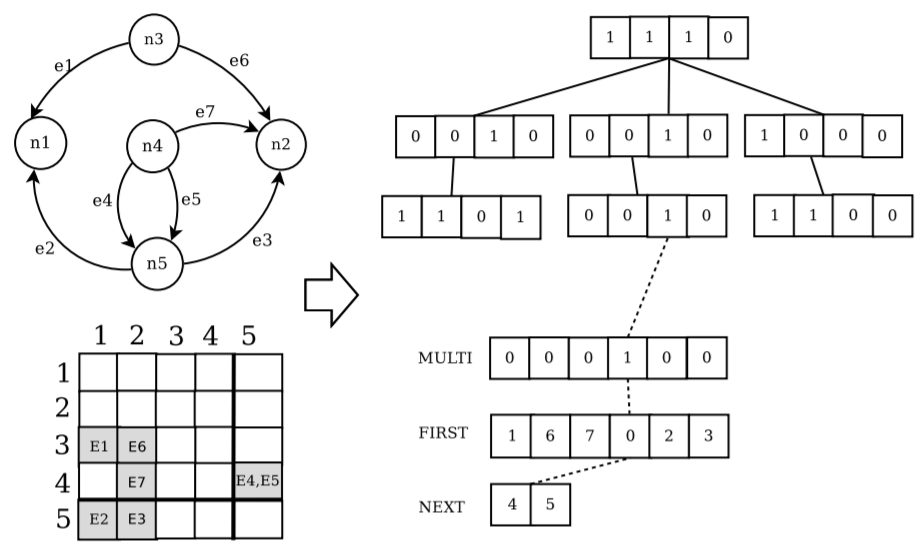
\includegraphics[height=200 pt, width=280 pt]{./ressources/image/k2-trees-att-relation.png} 
\end{center}
\caption{Exemple d'une la représentation Att$k^2$-tree (2/2)}
\label{k2-trees-att-relation}
\end{figure} 
\end{itemize}

%\subsubsection{dynAtt$k^2$-trees }
Dans le même article \citep{alvarez2018compact}, les auteurs étendent Att$k^2$-tree pour les graphes dynamiques. Ils proposent une nouvelle variante appelée dynAtt$k^2$-tree qui supporte le changement dans les attributs et les liens du graphe. Comme Att$k^2$-tree, dynAtt$k^2$-tree représente le graphe avec trois composantes : Schémas, données et relations. Les composantes sont semblables à ceux de Att$k^2$-tree mais avec certaines amélioration vue la nature dynamique du graphe.\\
\textbf{Structure de données : } 
\begin{itemize}
\item \textit{Schéma :}  En ce qui concerne les nœuds, leurs étiquettes sont stockées dans une liste dynamique ordonnée lexicographiquement. En outre, une séquence dynamique est utilisée pour sauvegarder le type de chaque nœud. Elle est stockée ensuite sous forme d'un arbre d'ondelettes \footnote{Ou wavelet en anglais, est un arbre binaire équilibré qui contient des données compressées dans une représentation optimale.} \citep{grossi2003high}. Le même principe est appliqué sur les arrêtes. 
\item \textit{Données :} Les attributs rares sont stockés dans des listes dynamiques, quant aux attributs fréquents, ils sont sauvegardés avec des arbres d$k^2$-trees (un arbre pour chaque attribut).
\item \textit{Relations :} Le stockage des relations se fait à l'aide d'un d$k^2$-tree et des tableaux dynamiques pour stocker les identifiants des arêtes et les arêtes multiples.
\end{itemize}





























																		\begin{landscape}
								\begin{table}
									\begin{tabular}{|C{6cm}|c|c|c|c|c|c|c|c|c|c|c|c|c|}
										\hline
										\multirow{2}{*}[-25pt]{     Article   }  & \multicolumn{5}{c|}{Graphe en entrée} & \multicolumn{2}{c|}{Compression} & \multicolumn{2}{c|}{Structure en sortie} & \multirow{2}{*}[-25pt]{Graphe de test} & \multirow{2}{*}[-25pt]{Résultat}  \\ \cline{2-10}
				     & \rotatebox[origin=c]{90}{ Orienté }  & \rotatebox[origin=c]{90}{ Non orienté } & \rotatebox[origin=c]{90}{ Statique } & \rotatebox[origin=c]{90}{ Dynamique } & \rotatebox[origin=c]{90}{ Autre Propriétés } &  \rotatebox[origin=c]{90}{ Avec perte } & \rotatebox[origin=c]{90}{ Sans perte } & \rotatebox[origin=c]{90}{ Succincte } & \rotatebox[origin=c]{90}{ Structurelle } & & \\ \hline				%%%%%%Fin du header
				
\hline  $k^2$-trees : Algorithme de base
   \citep{brisaboa2009k} 
   & \cmark & \cmark & \cmark & \xmark &  & \xmark &  \cmark & \cmark & \xmark	 & 		
	\begin{minipage}[t]{0.15\textwidth}
	eu-2005\\
	
	cond-mat
  \end{minipage}	
										 &
	\begin{minipage}[t]{0.2\textwidth}
	 5.21 bits/lien \\
	 16.88\% \\
	 15.58\% 
  \end{minipage}	\\

\hline $k^2$-trees : Hybridation \citep{brisaboa2009k} & \cmark & \cmark & \cmark & \xmark &  & \xmark &  \cmark & \cmark & \xmark  & 
										\begin{minipage}[t]{0.15\textwidth}
	eu-2005
  \end{minipage}	
										 &
	\begin{minipage}[t]{0.2\textwidth}
	 5.21 bits/lien 
  \end{minipage}	\\  
\hline $k^2$-trees : Optimisation \citep{shi2012optimizing} & \cmark & \cmark & \cmark & \xmark &  & \xmark &  \cmark & \cmark & \xmark  & 
\begin{minipage}[t]{0.15\textwidth}
	cond-mat
  \end{minipage}	
										 &
	\begin{minipage}[t]{0.2\textwidth}
	
	 37.96\% 
  \end{minipage}	\\
  			\hline
  			
\hline $k^2$-trees : Amélioration \citep{brisaboa2014compact} & \cmark & \cmark & \cmark & \xmark &  & \xmark &  \cmark & \cmark & \xmark  & 
  				\begin{minipage}[t]{0.15\textwidth}
	eu-2005
  \end{minipage}	
										 &
	\begin{minipage}[t]{0.2\textwidth}
	
	 3.22 bits/lien
  \end{minipage}	\\
  				
  				\hline  		
  			
\hline d$k^2$-trees \citep{brisaboa2012compressed} & \cmark & \cmark & \xmark & \cmark &  & \xmark &  \cmark & \cmark & \xmark  &
  				\begin{minipage}[t]{0.15\textwidth}
	eu-2005
  \end{minipage}	
										 &
	\begin{minipage}[t]{0.2\textwidth}
	
	 6.2 bits/lien
  \end{minipage}	\\
  \hline 
  			
\hline $k^n$-trees \citep{de2013compact} & \cmark & \cmark & \xmark & \cmark & & \xmark & \cmark & \cmark & \xmark  &
  				\begin{minipage}[t]{0.15\textwidth}
	CommNet
  \end{minipage}	
										 &
	\begin{minipage}[t]{0.2\textwidth}
	
	 65.16\% 
  \end{minipage}	\\
  \hline  	

	

  			
\hline $k^2$-trees1\citep{de2014new} & \cmark & \cmark & \cmark & \xmark & & \xmark & \cmark & \cmark & \xmark  & 
  							\begin{minipage}[t]{0.1\textwidth}
	eu-2005
  \end{minipage}	
										 &
	\begin{minipage}[t]{0.2\textwidth}
	 16.23\% 
  \end{minipage}	\\
  \hline  
  			
\hline Delta-$k^2$-trees  \citep{zhang2014delta} & \cmark & \cmark & \cmark & \xmark & & \xmark & \cmark & \cmark & \xmark  & 
  							\begin{minipage}[t]{0.1\textwidth}
	eu-2005
  \end{minipage}	
										 &
	\begin{minipage}[t]{0.2\textwidth}
	 3.24 bits/lien 
  \end{minipage}	\\
  \hline  
  
\hline $k^2$-treaps  \citep{brisaboa2014k} & \cmark & \cmark & \cmark & \xmark & 
\begin{minipage}[t]{0.15\textwidth}
  			Pondéré 
  \end{minipage}		
   & \xmark & \cmark & \cmark & \xmark  & 
  							\begin{minipage}[t]{0.1\textwidth}
	SalesDay
  \end{minipage}	
										 &
	\begin{minipage}[t]{0.2\textwidth}
	 2.48 bits/lien
  \end{minipage}	\\
  \hline  
 
\hline I$k^2$-trees  \citep{garcia2014interleaved} & \cmark & \cmark & \xmark & \cmark & & \xmark & \cmark & \cmark & \xmark  & 
  							\begin{minipage}[t]{0.1\textwidth}
	CommNet
  \end{minipage}	
										 &
	\begin{minipage}[t]{0.2\textwidth}
	
	 60.43\% 
  \end{minipage}	\\
  \hline  	
  			
 
\hline Diff I$k^2$-trees  \citep{alvarez2017succinct} & \cmark & \cmark & \xmark & \cmark & & \xmark & \cmark & \cmark & \xmark  & 
  							\begin{minipage}[t]{0.1\textwidth}
	CommNet
  \end{minipage}	
										 &
	\begin{minipage}[t]{0.2\textwidth}
	
	 60.43\% 
  \end{minipage}	\\
  \hline 
				
				 
\hline Att $k^2$-trees  \citep{alvarez2018compact} & \cmark & \cmark & \cmark & \xmark & 
\begin{minipage}[t]{0.1\textwidth}
  			Étiqueté\\
  			Attribué\\
  			Multiple
  \end{minipage}	
& \xmark & \cmark & \cmark & \xmark  & 
  							\begin{minipage}[t]{0.15\textwidth}
	Movielen-10M
  \end{minipage}	
										 &
	\begin{minipage}[t]{0.2\textwidth}
	
	 89.97\% 
  \end{minipage}	\\
  \hline 
  			
\hline dynAtt $k^2$-trees  \citep{alvarez2018compact} & \cmark & \cmark & \xmark & \cmark & 
\begin{minipage}[t]{0.1\textwidth}
  			Étiqueté\\
  			Attribué\\
  			Multiple
  \end{minipage}	
& \xmark & \cmark & \cmark & \xmark  & 
			\begin{minipage}[t]{0.1\textwidth}
	Movielen-10M
  \end{minipage}	
										 &
	\begin{minipage}[t]{0.2\textwidth}
	
	93.75\% 
  \end{minipage}	\\  				
  				\hline 
				
									\end{tabular}
									\caption{Synthèse des méthodes de compression par $k^2$-trees.}									
									
								\end{table}
								
							\end{landscape}				
			\section{Compression par extraction de motifs}
			 Les motifs fréquents sont des connaissances extraites sur des données. Leur but est de fournir à l'utilisateur des informations non triviales, implicites, présumées non connues. Ils lui offrent ainsi une meilleure appréhension des données. Dès lors, l'extraction de motifs fréquents est  devenue une tâche importante dans la fouille de données et un thème très étudié par la communauté. Elle a aussi été vastement %%%% verifier ce mot
			 utilisée dans le domaine de compression des graphes vu qu'elle permet de ne garder que l'information utile et d'éliminer les redondances de manière efficace. En effet, nous trouvons plusieurs méthodes basées sur ce principe où nous pourrons clairement distinguer deux grandes classes : 
			 (i) les méthodes de compression basées vocabulaire
			 (ii) les méthodes de compression basées agrégation.
			 
				Dans cette section, nous allons expliquer le principe de base de chaque classe et nous allons subdiviser chacune en plusieurs sous-classes en se basant sur ce dernier. 
				%%% a revoir le dernier paragraphe
			 
				\subsection{Compression basée vocabulaire}
				\label{vog_desc}
				Les méthodes de compression par extraction de motifs basées vocabulaire sont des méthodes qui ont attirées l'attention des chercheurs ces dernières années car elles permettent une meilleure compréhension du graphe. Elles partent toujours d'un ensemble de structures prédéfinies qui ont été prouvées fréquentes dans les graphes réels. Deux sous classes de cette dernières peuvent être identifiées :
				 
					 \textbf{Les Méthodes basées sur des techniques de clustering}
							
							Les méthodes de cette classe s'appuient sur le fait qu'on ne peut pas comprendre facilement les graphes denses, alors que quelques structures simples sont beaucoup plus faciles à comprendre et souvent très utiles pour analyser le graphe. Elles se basent sur des algorithmes de détection de communautés. 
							La question suivante peut alors se poser: pourquoi ne pas appliquer l'un des nombreux algorithmes de détection de communautés ou de partitionnement de graphes pour compresser le graphe en termes de communautés? La réponse est que ces algorithmes ne servent pas tout à fait le même objectif que la compression. Généralement, ils détectent de nombreuses communautés sans ordre explicite, de sorte qu'une procédure de sélection des sous-graphes les plus «importants» est toujours nécessaire. En plus de cela, ces méthodes renvoient simplement les communautés découvertes, sans les caractériser (par exemple, clique, étoile) et ne permettent donc pas à l'utilisateur de mieux comprendre les propriétés du graphe. 
							
							%%Le partitionnement des graphes et la détection de communautés présentent un grand intérêt pour de nombreux domaines, notamment les sciences sociales, biologiques et Web. 
%			Ces dernières permettent d'obtenir des résumés de graphes diversifiés, chaque méthode étant orientée vers certains types de structures, telles que des cliques et des noyaux bipartites ou des étoiles. 
			Parmi les méthodes de détection de communautés les plus importantes dans la littérature nous trouvons :
			\begin{enumerate}
				\item \textbf{METIS\citep{karypis2000multilevel}}: est un schéma de partitionnement de graphe multi-niveau basé sur la bissection récursive (dichotomie). Il se compose de trois phases essentielles : 1) une phase de Grossissement qui consiste en le groupement des nœuds (ou de d'arêtes) selon un critère pour former un hypergraphe, 2)une phase de partitionnement qui consiste en le partitionnement du graphe en respectant les contrainte du problème et en optimisant une certaine fonction objective, une façon d'obtenir une k-way partition est de de répéter la phase (01) jusqu'à obtention de k sommets, 3)finalement, le partitionnement de l'hypergraphe est projeté successivement vers le niveau suivant et un algorithme de raffinement est appliqué pour optimiser la fonction objective.
				%Tant que la taille du graphe n'est pas sensiblement réduite, il grossit d'abord le graphe d'entrée en regroupant les nœuds dans des super-nœuds de manière itérative. Ensuite, le graphe grossi est partitionné et le partitionnement est projeté sur le graphe d'entrée G par le biais du retour en arrière. La méthode produit $|k|$ partitions à peu près égales.
				\item \textbf{SPECTRAL\citep{hespanha2004efficient}}: partitionne un graphe en effectuant une classification en k-means sur les k premiers vecteurs propres du graphe d'entrée. L'idée derrière cette classification est que les nœuds avec une connectivité similaire ont des valeurs propres similaires dans les k premiers vecteurs.
				\item \textbf{LOUVAIN\citep{blondel2008fast}}: est une méthode de partitionnement basée sur la modularité pour détecter la structure de communauté hiérarchique. LOUVAIN est une méthode itérative: (i) Chaque nœud est placé dans sa propre communauté. Ensuite, les voisins j de chaque nœud i sont pris en compte et i est déplacé vers la communauté j si le déplacement produit le gain de modularité maximum. Le processus est appliqué à plusieurs reprises jusqu'à ce qu'aucun gain supplémentaire ne soit possible. (ii) Un nouveau graphe est créé dont les super nœuds représentent les communautés et les super arêtes sont pondérés par la somme des poids des liens entre les deux communautés. L'algorithme converge généralement en quelques itérations.
				\item \textbf{SLASHBURN \citep{kang2011beyond}}: est un algorithme de ré-ordonnancement de nœud initialement développé pour la compression de graphes. Il effectue deux étapes de manière itérative: (i) il supprime les nœuds de haute centralité du graphe (ii) Il réorganise les nœuds de manière à ce que les identificateurs les plus petits soient attribués aux nœuds de degré élevé et les nœuds des composants déconnectés obtiennent les identificateurs les plus grands. Le processus est répété sur le composant connecté le plus large.
				\item \textbf{BIGCLAM\citep{yang2013overlapping}}:est une méthode de détection de communautés à chevauchement évolutive. Elle est construite sur le constat que les chevauchements entre les communautés sont étroitement liés. En modélisant explicitement la force d’affiliation de chaque couple nœud-communauté, un facteur latent non négatif est attribué à cette dernière, qui représente le degré d'appartenance à la communauté. Ensuite, la probabilité d'un bord est modélisée en fonction des affiliations des communautés partagées.
				\item \textbf{HYCOM\citep{araujo2014beyond}}: est un algorithme qui détecte les communautés à structure hyperbolique. Il se rapproche de la solution optimale en détectant de manière itérative les communautés importantes. L'idée clé est de trouver dans chaque étape une communauté unique qui minimise une fonction objectif basée sur le principe \gls{mdl} en fonction des communautés précédemment détectées. 
				
			\end{enumerate}
			
			%%%%%Un tableau Comparative
			 Nous présentons dans le tableau \ref{tab:clusteringMethode} une synthèse entre ces méthodes dans le but de mieux comprendre leur impact sur les méthodes de compression. Nous constatons que le choix de l'algorithme de clustering peut orienter le processus de recherche vers un ou plusieurs types de structures ce qui influence le résultat et les performances de la compression .
			 \begin{table}[!h]
							\footnotesize
							\begin{tabular}{|R{2cm}||C{1cm}|C{1.5cm}|C{1.5cm}|C{1.5cm}|C{1.5cm}|C{1.5cm}|C{2.5cm}|}
								\hline & Chevau-che-ment & Clique & Étoile & sous-graphe Bipartie & Chaîne & Structure Hyperbolique & Complexité \\
								\hline \textbf{Metis} & \textcolor{red}{\xmark} & \textcolor{PineGreen}{Beaucoup} & \textcolor{BurntOrange}{certaines} & \textcolor{BurntOrange}{certains} & \textcolor{red}{peu}  & \textcolor{red}{peu}  & O(m·k)\\
								\hline	\textbf{Spectral} & \textcolor{red}{\xmark} & \textcolor{PineGreen}{Beaucoup} & \textcolor{BurntOrange}{certaines} & \textcolor{PineGreen}{Beaucoup} & \textcolor{red}{peu}  & \textcolor{red}{peu}  & O($n^3$)\\
								\hline \textbf{Louvain} & \textcolor{red}{\xmark} & \textcolor{PineGreen}{Beaucoup} & \textcolor{BurntOrange}{certaines} & \textcolor{red}{peu}  & \textcolor{red}{peu}  & \textcolor{red}{peu} & O($n log n$)\\
								\hline \textbf{SlashBurn} & \textcolor{PineGreen}{\checkmark} & \textcolor{PineGreen}{Beaucoup} & \textcolor{PineGreen}{Beaucoup} & \textcolor{BurntOrange}{certains} & \textcolor{red}{peu} & \textcolor{red}{peu} & O(t($m+nlogn$)) \\
								\hline \textbf{Bigclam} & \textcolor{PineGreen}{\checkmark}  & \textcolor{PineGreen}{Beaucoup} & \textcolor{BurntOrange}{certaines} & \textcolor{red}{peu}  & \textcolor{red}{peu}  & \textcolor{red}{peu}  & O(d · n · t)\\					
								\hline \textbf{Hycom} & \textcolor{PineGreen}{\checkmark}  & \textcolor{BurntOrange}{certaines} & \textcolor{PineGreen}{Beaucoup} & \textcolor{BurntOrange}{certains} & \textcolor{red}{peu}  & \textcolor{PineGreen}{Beaucoup}  & O($k(m + h log h^2 +hm_{h} )$)\\
								
								
								
								\hline \textbf{KCBC} & \textcolor{PineGreen}{\checkmark} & \textcolor{PineGreen}{Beaucoup} & \textcolor{BurntOrange}{certaines} & \textcolor{red}{peu}  & \textcolor{red}{peu}  & \textcolor{red}{peu}  & O(t(m + n))\\
								
								\hline 
							\end{tabular} \\
								\caption{Tableau comparatif entre les méthodes de clustering avec n = nombre de nœuds, m = nombre d'arêtes, k = nombre de clusters, t = nombre d'itérations, d = degré moyen de nœuds, h($m_{h}$) = nombre de nœuds (arêtes) dans la structure hyperbolique.}
    								\label{tab:clusteringMethode} 
							\end{table}
							\normalsize	
			 \newpage
							%%VOG*

Une première technique de compression usant de ces méthodes s'intitule 
\newacronym{vog}{VOG}{Vocabulary Graph}
\gls{vog}
 \citep{koutra2015summarizing}. C'est une méthode de base sur laquelle s'appuient toutes les autres méthodes de cette classe. Elle permet de compresser un graphe statique non orienté G à l'aide d'un vocabulaire de sous-structures qui apparaissent fréquemment dans les graphes réels et ayant  une signification sémantique, tout en minimisant le cout du codage en utilisant le principe de longueur de description minimale (\gls{mdl})\footnote{MDL est un concept de la théorie de l'information permettant de trouver le modèle ayant une longueur minimale: \textit{min}(\textit{D},\textit{M}) = L(\textit{M}) + L(\textit{D} | \textit{M}) où L(\textit{M}) est la longueur du modèle et L(\textit{D} | \textit{M}) est la longueur en bits de la description des donnés en utilisant le modèle \textit{M}.}. 
%Soit un graphe non orienté G(V,E), sans boucle avec n nœuds et m arêtes et soit A sa matrice d'adjacence. le résultat de \gls{vog} est une liste ordonnée de structures notés \textit{M}, on note par 
Le vocabulaire $\Omega$ utilisé est composé de six structures qui sont : clique (\textit{fc}) et quasi-clique (\textit{nc}), noyau bipartie (\textit{cb}) et quasi-noyau bipartie (\textit{nb}), étoile (\textit{st}) et chaine (\textit{ch}). On peut avoir un chevauchement au niveau des nœuds, les liens quand à eux sont pris selon un ordre FIFO et ne peuvent pas se chevaucher, i.e, la première structure $ s \in \textit{M} $ qui décrit l'arête dans A détermine sa valeur.

On note par $\mathcal{C}_{x}$ l'ensemble de tous les sous-graphes possibles de type $x \in \Omega$, et $\mathcal{C}$ l'union de tous ces ensembles, $\mathcal{C}$ = ${\cup}_{x}\mathcal{C}_{x}$. La famille de modèles noté $\mathcal{M}$ représente toutes les permutations possibles des éléments de $\mathcal{C}$. Par MDL, on cherche $\textit{M} \in \mathcal{M}$ qui minimise le mieux le cout de stockage du modèle et de la matrice d'adjacence.
En d'autre terme, \gls{vog} formule le problème de compression comme un problème d'optimisation dont la fonction objective est :
 
 
 \textit{min}(\textit{D},\textit{M}) = L(\textit{M}) + L(E) avec E= A $\bigoplus$ $\mathbf{M} $ représentant l'erreur. 

Pour l'encodage du modèle, on a pour chaque $\textit{M} \in  \mathcal{M}$ : 

\begin{center}
L(\textit{M}) = $L_{\mathbb{N}}$(|M|+1) + log $\left( \begin{array}{c}
|\textit{M}| + |\Omega| -1 \\
|\Omega| -1 \\
\end{array} \right)$ + $\sum\limits_{s  \in \textit{M}} ( - log Pr(x(s)  |  \textit{M} ) + L(s) )$\\
\end{center}

Le premier terme représente le nombre de structures dans le modèle  %$L_{\mathbb{N}}$
, le second terme encode le nombre de structures par type $x \in \Omega$ tant dis que le troisième terme permet  pour chaque structure $s \in \textit{M}$, d'encoder son type x(s) avec un code de préfixe optimal et d'encoder sa structure. Le codage des structures se fait selon leurs types :
%----------------------------------------------------------------
%----------------------------------------------------------------
%----------------------------------------------------------------

\textbf{Clique :} Pour l'encodage d'une clique, on calcule le nombre de nœuds de celle-ci, et on encode leurs ids :
L(\textit{fc}) = $L_{\mathbb{N}}$(|\textit{fc}|) + log ${n}\choose{|f_{c}|}$
%----------------------------------------------------------------
%----------------------------------------------------------------
%----------------------------------------------------------------

\textbf{Quasi-Clique :} Les quasi-cliques sont encodées comme des cliques complètes, tout en identifiant les arêtes ajoutées dont le nombre est ||\textit{nc}|| et manquantes dont le nombre est noté ||\textit{nc}||' en utilisant des codes de préfixe optimaux : 
L(\textit{nc}) = $L_{\mathbb{N}}$(|\textit{nc}|) + log ${n}\choose{|n_{c}|}$ + log(|\textit{nc})|) + ||\textit{nc}||\textit{$l_{1}$} +  ||\textit{nc}||'\textit{$l_{0}$}
où \textit{$l_{1}$} = - log(||\textit{nc}||/(||\textit{nc}||+||\textit{nc}||')) et analogique à \textit{$l_{0}$} sont les longueurs des codes de préfixe optimaux des arêtes  ajoutées et manquantes.
%----------------------------------------------------------------
%----------------------------------------------------------------
%----------------------------------------------------------------

\textbf{Noyau biparti :} notant par A et B les deux ensembles du noyau bipartie. On encode leurs tailles, ainsi que les identifiants de leurs sommets : 
L(\textit{fb}) = $L_{\mathbb{N}}$(|\textit{A}|) + $L_{\mathbb{N}}$(|\textit{B}|) + log ${n}\choose{|A|}$ + log ${n-|A|}\choose{|B|}$.
%----------------------------------------------------------------
%----------------------------------------------------------------
%----------------------------------------------------------------

\textbf{Quasi-Noyau biparti :} Comme les quasi-cliques, les quasi-noyaux bipartie sont codés comme suit :
L(\textit{nb}) = $L_{\mathbb{N}}$(|\textit{A}|) + $L_{\mathbb{N}}$(|\textit{B}|) + log ${n}\choose{|A|}$  + log ${n-|A|}\choose{|B|}$+log(|area(\textit{nb})|) + ||\textit{nb}||\textit{$l_{1}$} + ||\textit{nb}||'\textit{$l_{0}$}.
%----------------------------------------------------------------
%----------------------------------------------------------------
%----------------------------------------------------------------

\textbf{Étoile :} L'étoile est un cas particulier d'un noyau bipartie. D'abord on calcule le nombre de nœuds des extrémités de l'étoile, ensuite on identifie le nœud central parmi les n sommets et les nœuds des extrémités parmi les n-1 restants.
L(\textit{st}) = $L_{\mathbb{N}}$(|\textit{st}|-1) +  log n + log ${n-1}\choose{|st|-1}$.
%----------------------------------------------------------------
%----------------------------------------------------------------
%----------------------------------------------------------------

\textbf{Chaine :} On calcule d'abord le nombre d'éléments de la chaine, ensuite on encode les identifiants des nœuds selon leurs ordre dans la chaine :
L(\textit{ch}) = $L_{\mathbb{N}}$(|\textit{ch}| - 1) + $\sum\limits_{i=0}^{|\textit{ch}|} ( n - i )$

%----------------------------------------------------------------
%---------------------La matrice de l'erreur----------------------
%----------------------------------------------------------------
\textbf{Matrice d'erreur :} la matrice d'erreur E est encodée en deux parties $E^{+}$ et $E^{-}$. $E^{+}$  correspond à la partie de A que M modélise en rajoutant des liens non existants contrairement à $E^{-}$ qui représente les parties de A que M ne modélise pas. Notons que les quasi-cliques et les quasi-noyaux bipartie ne sont pas inclut dans la matrice d'erreur puisqu'ils sont encodés exactement. Le codage de $E^{+}$ et $E^{-}$ est similaire à celui des quasi-cliques, on a :
\begin{center}
L(${E}^{+}$) = log(|${E}^{+}$|) + ||${E}^{+}$||\textit{$l_{1}$} + ||${E}^{+}$||'\textit{$l_{0}$}\\
L(${E}^{-}$) = log(|${E}^{-}$|) + ||${E}^{-}$||\textit{$l_{1}$} + ||${E}^{-}$||'\textit{$l_{0}$}\\
\end{center} 
Pour la recherche du meilleur modèle $ \textit{M} \in \mathcal{M} $ , \gls{vog} procède sur trois étapes :
%---------------------------------------------------
%---------------------etape 01----------------------
%---------------------------------------------------
\begin{enumerate}
 \item \textbf{Génération des sous-structures }: Dans cette phase, Les méthodes de détection de communautés et de clustering sont utilisées pour décomposer le graphe en sous-graphes pas forcément disjoints. La méthode de décomposition utilisée dans \gls{vog} est SlashBurn.  
%---------------------------------------------------
%---------------------etape 02----------------------
%---------------------------------------------------
 \item \textbf{Étiquetage des sous-graphes }: L'algorithme cherche pour chaque sous-graphe généré dans l'étape précédente la structure $x \in \Omega$ qui le décrit le mieux, en tolérant un certain seuil d'erreur.
  \begin{enumerate}[label=\alph*]
     \item \textbf{Étiquetage des structures parfaites} : Tout d'abord, le sous-graphe est testé pour une similarité sans erreur par rapport aux structures complètes du vocabulaire :
		%----------------------------------------------------
		%---------------------etape 2.1----------------------
		%----------------------------------------------------
\begin{itemize}[label=$\circ$]
	\item si tous les sommets d'un sous graphe d'ordre n ont un degré égale à n-1, il s'agit alors d'une clique.
	\item si tous les sommets ont un degré de 2 sauf deux sommets ayant le degré 1, le  sous-graphe est une chaine.
	\item si les amplitudes de ses valeurs propres maximales et minimales sont égales, le sous-graphe est un noyau bipartie où les sommet de chaque nœuds sont identifiés à travers un parcours 
	\newacronym{bfs}{BFS}{Breadth First Search}
	\gls{bfs}\footnote{\gls{bfs} : est un algorithme de parcours en largeur.}	
	 avec coloration des sommets.
	\item  Quant à l'étoile, elle est considérée comme un cas particulier d'un noyau bipartie, il suffit donc que l'un des ensembles soit composé d'un seule sommet.
\end{itemize}     
		%----------------------------------------------------
		%---------------------etape 2.2----------------------
		%----------------------------------------------------
     \item \textbf{Étiquetage des structures approximatives }: Si le sous graphe ne correspond pas à une structure complète, on cherche la structure qui l'approxime le mieux en terme du principe MDL.
     
  \end{enumerate} 
 % \textbf{Remarque} : Pour les structure parfaites, en plus du cout d'encodage de la structure, on rajoute le cout de l'erreur local c'est a dire, L($x^{*}$) + L($\textit{E}^{+}_{x^{*}}$) + L($\textit{E}^{-}_{x^{*}}$) où L($x^{*}$) est la description de la structure, L($\textit{E}^{+}_{x^{*}}$) et L($\textit{E}^{-}_{x^{*}}$) sont les arêtes incorrectement modélisés et les arêtes non  modélisés respectivement dans area($x^{*}$).
  
  
Après avoir représenté le sous graphe sous forme d'une structure, on l'ajoute à l'ensemble des structures candidates $\mathcal{C}$, en l'associant à son cout.

\item \textbf{Assemblage du modèle }: Dans cette dernière étape, une sélection d'un ensemble de structures parmi ceux de $\mathcal{C}$ est réalisée. Des heuristiques de sélections sont utilisées car le nombre de permutations est très grand ce qui implique des calculs exhaustifs. Les heuristiques permettent d'avoir des résultats approximatifs et rapides, parmi les heuristiques utilisées dans \gls{vog} on trouve :
\begin{itemize}
\item PLAIN : Cette heuristique retourne toutes les structures candidates, e.i, \textit{M}= $\mathcal{C}$.
\item TOP-K :  Cette heuristique sélectionne les k meilleurs candidats en fonction de leur gain en bits.
\item GREEDY'N FORGET(GNF) : Parcourt structure par structure dans l'ensemble $\mathcal{C}$ ordonné selon la qualité (gain en bits), ajoute la structure au modèle tant qu'elle n'augmente pas le cout total de la représentation, sinon l'ignore.
%matnsaych kayn réf ta3had la méthode w matnsaych aussi réf ta3 mdl
\end{itemize}  
\end{enumerate}

%Ci-dessous le pseudo algorithme de \gls{vog} :

%\begin{algorithm}
%\caption{Pseudo Algorithme VOG}\label{euclid}
%\begin{algorithmic}[1]
%	\STATE \textbf{Entré :} Graphe G.
%	\STATE \textbf{Étape 1 :}  Génération des sous-graphe en utilisant une méthode de décomposition.  
%	\STATE \textbf{Étape 2 :} Étiquetage des sous graphe en choisissant la structure $x \in \Omega$ qui représente chaque sous- graphe avec le moindre coût.
%	\STATE \textbf{Étape 3 :} Assemblage des sous graphes en utilisant des heuristiques pour sélectionner un sous-ensemble non-redondant à partir des structure candidate de l'étape 2.
%	\STATE \textbf{Sortie :} Modèle \textit{M} et son cout d'encodage.
%\end{algorithmic}
%\end{algorithm}






							%%%VoG Overlapp
			Comme nous l'avons déjà précisé, \gls{vog} formule le problème de compression de graphe en tant que problème d'optimisation basé sur la théorie de l'information, l'objectif étant de rechercher les sous structures  qui minimisent la longueur de description globale du graphe. Un élément clé de \gls{vog} est la méthode de décomposition utilisée qui peut donner en sortie des sous-graphes ayant des nœuds et/ou des arêtes en commun et dont \gls{vog} \citep{koutra2015summarizing} ne suppose que le premiers cas. 
			En partant de ce constat, les auteurs de \citep{liu2015empirical} proposent VoG-overlapp, une extension de \gls{vog} prenant en compte les chevauchements des structures sous forme d'une étude expérimentale de l'effet de diverses méthodes de décomposition sur la qualité de la compression.
			%%%Algorithme 01
			
			L'idée de base de VoG-overlapp est d'inclure une pénalité pour les chevauchements importants dans la fonction objective ce qui oriente le processus de sélection des structures vers la sortie souhaitée. Elle devient alors:
			\begin{center}
				$min\ L(G,M) = min\ \big\{L(M) + L(E) +\textbf{L(O)}\big\}$
			\end{center}
			
			Le principe de calcul de $L(M)\ et\ L(E)$ demeure le même, avec O une matrice cumulant le nombre de fois que chacune des arêtes a été couverte par le modèle. Le cout du codage de la matrice des chevauchements est donné par la formule \eqref{eq:Lo}.
			\begin{equation} \label{eq:Lo}
				L(O) = log(|O|)\ +\ ||O||\ l_{1}\ +\ ||O||'\ l_{0}\ +\  \displaystyle{\sum_{o\in\varepsilon(O)}L_{N}(|o|)}
			\end{equation}
			Où :
			\begin{itemize}[label=$\circ$]
				\item $|O|$  est le nombre d'arêtes (distinctes) qui se répètent dans le modèles M. 
				\item $||O||$ et $||O||'$ représentent respectivement le nombre d'arêtes présentes et manquantes dans O.
				\item $l_{1} = -log (\frac{||O||}{||O||+||O||'})$, de manière analogique $l_{0}$, sont les longueurs des codes de préfixe optimaux pour les arêtes actuelles et manquantes, respectivement.
				\item $\varepsilon(O)$  est l'ensemble des entrées non nulles dans la matrice O.
			\end{itemize}
							Durant la même année, Shah et al.\citep{shah2015timecrunch} ont proposé une autre variation de VoG, TimeCrunch, pour le cas des graphes simples (sans boucles) non orientés dynamiques représentés par un ensemble de graphes associés chacun à un timestamp. En d'autres termes, ils considèrent les graphes $\displaystyle{G=\bigcup_{t_{i}}G_{t_{i}}(V,E_{t_{i}})}\ \ 1 \preceq i \preceq t$ où $G_{t_{i}}$ = G a l'instant $t_{i}$.
			Un nouveau vocabulaire est proposé pour décrire proprement l'évolution des sous-structures dans le temps. En effet, ils partent du même vocabulaire de structures statiques 
			%citer les structures Ω = {st,fc,nc,bc,nb,ch}
			$\Omega =\{ st\ (etoile),\ fc (clique),\ nc (quasi-clique),\ bc (bipartie),\ nb (quasi-bipartie),\ ch (chaine)\}$ 
			dont ils affectent une signature temporelle $\delta \in \Delta$ où: $\Delta$ = \{o(oneshot), r(ranged), p(periodique), f(flickering), c(constante) \}. 
			
			 Comme les éléments du modèle sont modifiés, son cout est alors aussi modifié pour inclure pour chaque structure $s$ non seulement sa connectivité $c(s)$ correspondant aux arêtes des zones induites par $s$ mais aussi sa présence temporelle $u(s)$ correspondant aux timestamps dans lesquels $s$ apparait dans le graphe G. 
			 
			 $L(M) = L_{N}(|M|+1)\ +\ $log${|M|+|\Phi|-1}\choose{|\Phi|-1}$ $+\ \displaystyle{\sum_{s\in M}(logP(v(s)|M) + L(c(s)) + \textbf{L(u(s))})}$
			 
			 Le cout de l'encodage de la présence temporelle diffère selon ses caractéristiques. Nous présenterons dans ce qui suit la formule correspondant à chaque signature.

			 
			 \begin{itemize}[label=$\circ$]
			 \item \textbf{Oneshot}: cette signature décrit les sous-structures qui apparaissent dans un seul timestamp, i.e, $|u(s)|=1$. Donc le cout de l'encodage se réduit aux nombre de bits nécessaires pour sauvegarder le timestamp : $L(u(s)) = log(t)$.
			 \item \textbf{Ranged}: dans ce cas la sous-structure apparait dans tous les graphes se trouvant entre deux timestamps $t_{debut}$ et $t_{fin}$. Le cout englobe le nombre de timestamps dans lesquels elle apparait ainsi que les identifiants des deux timestamp $t_{debut}$ et $t_{fin}$ : $L(u(s)) = L_{N}(|u(s)|) +log$ ${t}\choose{2}$.
			 \item \textbf{Periodic}: cette catégorie est une extension de la précédente d'où: $L(p) = L(r)$.
			 En effet, la périodicité peut être déduite à partir des marqueurs début et de fin ainsi que du nombre de pas de temps $|u(s)|$ entre chaque deux timestamps, permettant ainsi de reconstruire $u(s)$
			 \item \textbf{Flickering}: ce type décrit les structures qui apparaissent dans $n$ timestamps de manière aléatoire. Le coût doit englober donc le nombre de timestamps ainsi que leurs identifiants d'où: 
			 $L(u(s)) = L_{N}(|u(s)|) +log$ ${t}\choose{|u(s)|}$.
			 \item \textbf{Constant}: dans ce cas la sous-structure apparait dans tout les timestamps et donc elle ne dépend pas du temps d'où L(c)=0.
			 \end{itemize} \label{par:TimeCrunch}
			 
			 
			 Nous notons que décrire $u(s)$ est encore un autre problème de sélection de modèle pour lequel les auteurs tirent parti du principe \gls{mdl} . En effet, juste comme pour le codage de la connectivité, il peut ne pas être précis avec une signature temporelle donnée. Toutefois, toute approximation entraînera des coûts supplémentaires pour l'encodage de l'erreur qui englobent dans ce cas l'erreur de l'encodage de la connectivité ainsi que l'erreur de l'encodage de la signature temporelle.
			 
			 \begin{algorithm}
					\caption{TIMECRUNCH}
				\begin{algorithmic} [1]
					\STATE \textbf{Génération des sous-structures candidates: }Génération de sous-graphes pour chaque $G_{t_{i}}$ en utilisant un des algorithmes de décomposition de graphes statiques.
					
					
					\STATE  \textbf{Étiquetage des sous-structures candidates: }Associer chaque sous-structure à une étiquette $x \in \Omega$ minimisant son \gls{mdl} .
					
					\STATE  \textbf{Assemblage des sous-structures candidates temporelles :} Assembler les sous-structures des graphes $G_{t_{i}}$ pour former des structures temporelles avec un comportement de connectivité cohérent et les étiqueter conformément en minimisant le coût de codage de la présence temporelle. Enregistrer le jeu de candidats $C_{x} \in C $.
					
					\STATE \textbf{Composition du graphe compressé: }Composition du modèle M d'importantes structures temporelles non redondantes qui résument G à l'aide des méthodes heuristiques VANILLA, TOP-10, TOP-100 et STEPWISE. Choisir M associé à l'heuristique qui génère le coût de codage total le plus faible.
				\end{algorithmic}
			\end{algorithm}
			 
			 
			 
			 
			 
			 
			 
			 
			 
			 
			 
			 
							Une dernière variante,
\newacronym{ConDenSe}{CONDENSE}{CONditional Diversified Network Summarization}
 s'intitulant \gls{ConDenSe}, a été présentée par Liu et al. \citep{liu2018reducing} où ils abordent efficacement trois contraintes principales des  méthodes précédentes: 
				(i) leurs dépendance à la méthode d'extraction de motifs 
				(ii) l'incapacité de certaines à gérer les motifs qui se chevauchent 
				(iii) leur dépendance vis-à-vis de l'ordre dans lequel les structures candidates sont considérées lors de la phase d'assemblage. En effet, pour résoudre le premier problème, ils combinent plusieurs méthodes d'extraction de motifs ce qui améliore la qualité des structures candidates en dépit  du temps d'exécution. Tant dis que pour répondre à la deuxième contrainte ils utilisent la fonction objective proposée dans \citep{liu2015empirical}. Arrivant à la dernière phase de l'algorithme, ils proposent quatre nouvelles heuristiques: 
				(1) STEP: choisie les K  meilleures structures, 
				(2) STEP-P: partitionne le graphe et affecte chaque motif  à la partition ayant un chevauchement maximal de nœuds avec lui. Ces partitions sont parcourues parallèlement pour ne prendre que la meilleure de toutes les structures dans chacune des partitions,
				(3) STEP-PA: amélioration de STEP-P en désignant chaque partition du graphe comme étant active, puis si une partition échoue x fois pour trouver une structure qui réduit le coût \gls{mdl} , cette partition est déclarée inactive et n'est pas visitée dans les prochaines itérations,
				 (4) K-STEP: combinaison des trois premières heuristiques. Il transforme par la suite chaque motif trouvé en un super-nœud.		
							%				\begin{landscape}
								\begin{table}
									\begin{tabular}{|c|c|c|c|c|c|c|c|c|c|c|c|c|}
										\hline
										& \multirow{2}{*}[-25pt]{Article}  & \multicolumn{4}{c|}{Graphe en entrée} & \multicolumn{2}{c|}{Compression} & \multicolumn{2}{c|}{Structure en sortie}  & \multirow{2}{*}[-25pt]{Graphe de test} & \multirow{2}{*}[-25pt]{Résultat}  \\ \cline{2-11}
				& \rotatebox[origin=c]{90}{ Orienté }  & \rotatebox[origin=c]{90}{ Non orienté } & \rotatebox[origin=c]{90}{ Statique } & \rotatebox[origin=c]{90}{ Dynamique } & \rotatebox[origin=c]{90}{ Avec perte } & \rotatebox[origin=c]{90}{ Sans perte } & \rotatebox[origin=c]{90}{ Succincte } & \rotatebox[origin=c]{90}{ Structurelle }  & & \\ \hline				%%%%%%Fin du header
										
										 \rotatebox[origin=c]{90} \multirow{4}{*}[-25pt]{Basé vocabulaire en utilisant les méthodes de clustering} & VoG \citep{koutra2015summarizing} & \xmark & \cmark & \cmark & \xmark & \xmark & \cmark & \cmark & \xmark  & 
	
	\begin{minipage}[t]{0.3\textwidth}
	ASOregon
    \begin{itemize}
    \item 13 milles nœuds
    \item 37 milles liens\\
    
    \end{itemize}
  \end{minipage}									 
			  & 71\%	\\

										 & VoG-Overlapp \citep{liu2015empirical}& \xmark & \cmark & \cmark & \xmark & \xmark &\cmark & \cmark & \xmark  &
										
	\begin{minipage}[t]{0.3\textwidth}
	ASOregon
    \begin{itemize}
    \item 13 milles nœuds
    \item 37 milles liens\\
    
    \end{itemize}
  \end{minipage}	
										 & 25\%	\\
										 & TimeCrunch \citep{shah2015timecrunch}& \xmark & \cmark & \cmark & \xmark & \xmark &\cmark & \cmark & \xmark & 

	\begin{minipage}[t]{0.3\textwidth}
	Enron
    \begin{itemize}
    \item 80 milles nœuds
    \item 288 milles liens\\
    
    \end{itemize}
  \end{minipage}											
										&74\%	\\
										 & CanDenSe \citep{liu2018reducing}&     \xmark & \cmark & \xmark & \cmark & \xmark  &\cmark & \cmark & \cmark &
\begin{minipage}[t]{0.3\textwidth}
	Enron
    \begin{itemize}
    \item 80 milles nœuds
    \item 288 milles liens\\
    
    \end{itemize}
  \end{minipage}											
										 &	 78\%\\
										\hline
									\end{tabular}
									\caption{Synthèse des méthode de compression par extraction de motifs basées sur des méthodes de clustering.}									
									
								\end{table}
								
							\end{landscape}
		
					 \textbf{Les méthodes basées sur les propriétés de la matrice d'adjacence}
							
							Les graphes peuvent avoir différentes représentations. Chacune des structures de données présente des avantages et des inconvénients en ce qui concerne la quantité de mémoire nécessaire pour stocker les données et la facilité d'accès aux données. Selon les besoins, il est parfois utile de stocker les données dans des structures de données plus grandes, qui nécessitent plus d'espace mais offrent un accès efficace aux données. En se basant sur ce constat plusieurs méthodes ont été  proposées dans la littérature pour compresser la matrice d'adjacence en exploitant les propriétés des graphes réels pour trouver les motifs les plus fréquents dans cette dernière.
							
								\citep{asano2008efficient} ont exploité les propriétés du graphe du web pour présenter une nouvelle méthode de compression, appelée 
	\newacronym{ecwg}{ECWG}{Efficient Compression of web graph }	
	\gls{ecwg}, sans perte permettant d'extraire les motifs à partir de la matrice d'adjacence. Ils proposent un vocabulaire composé de six types de blocs (Motifs): un bloc horizontal de 1, un bloc vertical de 1, un bloc diagonal de 1, un rectangle de 1, un bloc de 1 sous forme de L et le singleton 1. Avant de procéder à l'extraction des motifs, la liste d'adjacence du graphe est partitionnée selon les domaines (ex: esi.dz, usthb.dz, ...). Une nouvelle matrice d'adjacence est donc construite pour chaque hôte(domaine) contenant les liens existants entre ses pages, auxquels les liens inter-hôtes sont concaténés.
					Les blocs B sont détectés par la suite et chacun est représenté par un quadruplets (i, j, type(B), dim(B)) où i,j représentent les coordonnées du premier élément du bloc dans la matrice d'adjacence de l'hôte, type(B) représente le type du bloc et dim(B) représente les dimensions du bloc (omis dans le cas du singleton). 
					\begin{figure}[h]
					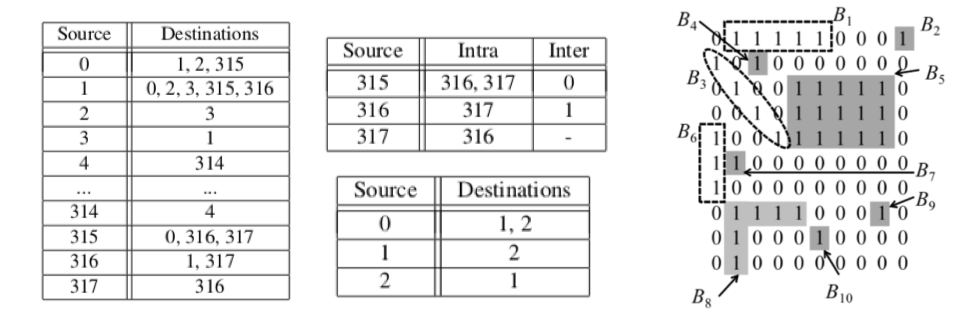
\includegraphics[scale=0.5]{ressources/image/inter_intra.png} 
					\caption{Exemple illustrant le principe de fonctionnement \citep{asano2008efficient}}
					\label{interIntra}
				\end{figure}
										Dans une méthode toute récente 
\newacronym{gcupmt}{GCUPMT}{Graph Compression Using Pattern Matching}			
			s'intitulant \gls{gcupmt}, Shah et Rushabh \citep{shah2018graph}  partitionnent les lignes de la matrice d'adjacence en plusieurs blocs ayant la même taille des motifs qui sont dans ce cas sous forme de vecteurs prédéfinies. Les blocs sont comparés avec l'ensemble des motifs ce qui entraîne , en cas de correspondance , le remplacement du bloc par un indicateur du motif précédé par un 1 indiquant que les bits suivants appartiennent à un indicateur de motif. Dans le cas contraire, les données brutes sont stockées directement précédées par un 0.
				
						%							\begin{landscape}
								\begin{table}
									\begin{tabular}{|c|c|c|c|c|c|c|c|c|c|c|c|c|}
										\hline
										\multirow{2}{*}[-25pt]{Article}  & \multicolumn{4}{c|}{Graphe en entrée} & \multicolumn{2}{c|}{Compression} & \multicolumn{2}{c|}{Structure en sortie}  & \multirow{2}{*}[-25pt]{Graphe de test} & \multirow{2}{*}[-25pt]{Résultat}  \\ \cline{2-11}
				& \rotatebox[origin=c]{90}{ Orienté }  & \rotatebox[origin=c]{90}{ Non orienté } & \rotatebox[origin=c]{90}{ Statique } & \rotatebox[origin=c]{90}{ Dynamique } & \rotatebox[origin=c]{90}{ Avec perte } & \rotatebox[origin=c]{90}{ Sans perte } & \rotatebox[origin=c]{90}{ Succincte } & \rotatebox[origin=c]{90}{ Structurelle }  & & \\ \hline				%%%%%%Fin du header
				
				\hline ECWG
 \citep{asano2008efficient}& \cmark & \cmark & \cmark & \xmark & \xmark &\cmark & \cmark & \xmark  &
										
	\begin{minipage}[t]{0.3\textwidth}
	uk-2002
    \begin{itemize}
    \item 18 millions de nœuds
    \item 298 millions liens\\
    
    \end{itemize}
  \end{minipage}	
										 & 76.1\%	\\
										
										\hline GCUPMT \citep{shah2018graph} & \cmark & \cmark & \cmark & \xmark & \xmark &\cmark & \cmark & \xmark & 
										
	\begin{minipage}[t]{0.3\textwidth}
	graphes avec :
    \begin{itemize}
    \item 8192 nœuds
    \\
    
    \end{itemize}
  \end{minipage}								 
			  & 70\%	\\

										\hline
									\end{tabular}
									\caption{Synthèse des méthode de compression par extraction de motifs basées vocabulaire exploitant les propriétés de la matrice d'adjacence.}									
									
								\end{table}
								
							\end{landscape}
					
				
				%%%%%%%%%%%%%%%%%%%%%%%%%%%%%%%%
				\subsection{Compression basée sur l'agrégation des motifs}
				
					Les méthodes de compression par extraction de motifs basées sur l'agrégation sont des méthodes   qui agrègent plusieurs nœuds ou liens d'un motif en un seul nœud, appelé super-nœud. Le graphe en sortie, dit super-graphe, devient dès lors plus simple et moins complexe offrant ainsi une aisance et une facilité de traitement, d'exploration et de visualisation. Nous présenterons dans ce qui suit les deux sous-classes de cette classe qui se distinguent selon que l'agrégation concerne les nœuds ou les liens.
					
					\begin{enumerate}[label=\alph*.]
				
					
					\item \subsubsection{Les méthodes de compression basées l'agrégation de nœuds}
					
					Les techniques de compression basées sur l'agrégation des nœuds des motifs sont des méthodes qui ont existé depuis plusieurs décennies offrant plusieurs avantages. 
					Elles visent à résumer le graphe initial en agrégeant les nœuds des motifs découvert dans le but de diminuer le nombre de nœuds existants  et d'offrir une meilleure visibilité et analyse du graphe. 
						
						Une première méthode de cette classe s'intitule Subdue \citep{ketkar2005subdue}. Elle effectue une recherche \textit{Branch\&Bound} qui commence à partir des sous-structures composées de tous les sommets avec des étiquettes uniques. Les sous-structures sont prolongées de toutes les manières possibles par un sommet et une arête ou par une arête afin de générer des sous-structures candidates. Subdue conserve les instances des sous-structures et utilise l'isomorphisme de graphe pour déterminer les instances de la sous-structure candidate. Les sous-structures sont ensuite évaluées en fonction de leur compression de la longueur de description (DL) du jeu de données. Cette procédure se répète jusqu'à ce que toutes les sous-structures soient prises en compte ou que les contraintes imposées par l'utilisateur ne soient plus vérifiées. A la fin de la procédure, Subdue indique les meilleures sous-structures de compression.
				Le système Subdue fournit également la possibilité d'utiliser la meilleure sous-structure trouvée lors d'une étape de découverte pour compresser le graphe d'entrée en remplaçant les instances de la sous-structure par un seul sommet et en effectuant le processus de découverte sur le  compressé. Cette fonctionnalité génère une description hiérarchique du jeu de données du graphe à différents niveaux d'abstraction en termes de sous-structures découvertes.\\
								Dans \citep{rossi2018graphzip}, les auteurs partent de l'observation que les graphes réels sont formés souvent de nombreuses cliques de grande taille. En utilisant ceci comme base, GraphZip décompose le graphe en un ensemble de grandes cliques, qui est ensuite utilisé pour compresser et représenter le graphe de manière succincte. 
					%							\begin{landscape}
								\begin{table}
									\begin{tabular}{|c|c|c|c|c|c|c|c|c|c|c|c|c|}
										\hline
										\multirow{2}{*}[-25pt]{Article}  & \multicolumn{4}{c|}{Graphe en entrée} & \multicolumn{2}{c|}{Compression} & \multicolumn{2}{c|}{Structure en sortie} & \multicolumn{2}{c|}{Complexité} & \multirow{2}{*}[-25pt]{Graphe de test} & \multirow{2}{*}[-25pt]{Résultat}  \\ \cline{2-11}
				& \rotatebox[origin=c]{90}{ Orienté }  & \rotatebox[origin=c]{90}{ Non orienté } & \rotatebox[origin=c]{90}{ Statique } & \rotatebox[origin=c]{90}{ Dynamique } & \rotatebox[origin=c]{90}{ Avec perte } & \rotatebox[origin=c]{90}{ Sans perte } & \rotatebox[origin=c]{90}{ Succincte } & \rotatebox[origin=c]{90}{ Structurelle } & \rotatebox[origin=c]{90}{ Temporelle} & \rotatebox[origin=c]{90}{ Spaciale} & & \\ \hline				%%%%%%Fin du header
				
				\hline Subdue
 \citep{ketkar2005subdue}& \xmark & \cmark & \cmark & \xmark & \xmark & \cmark & \xmark & \cmark	 & & &		
	\begin{minipage}[t]{0.3\textwidth}
	Composante chimique :
    \begin{itemize}
    \item 21 étiquettes
    \item 422 transactions\\
    
    \end{itemize}
  \end{minipage}	
										 & 16\%	\\
										
										\hline GraphZip \citep{rossi2018graphzip} & \xmark & \cmark & \cmark & \xmark & \xmark & \cmark & \xmark & \cmark & & & 
				Web-Google						
								 
			  & 19\%	\\

										\hline
									\end{tabular}
									\caption{Synthèse des méthodes de compression par extraction de motifs basées agrégation de nœuds.}									
									
								\end{table}
								
							\end{landscape}
					
					\item \subsubsection{Les méthodes de compression basées sur l'agrégation de liens}
						Les méthodes de compression par extraction de motifs basées sur l'agrégation de liens sont parmi les méthode les plus populaires. Leur objectif est de produire un graphe compressé à partir du graphe initial en remplaçant les liens denses du graphe par un nouveau super-nœud. Elles se divisent selon le principe en deux grandes classes: celles utilisant les règles de grammaire et celles utilisant des heuristiques de clustering. Nous détaillerons dans ce qui suit ces deux classes.
						
						\begin{enumerate}[label*=\arabic*.]
							\item \textbf{Les méthodes de compression basées sur les règles de grammaire}
							La classe des méthodes de compression basées sur les règles de grammaire est une généralisation d'une méthode de compression des dictionnaires s'intitulant Re-pair. Son principe de base consiste en la  recherche, à chaque itération, de la paire de symboles la plus fréquente dans une séquence de caractères et de la remplacer par un nouveau symbole, jusqu'à ce qu'il ne soit plus commode de les remplacer. Nous notons que dans ce cas le motif est sous forme de deux arêtes ayant un sommet en commun, nommé \textit{digraph}.
								
										Une première méthode suivant ce principe a été proposée dans \citep{claude2010fast} baptisée \textit{Approximate Re-pair}. Dans cette méthode un graphe G=(V,E) est représenté sous forme d'une sequence de caractères T: \begin{center}
		T=T(G)= $\overline{v_{1}}\ v_{1,1}\ ...\ v_{1,a}\ \overline{v_{2}}\ v_{2,1}\ ...\ v_{2,a_{2}} ... \overline{v_{n}}\ v_{n,1}\ ...\ v_{n,a_{n}}\ $						
\end{center}	
où $\overline{v_{i}}$ représente l'identificateur du sommet $v_{i}$. Elle procède en trois étapes essentielles expliquer dans l'algorithme \textbf{\ref{alg:re_pair}} .
	\begin{algorithm}
		\caption{Approximate Re-pair}
		\label{alg:re_pair}
		\begin{algorithmic}[1]
			\STATE \textbf{Calcule des fréquences:} T est parcourue séquentiellement et chaque pair $t_{i}t_{i+1}$ est ajoutée à un tableau de hachage H avec leur nombre d'occurrences. 
			\STATE \textbf{Recherche des k meilleurs paires:}  H est parcourue et les k paires les plus fréquentes sont retenues, en utilisant k pointeurs vers les cellules de H.
			\STATE \textbf{Le remplacement simultané:} les k paires identifiées dans l'étape précédente sont simultanément remplacées par un nouveau identifiant et une règle de production est ajoutée.
		\end{algorithmic}
	\end{algorithm}
	Lorsqu'il n'y a plus de paires à remplacer, Approximate Re-pair s'arrête donnant comme résultat un représentation compacte C de la chaine T. Pour finaliser le processus, tous les indicateurs de nœuds $\overline{v_{i}}$ seront supprimés de C. De plus, l'algorithme crée une table qui contiendra des pointeurs vers le début de la liste d'adjacence de chaque nœud dans C. Grâce à cette table l'algorithme pourra répondre aux requêtes de recherche de successeurs en un temps optimal.
								 %%%%exemple ???
									Dans un travail ultérieur \citep{claude2010extended} , les même auteurs s'intéressent aux requêtes de recherche des nœuds prédécesseurs et successeurs à partir du graphe compressé de \textit{Approximate Re-pair} directement. Il proposent alors de combiner leur méthode avec une représentation basée sur les relations binaires de \citep{barbay2006adaptive}. En effet, ce dernier consiste à représenter les listes d'adjacences à l'aide d'une représentation séquentielle permettant de rechercher les occurrences d'un symbole puis de rechercher les voisins inverses à l'aide de cette primitive. 
								
Claude et Ladra \citep{claude2011practical} partagaient les mêmes préoccupations des auteurs de la méthode précédente et ont proposé comme solution de combiner la méthode Re-pair avec la représentation k2-tree. Ils obtiennent alors une compression de 2,27 (pbe) sur le graphe UK2002, tout en conservant la possibilité d'interroger les voisins entrants et sortants \citep{maneth2015survey}.
							
								
	Une dernière méthode de cette classe s'instituant gRepair a été proposée dans \citep{maneth2018grammar}. Ce nouveau algorithme de compression détecte de manière récursive des sous-structures répétées et les représente via des règles de grammaire.  Des requêtes spécifiques telles que l'accessibilité entre deux nœuds ou des requêtes de chemin normal peuvent ainsi être évaluées en temps linéaire (ou en temps quadratique, respectivement), sur la grammaire, permettant ainsi des accélérations proportionnelles au taux de compression. La figure \ref{gRepair} présente le résultat de cette méthode sur un exemple. 
	
	\begin{figure}[h]
			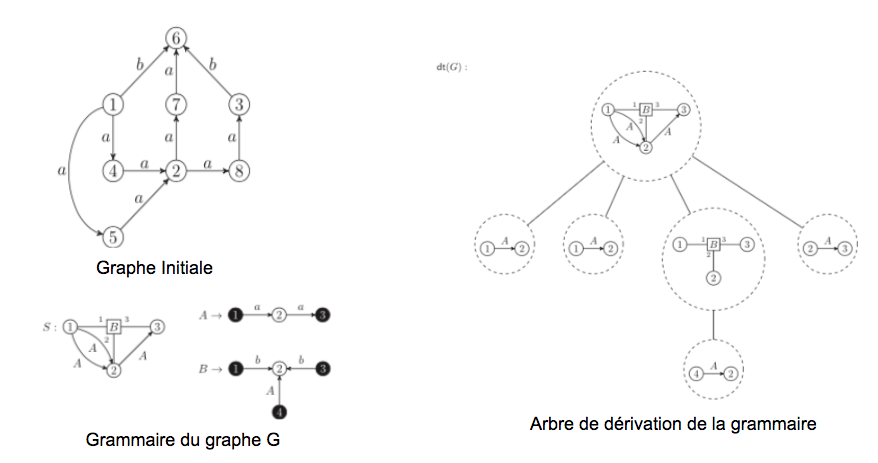
\includegraphics[scale=0.5,center]{./ressources/image/grepair.png}
			\caption[Exemple d'exécution de gRepair sur G.]{Exemple d'exécution de gRepair sur G.}
			\label{gRepair}
	\end{figure}
								%%%%exemple ???
							%															\begin{landscape}
								\begin{table}
									\begin{tabular}{|C{3cm}|c|c|c|c|c|c|c|c|c|c|c|c|}
										\hline
										\multirow{2}{*}[-25pt]{Article}  & \multicolumn{4}{c|}{Graphe en entrée} & \multicolumn{2}{c|}{Compression} & \multicolumn{2}{c|}{Structure en sortie} & \multicolumn{2}{c|}{Complexité} & \multirow{2}{*}[-25pt]{Graphe de test} & \multirow{2}{*}[-25pt]{Résultat (bits/lien)}  \\ \cline{2-11}
				& \rotatebox[origin=c]{90}{ Orienté }  & \rotatebox[origin=c]{90}{ Non orienté } & \rotatebox[origin=c]{90}{ Statique } & \rotatebox[origin=c]{90}{ Dynamique } & \rotatebox[origin=c]{90}{ Avec perte } & \rotatebox[origin=c]{90}{ Sans perte } & \rotatebox[origin=c]{90}{ Succincte } & \rotatebox[origin=c]{90}{ Structurelle } & \rotatebox[origin=c]{90}{ Temporelle} & \rotatebox[origin=c]{90}{ Spaciale} & & \\ \hline				%%%%%%Fin du header
				
				\hline Approximate Re-pair
   \citep{claude2010fast}& \cmark & \xmark & \cmark & \xmark & \xmark &  \cmark & \cmark & \xmark	 & & &		
	\begin{minipage}[t]{0.3\textwidth}
	uk-2002 :
    \begin{itemize}
    \item 18 millions de nœuds
    \item 298 millions de liens\\
    
    \end{itemize}
  \end{minipage}	
										 & 4.23	\\

										\hline Approximate Re-pair \citep{claude2010extended} & \cmark & \xmark & \cmark & \xmark & \xmark & \cmark & \cmark & \xmark  & & & 
										\begin{minipage}[t]{0.3\textwidth}
	uk-2002 :
    \begin{itemize}
    \item 18 millions de nœuds
    \item 298 millions de liens\\
    
    \end{itemize}
  \end{minipage}	 & 3.98 \\ 
  			\hline gRe-pair \citep{maneth2018grammar} & \cmark & \cmark & \cmark & \xmark & \xmark & \cmark & \cmark & \xmark & & &
  				\begin{minipage}[t]{0.3\textwidth}
  			NotreDame :
    \begin{itemize}
    \item 325 milles de nœuds
    \item 1M de liens\\
  		\end{itemize}
  \end{minipage}		
  			& 4.84 \\\hline
									\end{tabular}
									\caption{Synthèse des méthodes de compression par extraction de motifs basées agrégation de liens en utilisant les règles de grammaire.}									
									
								\end{table}
								
							\end{landscape}
							\item \textbf{Les méthodes de compression basées sur des heuristiques de clustering} 				
							
							Les méthodes de compression appartenant à cette classe sont des méthodes basées sur la recherche des sous-graphes denses (ayant des nœuds fortement connectés). Elles sont destinées principalement aux graphes du Web et les graphes des réseaux sociaux dans le but de faciliter leur exploration et analyse.
								
									%-----------------Aggregation des liens ----------%
				\citep{buehrer2008scalable} ont exploité l'existence de plusieurs ensembles de pages web qui ont les mêmes liens sortants. S'intitulant  
\newacronym{vnm}{VNM}{Virtual Node Miner}				
				\gls{vnm}, leur approche est basée sur la réduction du nombre de liens en créant des nouveaux sommets virtuels qui sont ajoutés au graphe. Soit G = (V,E) un graphe orienté, l'algorithme proposé se compose de deux phases essentielles :
				\begin{enumerate}
				
				
					\item \textbf{Phase de Clustering :}
					
					Le but de cette première étape est de contourner la tâche presque impossible d'extraction simultanée de centaines de millions de points de données en groupant d'abord les sommets similaires dans le graphes dans des clusters. 
				Pour cela k fonctions de hachage indépendantes sont utilisées pour obtenir une matrice de taille V * k. Par la suite, les lignes de la matrice  sont triées lexicographiquement
				%Ce tri est assez rapide car il ne nécessite que O (2V log V) en mémoire à la fois, ce qui tient dans la RAM (ou nous le faisons en minant le graphique en morceaux). 
				et elle est parcourue colonne par colonne en regroupant les lignes ayant la même valeur. Lorsque le nombre total de lignes chute au-dessous d'un seuil ou que le bord de la matrice de hachage est atteint, les identifiants des sommets associés aux lignes sont renvoyés au processus d'extraction (Phase 02). 
					
					\item \textbf{Phase d'Extraction de Motifs :}				Le but de cette étape est de localiser des sous-ensembles communs de liens sortants dans les sommets donnés. 
				Ainsi les ensembles plus grands et fréquents présentent un intérêt, car ils peuvent représenter des motifs plus pertinents et une meilleure compression. En effet, les performances de compression d'un motif sont calculés en fonction de sa fréquence dans la liste d'adjacence, et de sa taille qui est le nombre de liens qu'il contient (Formule \ref{eqcompperf}).
				%%% Formule
				\begin{equation}
				Compression(P)=(P.fréquence-1)(P.taille-1)-1
				\label{eqcompperf}
				\end{equation}
				Afin d'extraire ces motifs, \gls{vnm}  utilise une heuristique gloutonne. Cette heuristique procède comme suit :
				\begin{enumerate}
				\item Extraire un histogramme des identifiants de liaison sortante à partir de la liste d'adjacence des sommets données.
				\item Les listes sont réorganisées dans l'ordre décroissant des fréquences des liens sortants en éliminant ceux qui apparaissent une seul fois uniquement.
				\item Chaque lien sortant est ajouté à un arbre de préfixes avec l'ensemble trié de ces extrémités initiales selon leurs identifiants. 
				\item L'arbre est par la suite parcouru afin d'identifier les motifs qui maximisent la formule de performance de la compression (Formule \ref{eqcompperf}). Ces motifs sont ensuite convertis en nœuds virtuels et les identificateurs de sommets de leurs listes sont remplacés par les ids des nœuds virtuels dans la liste d'adjacence.
				\end{enumerate}
				 
				\end{enumerate}
				
				L'algorithme est appliqué jusqu'à ce que la réduction n'apporte pas un gain significatif. La figure \ref{VNM_exemple} illustre le principe de fonctionnement de cette méthode sur un exemple.
				
				
			%%%%		Inclure un exemple 
		
		
			\begin{figure}[!h]
			\centering
			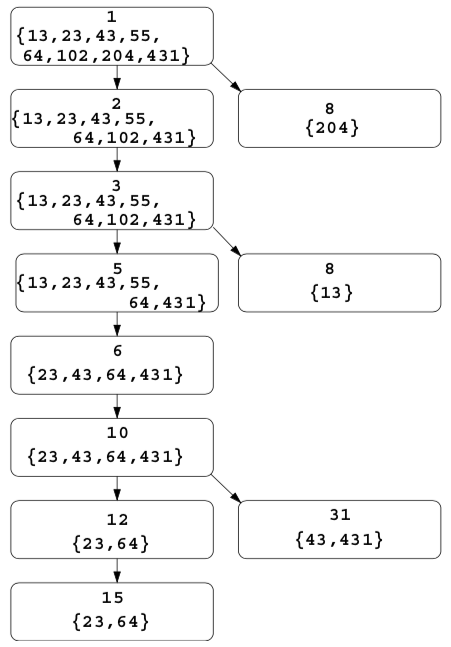
\includegraphics[scale=0.3,center]{./ressources/image/VNM_exemple.png}
			\caption[Exemple d'exécution de VNM .]{Exemple d'exécution de VNM.}
			\label{VNM_exemple}
	\end{figure}
								\newpage	
	Une variante de \gls{vnm} , 
	\newacronym{dsm}{DSM}{Dense SubGraph Mining}	
	\gls{dsm}, a été proposée par Hernandez et Navarro \citep{hernandez2014compressed}. Comme première contribution, ils augmentent les types de structures découvertes dans la phase de clustering pour englober aussi: les cliques, les bi-cliques. L'extraction de motifs cette fois-ci n'est pas basée sur un parcours des feuilles vers la racine mais l'inverse où  l'ensemble des sommets finaux des liens du motifs est constitué des étiquettes des nœuds de l'arbre inclues dans le chemin de la racine vers la feuille et  les sommets initiaux sont la liste des sommets inclus dans le nœud feuille. 
				%%Noublie pas revient vers la source 
				Leur deuxième contribution consiste en une hybridation dans le but de représenter le graphe en sortie à l'aide de structures compactes. Une première approche proposée est d'utiliser les  k2-trees \citep{brisaboa2009k}  qui donnent la représentation la plus compacte.  
				La deuxième hybridation consiste en une nouvelle structure proposée par les auteurs.\\
				
				
				
				\begin{figure}[!h]
					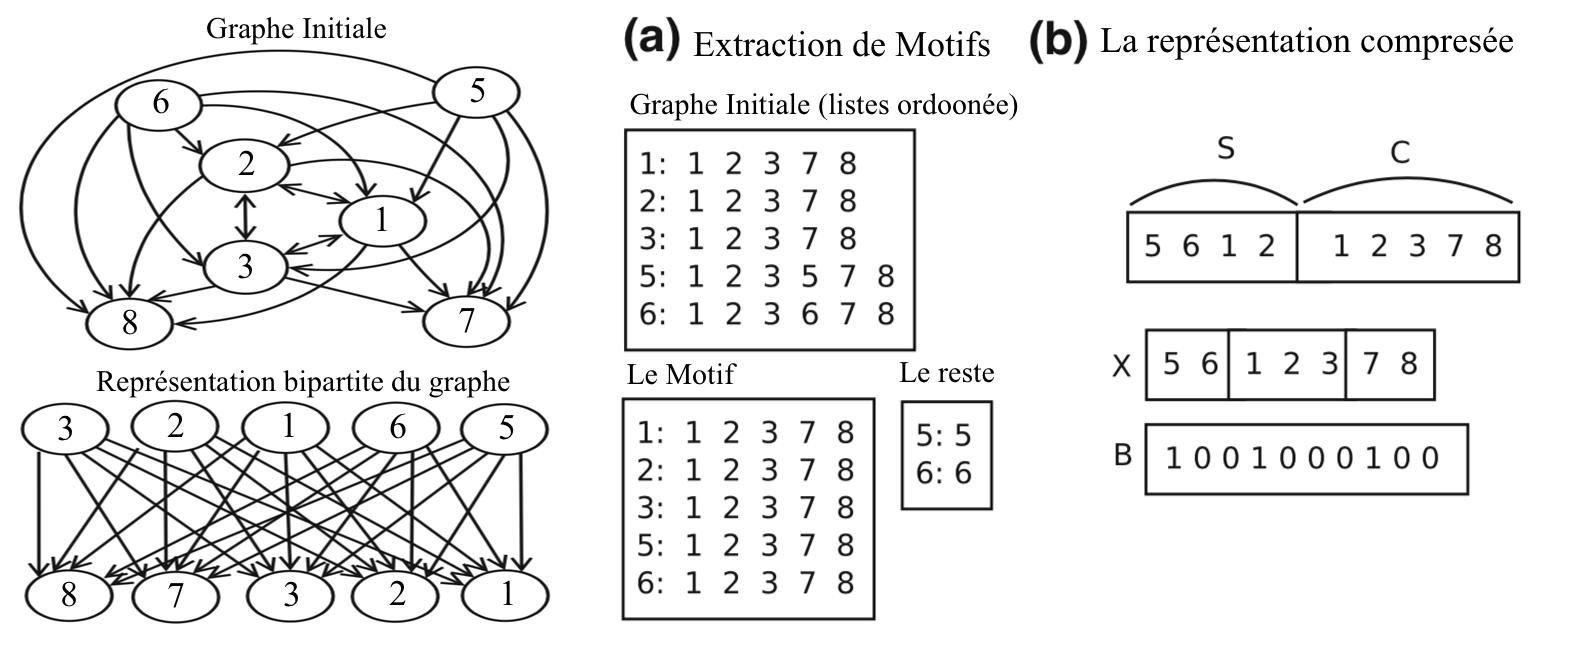
\includegraphics[scale=0.23]{ressources/image/VNM2_exemple.png} 
					\caption{Exemple d'exécution de DSM}
					\label{SDM}
				\end{figure}
					
						
						\end{enumerate}	
					
					\end{enumerate}
						
						\subsection{Synthèse des méthodes de compression par extraction de motifs }

	Durant les sections précédentes nous avons expliqué de manière générale les fondements de base de chaque sous-classe de la classe des méthodes de compression par extraction de motifs ainsi que le principe de fonctionnement de leurs méthodes. 
	
	Nous regroupant dans le tableau \ref{enfin} les différentes caractéristiques des méthodes de ces sous-classes. Nous observons qu'elles sont toutes sans perte et destinées aux graphes statiques, à l'exception de la classe des méthodes de compression Basées vocabulaire en utilisant les méthodes de clustering qui contiennent des méthodes de compression supportant les graphes dynamiques. On remarque aussi que la majorité des méthodes de compression par extraction de motifs fournissent en sortie une représentation succincte. Le tableau \ref{enfin} contient aussi un résumé sur les résultats de l'application de ces méthodes sur des graphes de tests issues de domaines hétérogènes.
	
			
			

\begin{landscape}
								\begin{table}
								%\renewcommand{\arraystretch}{2}
									\begin{tabular}{|c|C{5.5cm}|c|c|c|c|c|c|c|c|C{2.5cm}|c|}
										\hline
										\multirow{2}{*}[-25pt]{Classe} & \multirow{2}{4cm}[-25pt]{Méthode}  & \multicolumn{4}{c|}{Graphe en entrée} & \multicolumn{2}{c|}{Compression} & \multicolumn{2}{c|}{Structure en sortie}  & \multirow{2}{*}[-25pt]{Graphe de test} & \multirow{2}{*}[-25pt]{Résultat}  \\ \cline{3-10}
				& & \rotatebox[origin=c]{90}{ Orienté }  & \rotatebox[origin=c]{90}{ Non orienté } & \rotatebox[origin=c]{90}{ Statique } & \rotatebox[origin=c]{90}{ Dynamique } & \rotatebox[origin=c]{90}{ Avec perte } & \rotatebox[origin=c]{90}{ Sans perte } & \rotatebox[origin=c]{90}{ Succincte } & \rotatebox[origin=c]{90}{ Structurelle }  & & \\ \hline	 \hline			%%%%%%Fin du header
										
										 \multirow{4}{4cm}{Basée vocabulaire en utilisant  les méthodes de clustering}& VoG \citep{koutra2015summarizing} & \xmark & \cmark & \cmark & \xmark & \xmark & \cmark & \cmark & \xmark  & 
	
	
	Enron									 
			  & 75\%	\\ \cline{2-12}

										 & VoG-Overlapp \citep{liu2015empirical}& \xmark & \cmark & \cmark & \xmark & \xmark &\cmark & \cmark & \xmark  & Enron							 & 75\%	\\  \cline{2-12}
										 & TimeCrunch \citep{shah2015timecrunch}& \xmark & \xmark & \cmark & \cmark & \xmark &\cmark & \cmark & \xmark & 

	
	Enron			&74\%	\\  \cline{2-12}
										 & CanDenSe \citep{liu2018reducing}&     \xmark & \cmark & \xmark & \cmark & \xmark  &\cmark & \cmark & \cmark & Enron									
										 &	 78\%\\ \hline \hline
										 
										 \multirow{2}{4cm}{\footnotesize{Basée vocabulaire en utilisant  les propriétés de la matrice d'adjacence}}&  ECWG
 \citep{asano2008efficient}& \cmark & \cmark & \cmark & \xmark & \xmark &\cmark & \cmark & \xmark  &
	uk-2002	 & 76.1\%	\\  \cline{2-12}
	
	& GCUPMT \citep{shah2018graph} & \cmark & \cmark & \cmark & \xmark & \xmark &\cmark & \cmark & \xmark & 
	graphes 8192 nœuds
							 
			  & 70\%	\\ \hline \hline
			  
			\multirow{2}{4cm}{\small{Basée Agrégation de nœuds des motifs}} & Subdue
 \citep{ketkar2005subdue}& \xmark & \cmark & \cmark & \xmark & \xmark & \cmark & \xmark & \cmark &		
	Graphe des composantes chimiques
										 & 16\%	\\ \cline{2-12}
										 
										 & GraphZip \citep{rossi2018graphzip} & \xmark & \cmark & \cmark & \xmark & \xmark & \cmark & \xmark & \cmark & 
				Web-Google						
								 
			  & 19\%	\\ \hline \hline
			  
			  \multirow{3}{4cm}{Basée Agrégation de liens des motifs en utilisant les règles de grammaire} & Approximate Re-pair
   \citep{claude2010fast}& \cmark & \xmark & \cmark & \xmark & \xmark &  \cmark & \cmark & \xmark	 &		
	uk-2002 & 4.23	\\ \cline{2-12}
	 &  Approximate Re-pair \citep{claude2010extended} & \cmark & \xmark & \cmark & \xmark & \xmark & \cmark & \cmark & \xmark  & 
	uk-2002	 & 3.98 bpe \\	\cline{2-12}
	
	& gRe-pair \citep{maneth2018grammar} & \cmark & \cmark & \cmark & \xmark & \xmark & \cmark & \cmark & \xmark &
  			
  			NotreDame
  			& 4.84 bpe \\ \hline \hline
  			  \multirow{2}{4cm}{\small{Basée Agrégation de liens des motifs et les méthodes de clustering}}& VNM
 \citep{buehrer2008scalable}& \cmark & \xmark & \cmark & \xmark & \xmark & \cmark & \xmark & \cmark &		
	uk-2002 	 & 1.95 bpe \\ \cline{2-12}
	& DSM \citep{hernandez2014compressed} & \cmark & \xmark & \cmark & \xmark &  \xmark & \cmark & \cmark & \cmark  & 
				
	uk-2002 					 
			  & 1.53 bpe	\\
									\hline	 
									\end{tabular}
									\caption{Synthèse des méthodes de compression par extraction de motifs.}
									\label{enfin}									
									
								\end{table}
								
							\end{landscape}
							
							

							
							
								
		\section{Conclusion}
	
De nos jours, les graphes sont omniprésents. Cependant, leur taille présente un obstacle presque insurmontable à la compréhension du caractère essentiel des données. D'où la nécessité de la compression qui permet de réduire la taille des graphes tout en gardant le caractère utile de l'information incluse dans ces derniers.

Nous avons étudié dans ce chapitre différentes méthodes de compression de graphes dans le but d'établir une classification des méthodes basée sur deux approches : l'extraction de motifs et les arbres k2-trees. Nous nous sommes appuyer pour cela sur le principe de fonctionnement de chacune d'elles. Nous  proposons six classes de méthodes :

\begin{enumerate}[label=\roman*]
\item  Les méthodes de compression par les k2-trees
	\item  Les méthodes de compression par extraction de motifs basées vocabulaires en utilisant des méthodes de clustering.
	\item  Les méthodes de compression par extraction de motifs basées vocabulaires exploitant les propriétés de la matrice d'adjacence.
	\item  Les méthodes de compression par extraction de motifs basées agrégation de nœuds.
	\item  Les méthodes de compression par extraction de motifs basées agrégation de liens en utilisant des règles de grammaire.
	\item  Les méthodes de compression par extraction de motifs basées agrégation de liens en utilisant des heuristiques de clustering.
\end{enumerate}
	
Nous avons présenté le principe de fonctionnement des méthodes relatif à chaque classe tout en comparant leurs caractéristiques. 
 Ces classes diffèrent les unes des autres dans leurs fondements théoriques, le type de compression considéré, la complexité des algorithmes, les objectifs et les domaines d'application. 
 Dans le tableau \ref{comgen} , nous allons essayer de synthétiser les principales différences et similitudes entre les deux approches, compression par extraction de motifs et compression par les arbres k2-trees, que nous avons pu constater à travers notre recherche bibliographique. Ils ont un fort impact sur le choix de la méthode de compression du moment qu'ils ont une influence directe sur les performances.
 
\begin{table}[H]
\begin{tabular}{|c|p{6cm}|p{4cm}|}

\hline & \begin{center}
\textbf{$k^2$-trees}
\end{center}     &  \begin{center} \textbf{Extraction de motifs} \end{center}  \\
										
										
\hline Type de compression & toujours sans perte & toujours sans perte \\
\hline Structure en sortie & Toujours succincte & Peut être succincte où structurelle où les deux en même temps\\

\hline technique utilisée & exploitation de la matrice d'adjacence du graphe & exploitation des motifs fréquents dans le graphe\\

\hline Dépendance & Dépend du paramètre k & Dépend selon la méthode de l'algorithme de clustering ou du vocabulaire de motifs utilisé  \\

\hline Objectif & 
\begin{minipage}[t]{0.35\textwidth}
  			Compression,\\
  			Réduire l'espace de stockage et le temps de parcours\\
  \end{minipage}
  &
  \begin{minipage}[t]{0.25\textwidth}
  			- Compression,\\
  			- Réduire l'espace de  stockage et le temps de parcours,\\
  			- Extraire les informations pertinentes, \\
  			- Visualisation \\
  \end{minipage}
  \\
  \hline Domaine d'application & tous les domaines & tous les domaines \\
  \hline Type de graphes supporté & 
 \begin{minipage}[t]{0.25\textwidth}
  			- Statique orienté,\\
  			- Attribué,\\
  			- Dynamique, \\
  \end{minipage}  
  &  \begin{minipage}[t]{0.25\textwidth}
  			- Statique (orienté et non orienté),\\
  			- étiqueté,\\
  			- Dynamique, \\
  \end{minipage}  
  \\ \hline
\end{tabular}
									\caption{Comparaison entre les méthodes basées sur$k^2$-trees et basées sur l'extraction de motifs.}									\label{comgen}
									
								\end{table}
								
				
	

	
	
	


	
	


\part{Contribution}

%
Comme on vient de voir dans les chapitres précédents, de nombreux phénomènes dans des contextes très variés peuvent être représenter par des graphes. Citons en particuliers les réseaux sociaux qui nous attirent vu leur importance et leur fort impact sur la vie réel. En effet, trois quarts des personnes connectées à internet utilisent les réseaux sociaux. Ils rassemblent aujourd'hui 3,169 milliards d'utilisateurs actifs, voir 40\% de la population sur terre, avec 11 personnes s'inscrivant chaque seconde sur Facebook, Twitter et autres
\footnote{https://bfmbusiness.bfmtv.com/hightech/la-moitie-de-la-population-mondiale-est-connectee-a-internet-1361933.html}. De ce fait, deux constats s'impose: le premier est l'incapacité des graphes statiques à décrire certaines situations de la vie réelle et leur évolution dans le temps, le deuxième est la montée en flèche de la quantité et l'hétérogénéité des informations modélisées par ces réseaux et qui rendent presque impossible tout traitement. D'où le besoin croissant de méthodes de compression de graphes dynamiques. 

Nous nous sommes aussi intéressées dans ce travail à un autre enjeu important qui est la recherche de motifs et particulièrement les clique et les noyaux bipartie qui sont fréquents dans les réseaux faisant abstraction à des situations réelles importantes dans le processus de prise de décision. Nous citons par exemple, les attaquants de réseaux de botnet formant un noyau bipartie avec leurs victimes pendant la durée d'une attaque, les membres de la famille se liant comme une clique au cours d'une période difficile, ou les collaborations de recherche s'étant créées et qui disparaissent au cours des années.

%Quoiqu'il existe de nombreuses techniques de compression efficaces adaptées au contexte statique, rares sont ceux qui proposent une contrepartie dynamique, ce qui nous amène à s'intéresser particulièrement à ce type de graphes toujours en cours d'évolution. 

Nous allons dans cette partie proposer une nouvelle méthode \gls{ddsm} basée sur deux approches existantes que nous avons étudié dans notre état de l'art. Notre but principal est de développer une technique de compression compétitive pour les graphes des réseaux sociaux dans un contexte dynamique en se basant sur l'extraction de motifs. Pour accomplir ce travail nous nous sommes appuyés sur ces deux méthodes :
\begin{itemize}
\item Exploiter la structure de données compressée proposée dans \gls{dsm} \citep{hernandez2014compressed} qui permet de représenter les sous-graphes denses comme les cliques, les quasi-cliques, noyaux bipartis. Nous avons opté pour cette structure car en l'appliquant sur les réseaux sociaux, elle donne de bons résultats en matière d'espace et de temps de requêtes.  
\item Adopter les signatures temporelles utilisées dans TimeCrunch \citep{shah2015timecrunch} pour décrire le comportement des sous-graphes dans le temps. Nous avons utilisé ces signatures car elles englobent tous les types de comportements temporels d'un motif dans un graphe dynamique.
\end{itemize}	
%Nous allons dans cette partie présenter notre méthode théoriquement : principe général, structure utilisée et un pseudo code.	
		
		\subsubsection{Formulation du problème}
		Dans cette section, nous allons définir le problème de base auquel notre méthode convient tout en définissant le cadre dans lequel elle peut être appliquée. 
		
		Nous considérons les graphes orientés dynamiques $\displaystyle{G=\bigcup_{t_{i}}G_{t_{i}}(V,E_{t_{i}})}\ \ 1 \preceq i \preceq t$ où $G_{t_{i}}$ = G a l'instant $t_{i}$ et un ensemble de signatures temporelles. En d'autre termes, nous considérons des captures du graphe à des instants différents $t_{i}$ et un ensemble de descripteurs de comportement temporel des sous-graphes des différents $G_{t_{i}}$. Le problème peut ainsi être formulé:
		
			\textit{\textbf{Problème:}
		Trouver, à partir d'un graphe dynamique G et un lexique de signatures temporelles, la plus petite description du graphe initial en termes de ses sous structures les plus denses et leur comportement temporel, en offrant la possibilité de manipuler le graphe, d'extraire les voisins directs d'un nœud à un instant donné et d'extraire les sous-graphes au besoin. }

		\subsubsection{Principe général}
			Notre méthode s'intitule DDSM pour \textit{Dynamic Dense Substructure Mining}. Elle représente une généralisation du travail de Hernandez et Navarro \citep{hernandez2014compressed} pour le cas des graphes dynamiques qui sont de nos jours omniprésents.
			
			%Pour mieux expliquer notre méthode nous allons tout d'abord commencer par décrire les structures que nous allons utiliser. Nous enchainons par la suite  avec le pseudo algorithme détaillant les étapes essentielles de notre méthode et nous conclurons en expliquant comment les algorithmes proposés dans \citep{hernandez2014compressed} de manipulation des graphes peuvent être généralisés dans notre cas.
			%\subsection{Description conceptuelle}
			
			La codification du graphe en sortie doit respecter les contraintes du problème tout en réduisant un maximum d'espace mémoire. Pour cela, Nous proposons d'étendre la codification proposée dans \citep{hernandez2014compressed} pour le cas des graphes dynamiques en rajoutant une information temporelle. 
			
			Une fois les sous-structures identifiées, Hernandez et al. \citep{hernandez2014compressed} proposent de représenter chacune d'elles avec trois composantes: la première contenant les sommets ayant uniquement des arêtes sortantes, la deuxième contenant les sommets ayant des arêtes entrantes et sortantes et la troisième contenant les sommets ayant uniquement des arêtes entrantes. Pour pouvoir identifier les différentes composantes, ils associent un vecteur binaire à cette représentation marquant par un 1 le début de chacune des trois composantes (voir figure \ref{SDM}).
			
			Notre première contribution consiste en l'extension de cette structure. En effet, nous suggérons de représenter chaque sous structure avec non pas trois composantes mais quarte composantes. Les trois premières étant les même que dans \citep{hernandez2014compressed}, la quatrième représente l'information temporelle. Cette dernière peut avoir cinq formats (voir section \ref{par:TimeCrunch}) dont nous résumons la représentation proposée pour chacune dans le tableau \ref{tab:signtmp}.
			
			\begin{table}[h]
			\label{tab:signtmp}
			\begin{center}
			\begin{tabular}{|r|l|}
			\hline Signature temporelle & Représentation	
			\\\hline constante & 0	
			
			\\\hline OneShot & 1 $t_{1}$	
			
			\\\hline ranged & 2	$t_{1}\ t_{2}$	
			
			\\\hline periodic & 3  $T$	
			
			\\\hline flikering & 4 $t_{1}\ t_{2}\ ...\ t_{n}$	
			
			\\\hline			
			\end{tabular}
			\end{center}
			
			 \caption{\small {Les types de signatures temporelles et leurs représentations, $t_{i}$	 représentent les timestamps et T représente la période.}}
			\end{table}
			
			Nous représentons G donc comme un ensemble de sous-graphes temporels denses. Cependant, pour obtenir une compression sans perte, nous devons aussi garder l'erreur modélisant l'ensemble d'arêtes restantes dans chaque $G_{t_{i}}$. Nous proposons pour cela d'utiliser une des structures dynamiques des k2-trees qui nous permettra d'interroger le graphe de manière simple et efficace.
			
			%\subsection{Notre méthode : DDSM}
			 Nous visons à travers la méthode que nous proposons d'exprimer le graphe en entrée avec ses sous-structures les plus denses et leur comportement temporel réduisant ainsi sa taille et offrant la possibilité d'effectuer les traitements dans un temps meilleur. Nous avons structuré notre algorithme sous forme de trois (03) étapes essentielles, chacune servant d'entrée pour l'étape suivante.
			 
			 En premier lieu, nous appliquons la découverte des sous-graphes les plus denses. Pour effectuer cela de manière efficace, nous suggérons d'utiliser l'approche proposée dans \citep{hernandez2014compressed} parallèlement sur chaque capture $G_{t_{i}}$ de G. Nous allons donc considérer les listes d'adjacences pour chaque $G_{t_{i}}$ où des fonctions de hachage sont calculées pour chaque sommet. Une arborescence est ensuite construite pour chaque ensemble de sommets ayant les même valeurs de hachages et qui permettra d'extraire les sous-structures denses du graphe à travers un parcours de la racine vers les feuilles. Dans une deuxième phase, nous effectuons une comparaison entre les sous-structures découvertes dans des timestamps différents afin de lui associer la signature appropriée. Durant cette étape, nous tolérons un certains seuil d'erreur qui sera inclus dans la représentation de l'erreur. Une dernière phase consiste en la codification du graphe en utilisant le codage proposé dans la section précédente pour chaque sous-structure de la phase (02). Nous concaténons par la suite ces représentations pour obtenir une seule représentation concise du graphe initial en termes de ses structures les plus denses. 
			L'algorithme \ref{alg:DDSM} résume les trois principales étapes de notre méthode.
			\begin{algorithm}
					\label{alg:DDSM}
					\caption{DDSM}
					\label{Pseudo Algorithme de la méthode proposée (DDSM)}
				\begin{algorithmic} [1]
					\STATE \textbf{Génération des sous structures candidates: }Génération de sous-graphes, principalement les sous-graphes bipartis et les cliques.
					
					\STATE  \textbf{Étiquetage de sous-structures: }Associer chaque sous-structure à une signature temporelle décrivant son comportement.
					
					\STATE \textbf{Codification du graphe compressé: }Codifier les sous-structures étiquetées de l'étape (02) en utilisant les structures de la section précédente.
				\end{algorithmic}
			\end{algorithm}
			
			Pour les algorithmes de parcours et d'extraction de voisins, tous les algorithmes proposés dans \citep{hernandez2014compressed} peuvent être généralisés sur notre structure. En effet, le seul changement consiste en la  prise en compte de l'information temporelle dans l'incrémentation des indices de parcours. De ce fait, nous pensons que notre méthode peut offrir un très bon compromis entre l'espace mémoire et le temps d'accès des traitements dans le cas des graphes dynamiques. 
			
		%\subsubsection{Conclusion}
	%Dans ce chapitre, nous avons abordé le problème de compression des graphes dynamiques par extraction de motifs. Nous avons formalisé le problème de compression d'un graphe dynamique en se basant sur les sous-graphes denses temporelles qui le composent. Pour faire face à ce problème nous avons présenté une nouvelle méthode hybride intitulée DDSM, elle combine deux méthodes de la littérature que nous avons jugé efficaces. Notre prochain but est de tester cette méthode en la comparant avec les méthodes existantes.   

	

\chapter{Conception}
	\section{Introduction}
	
	La réalisation de l'étude bibliographique dans le précédent chapitre, nous a initié au domaine de compression en général, et nous a permis d'approfondir nos connaissances dans le domaine de compression des graphes. Nous avons pu voir en détails les caractéristiques de plusieurs méthodes de compression s'inscrivant dans les deux classes de méthodes de compression: celles basées sur l'extraction de motifs et celles basées sur les arbres $k^2$-trees. La vocation de ce travail est d'enrichir un projet existant en l'étendant avec deux moteurs de compression qui regroupent différentes stratégies des deux classes étudiées. La réalisation de ces deux moteurs permettra de comparer entre ces stratégies et d'avoir une idée plus claire sur leurs performances dans différents scénarios.
	
	Dans ce chapitre, nous présenterons les détails de la conception des deux moteurs. Nous allons, dans un premier temps, présenter leur principe de fonctionnement tout en mettant l'accent sur les différents modules qui les constituent. Nous expliquerons juste après notre deuxième contribution qui consiste en une nouvelle  méthode de compression destinée aux graphes dynamiques.
	

	\section{$k^2$-GraCE : }
	\label{k2}

Dans cette section, nous présenterons  notre premier moteur baptisé \gls{$k^2$-GraCE}. Il consiste en un moteur de compression des graphes par les arbres $k^2$-trees qui exploitent les propriétés de localité et de similarité dans les graphes du web. 

		\subsection{Principe de fonctionnement :}
		
	Le moteur $k^2$-GraCE a été conçu pour permettre la compression de graphes statiques ou dynamiques et orientés ou non orientés. Il se base sur les travaux de Brisaboa et al. \citep{brisaboa2009k}. Il offre la possibilité de construire le graphe compressé à partir de la matrice d'adjacence, de la liste d'adjacence ou du graphe directement. Il permet aussi dans le cas des graphes dynamiques de réduire davantage la taille de l'arbre en le construisant n'ont pas à partir de la matrice d'adjacence initiale mais en calculant une matrice de différence entre les instants $t_i$. 
	
	
$k^2$-GraCE est un moteur de compression sans perte de données. En effet, il construit en sortie un arbre $k^2$-tree incluant toute information présente dans le graphe initial. Cette information est représentée sous forme de deux chaines binaires. Le processus de compression d'un graphe de données par le moteur $k^2$-GraCE passe par les étapes suivantes :
\begin{enumerate}
\item Lecture et structuration du graphe de données en entrée 
\item Pré-traitement : cette étape est optionnelle, elle ne figure pas dans l'algorithme de base. 
\item Construction récursive de l'arbre k2-tree à partir de la matrice d'adjacence (la liste d'adjacence ou du graphe directement) et la concaténation des différents niveaux dans une première chaine T, à l'exception du dernier niveau qui sera stocké dans une deuxième chaine L.

\item Écriture du graphe compressé sur le fichier de sortie.
\end{enumerate}

Nous illustrons ces phases par la figure \ref{k2grace} qui donne une vue globale sur le principe de fonctionnement de ce moteur.


\begin{figure}[H]
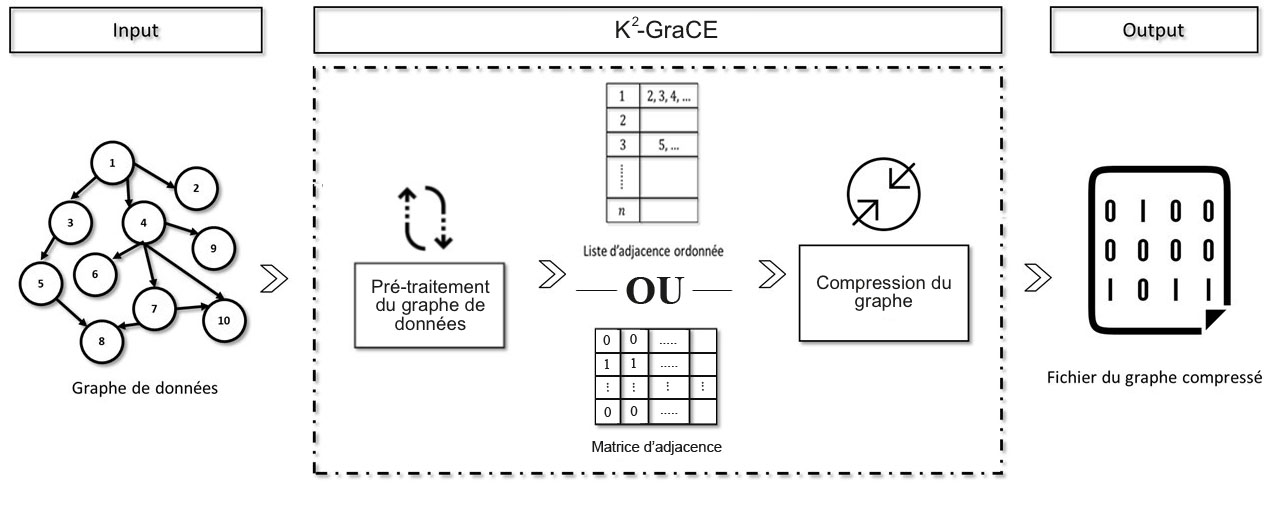
\includegraphics[scale=0.48]{./ressources/image/ograce.jpg}
\caption[Principe de fonctionnement du moteur $k^2$-GraCE]{Principe de fonctionnement du moteur $k^2$-GraCE.}
			\label{k2grace}
\end{figure}
Après avoir expliquer de manière générale le principe de fonctionnement du moteur $k^2$-GraCE, nous présenterons dans ce qui suit les détails des deux phases : la phase de pré-traitement et la phase de compression (construction de l'arbre). Nous allons tout d'abords commencer par présenter les notations et opérations de bases qui seront utilisées par la suite. Nous enchainerons par les différents algorithmes de construction selon le type de graphe en entrée.
		
		\subsection{Paramètre et notations :}
				
		\begin{table}[H]
		\centering
		\begin{tabular}{|c|L{12cm}|}
		\hline Paramètre & Signification \\ \hline\hline 
		$G$ & Graphe de données \\ \hline
		$M$ & Matrice d'adjacence du graphe G\\ \hline
		$List$ & Liste d'adjacence du graphe G\\ \hline
		$A$ & L'arbre $k^2$-tree \\\hline
		$T$ & Le nombre d'instants dans lesquels le graphe a été capturé \\\hline
		$h$ & La hauteur de l'arbre $k^2$-tree \\ \hline
		$N$ & Nombre de nœuds dans le graphe \\ \hline
		$k$ & Paramètre déterminant le nombre de fils dans l'arbre $k^2$-tree\\ \hline
		: & opérateur de concaténation \\ \hline
		rank($T,i$) &  Fonction calculant le nombre de 1 existant dans le tableau binaire $T$ dans l'intervalle des indices [$1,i$] \\ \hline
		\end{tabular}
		\caption{Tableau des notations et paramètres du moteur $k^2$-GraCE.}	
		\label{notk2grace}		
	\end{table}
	
		\subsection{Conception Modulaire:}
		
		Dans cette partie, nous détaillerons chaque phase du moteur $k^2$-GraCE. Nous commencerons par présenter les différentes techniques de pré-traitement 
		que nous voulons utiliser avec notre moteur. Nous expliquerons par la suite le processus de compression pour chaque type de graphe supporté par le moteur $k^2$-GraCE. %et nous allons aussi fournir les différents algorithmes d'extraction de voisins en Annexe \ref{k2_annexe}. 
		
			\subsubsection{Pré-traitement du graphe de données:}
Durant cette première phase, le moteur $k^2$-GraCE utilise des stratégies qui permettrons d'aboutir à une meilleur compression. Il offre une alternative pour chaque type de graphe qu'il supporte. 		
			
			
			Dans le cas des graphes statiques orientés, $k^2$-GraCE offre la possibilité de ré-ordonnoncer les nœuds du graphe de données G.
			% Nous expliquerons  dans ce qui suit les différents algorithmes de ré-ordonnancement qui peuvent être utiliser dans notre moteur. 
			Comme notre travail est une suite d'un travail d'étudiants de l'année précédente \citep{master2017}, cette phase a été déjà conçue et implémentée. Nous rappellerons uniquement dans cette section le principe de base de chaque méthode. 
			
			\begin{itemize}[label=$\bullet$]
\item\textbf{Ordre Lexicographique :} Les nœuds sont ordonnés selon leurs listes de successeurs. Les listes de successeurs seront donc triées selon un ordre croissant des identifiants et par la suite ordonnées.

	
\item\textbf{Ordre Gray :} Les nœuds sont permutés de telle sorte que deux nœuds dont l'ordre est successif diffèrent dans au plus un voisin. 
\item\textbf{Ordre \gls{dfs} :} Les nœuds sont ordonnés selon leurs positions dans le parcours en largeur (\gls{dfs}) du graphe.  
\item\textbf{Ordre \gls{bfs} :} Les nœuds sont ordonnés selon leurs positions dans le parcours en profondeur (\gls{bfs}) du graphe. 
\item\textbf{Ordre Aléatoire :} Des permutations aléatoires des nœuds sont établies.
			
			\end{itemize}
		
	Le deuxième type de graphe supporté par le moteur $k^2$-GraCE correspond aux graphes statiques non orientés. Dans ce cas, nous obtenons une matrice d'adjacence symétrique. De ce fait, nous proposons de ne considérer que la partie triangulaire supérieure pour enlever la redondance porté par la symétrie. L'arbre construit ainsi offre toujours la possibilité d'extraire le voisinage d'un nœuds sans avoir recours à une décompression. En effet, extraire les voisins d'un nœud dans le graphe initial revient à extraire les voisins directs et inverses dans la nouvelle matrice construite en utilisant les mêmes algorithmes de l'annexe \ref{k2_annexe}.
	 Si nous prenons l'exemple du nœuds 2 dans la figure \ref{k2_non}, ses voisins sont représentés par les 1 de la deuxième ligne ou de la deuxième colonne dans la matrice d'origine (matrice gauche) et par l'union des cellules ayant un 1 de la deuxième ligne et de la deuxième colonne dans la matrice droite ce qui nous donne : $v(2) = \{1, 2, 5,6\}$.
	
\begin{figure}[H]
\centering
	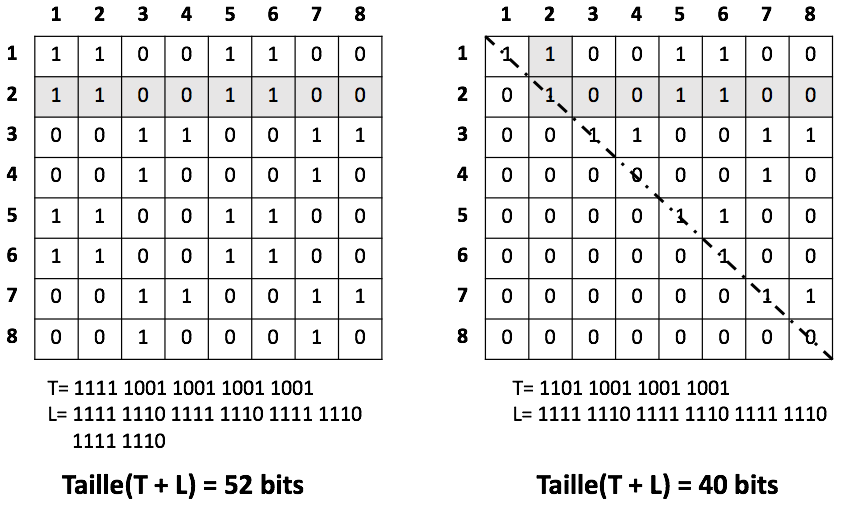
\includegraphics[scale=0.4]{./ressources/image/k2_non.png}
	\caption[Exemple d'arbre $k^2$-tree (k=2) pour un graphe non orienté.]{Exemple d'arbre $k^2$-tree (k=2) pour un graphe non orienté.}
	\label{k2_non}
\end{figure}	


	
	$k^2$-GraCE supporte aussi les graphes dynamiques. Dans le cas de ce type de graphe, il offre la possibilité de calculer une matrice différence à partir de la matrice initiale. Le but de cette fonctionnalité est de maximiser les zones nulles dans la matrice afin de réduire la taille de l'arbre. À \textit{t}=0, on garde la même matrice bidimensionnelle du graphe initial. Pour les instants restants (\textit{t} > 0), nous comparons $M_{pq}$ à l'instant t avec $M_{pq}$ à l'instant \textit{t-1}, si égalité alors la nouvelle matrice contiendra un 0 dans la cellule \textit{pq} à l'instant \textit{t} sinon elle contiendra un 1. La nouvelle matrice d'adjacence contiendra ainsi uniquement les changements qui occurrent entre les instants. La figure \ref{mat_diff} montre une matrice d'adjacence d'un graphe dynamique capturée dans trois instants différents avec sa matrice de différence et la représentation $k^2$-tree dans les deux cas.

\begin{figure}[H]
\centering
	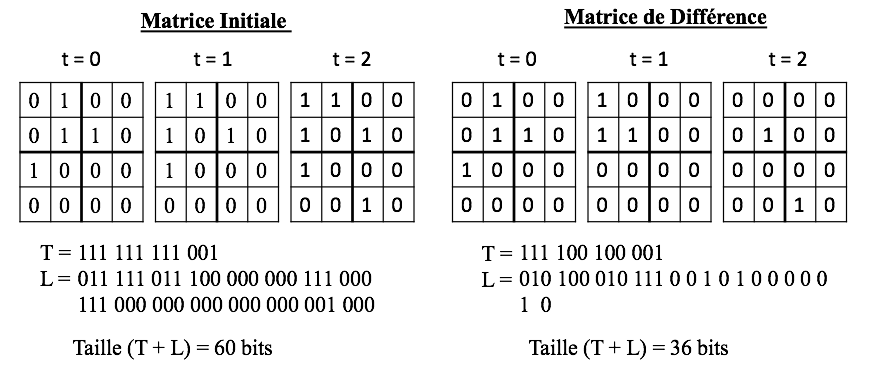
\includegraphics[scale=0.48]{./ressources/image/dynk2diff.png}
	\caption[Exemple d'arbre $k^2$-tree (k=2) pour la matrice de différence]{Exemple d'arbre $k^2$-tree (k=2) pour la matrice de différence.}
	\label{mat_diff}
\end{figure}

L'inconvénient de cette fonctionnalité réside dans le fait qu'une reconstruction de la matrice initiale est nécessaire dans le cas d'interrogation du graphe. Un autre inconvénient de cette technique est qu'elle dégrade les performances dans le cas où les différentes captures ne possèdent pas des arêtes en commun. Dans le cas de disparition de liens par exemple nous obtiendrons des zéros (0) qui vont être remplacés par des uns (1) engendrant ainsi une matrice plus dense. Le gain apporté par cette technique est fortement dépendant des caractéristiques du graphe. 
Nous fournissons ci-après l'algorithme de construction de la matrice de différence :\\

	\begin{algorithm}[H]
					
					\caption{ConstructDiffMatrice}
					\label{alg:diffMat}
					\textbf{Entrée :}
						\begin{itemize}[label=$\bullet$]
							\item M[][][] : la matrice d'adjacence
						\end{itemize}
					\textbf{Sortie :} La matrice de Différence\\							\noindent\rule{\textwidth}{1pt}
						
						
				\begin{algorithmic} [1]
					\STATE MatriceDiff[][][]
					\STATE MatriceDiff[1,:,:] = M[1,:,:]
					\FOR{$i = 2 ... T $} 
						\FOR{$j = 1 ... N $} 
							\FOR{$k = 1 ... N $} 
								\IF {M[i][j][k] = M[i-1][j][k]}
									\STATE MatriceDiff[i][j][k] = 0
								\ELSE
									\STATE MatriceDiff[i][j][k] = 1
								\ENDIF
							\ENDFOR
							
						\ENDFOR
					\ENDFOR
				
					\RETURN MatriceDiff
				\end{algorithmic}
			\end{algorithm}


Nous notons que l'utilisation de ce module dans le processus de construction de l'arbre $k^2$-tree n'est pas obligatoire. Cette phase ne figure pas dans l'algorithme de base. Nous voulons, à travers son intégration dans le moteur \gls{$k^2$-GraCE}, rassembler davantage les nœuds ayant des voisins communs et donc les zones homogènes dans la matrice d'adjacence (zones plaines de 0 ou zones plaines de 1) ou augmenter le nombre de cellules nulles dans la matrice d'adjacence.
		
			\subsubsection{Construction de l'arbre $k^2$-tree}
			
			$k^2$-tree est une représentation compacte de la matrice d'adjacence qui exploite ses propriétés de similarité et de localité. Elle était destinée au départ pour les graphes du web et généralisée par la suite pour différents cas. La représentation est conçue pour compresser les grandes zones nulles de la matrice d'adjacence en les représentant avec un nombre réduit de bits. Plusieurs alternatives existent pour construire l'arbre $k^2$-tree: l'utilisation de la matrice d'adjacence, l'utilisation de la liste d'adjacence ou l'utilisation du graphe directement. Dans tous les cas, nous obtenons une représentation sous forme d'un arbre ayant une hauteur h= $log_k(N)$ où chaque nœud possède $k^2$ fils. 
			  Pour représenter l'arbre de manière concise, deux structures seront utilisées :
			\begin{itemize}
			\item \textbf{T }: Un tableau qui stocke tous les bits du $k^2$-tree sauf ceux du dernier niveau. Les bits de l'arbre $k^2$-tree sont placés après une traversée horizontale de l'arbre. $k^2$-GraCE représente d'abord les $k^2$ valeurs binaires des fils du nœud racine, puis les valeurs du deuxième niveau, ...etc.
			
			\item  \textbf{L} : Un tableau stockant le dernier niveau de l'arbre. Ainsi, il représente la valeur des (ou de certaines) cellules de la matrice d'adjacence du graphe initial.
			\end{itemize}
			
			L'algorithme \ref{alg:k2_tree} résume les différentes étapes de construction de l'arbre $k^2$-tree dans le cas de la construction à partir de la liste d'adjacence. Nous dotons pour cela la liste d'adjacence de \textit{n} curseurs, un par ligne, de sorte que chaque fois que nous devons accéder à $M_{pq}$, nous comparons le curseur actuel de la ligne $p$ à la valeur \textit{q}. S'ils sont égaux, alors on aura $M_{pq} = 1$ et nous devons avancer le curseur vers le nœud suivant de la liste de la ligne \textit{p}. Sinon, nous saurons que $M_{pq} = 0$. 
			
			Nous supposons que la liste d'adjacence $List$, le nombre de fils $k$ ainsi que l'arbre $k^2$-tree $A$ sont des variables globales. Pour construire l'arbre à partir de la racine, elle sera invoquée comme suit :  ConstructK2Tree(N,1,0,0). Après avoir construit l'arbre $A$ sous forme d'un tableau de niveau, nous procèderons à la construction des deux structures selon les deux formules suivantes :
			\begin{itemize}[label=$\bullet$]
			 	\item T = $A_1: A_2:. . . :A_{h-1}$
			 	\item L = $A_h$
			\end{itemize}	

Des versions itératives de l'algorithme peuvent être établies. Cependant, elles dégradent les performances car elles nécessitent soit l'utilisation de structures supplémentaires ou plus d'accès mémoire. Nous avons privilégié la version récursive car elle permet de construire l'arbre $k^2$-tree en un seul parcours de la liste d'adjacence $List$.\\

					\begin{algorithm}[H]
					\label{alg:k2_tree}
					\caption{ConstructK2Tree}
					\textbf{Entrée :}
						\begin{itemize}[label=$\bullet$]
							\item n : la taille de la sous-matrice
							\item l : le niveau de l'arbre
							\item p : l'indice ligne de début de la sous-matrice
							\item q : l'indice colonne de début de la sous-matrice
						\end{itemize}
					\textbf{Sortie :} La valeur du nœud de la sous-matrice\\							\noindent\rule{\textwidth}{1pt}
						
						
				\begin{algorithmic} [1]
					\STATE C = $ \emptyset$
					\FOR{$i = 1 ... k $} 
						\FOR{$i = 1 ... k $} 
							\IF {$l = log_k(N)$} 
								\STATE // Condition selon le type de représentation en entrée 
								\STATE // Matrice d'adjacence : M[p+i,q+j] = 1 
								\STATE // Graphe : $e_{p+i,q+j} \in E$
								\IF { $List$[p+i].courrant() = q+j }
								
									\STATE C = C : 1
									\STATE $List$[p+i].avancer()
								\ELSE
									\STATE C = C : 0
								\ENDIF
							\ELSE
								\STATE  C = C : ConstructK2Tree ( $n/k,l+1,p+i*(n/k), q+j*(n/k)$)
							\ENDIF
						\ENDFOR
					\ENDFOR
					\IF {$C\ est\ un\ vecteur\ nul$} 
						\RETURN 0
					\ENDIF
					\STATE A[l] = A[l] : C
					\RETURN 1
				\end{algorithmic}
			\end{algorithm}
	
	
		Une fois construites, les deux structures (T et L) permettent d'extraire les voisins directs et inverses d'un nœud directement sans décompression. Nous fournissons dans l'annexe \ref{k2_annexe} les détails de ces  algorithmes d'extraction de voisinage.		
			
	

	Un autre type de graphe supporté par notre moteur est le type de graphes dynamiques. Ces graphes sont représentés par un ensemble de graphes statiques chacun capturé à un instant $t_i$. De ce fait, l'algorithme de construction peut être facilement adapté avec chaque nœud dans l'arbre contenant, cette fois-ci, un vecteur de bits chacun faisant référence à un instant $t_i$. Nous fournissons ci-après (algorithme \ref{alg:dynk2_tree}) l'algorithme de construction de l'arbre $k^2$-tree à partir de la matrice d'adjacence tridimensionnelle.\\
	


	
					\begin{algorithm}[H]
					\label{alg:dynk2_tree}
					\caption{DynK2Tree}
					\textbf{Entrée :}
						\begin{itemize}[label=$\bullet$]
							\item n : la taille de la sous-matrice
							\item l : le niveau de l'arbre
							\item p : l'indice ligne de début de la sous-matrice
							\item q : l'indice colonne de début de la sous-matrice
						\end{itemize}
					\textbf{Sortie :} La valeur du nœud de la sous-matrice\\							\noindent\rule{\textwidth}{1pt}
						
						
				\begin{algorithmic} [1]
					\STATE C = $ \emptyset$
					\STATE Creturn  = $ \emptyset$
					\FOR{$i = 1 ... k $} 
						\FOR{$j = 1 ... k $} 
							\IF {$l = log_k(N)$}
								\FOR{$m = 1 ... T $}
									\STATE C[m] = C[m] : M [p+i][q+j][m]
								\ENDFOR
							\ELSE
								\STATE Ctmp =$\emptyset$
								\STATE  Ctmp = DynK2Tree ( $n/k,l+1,p+i*(n/k), q+j*(n/k)$)
								\FOR{$m = 1 ... taille(Ctmp) $}
									\STATE C[m] = C[m] : Ctmp[m]
									\STATE Creturn [m] = Creturn [m] ou Ctmp [m]
								\ENDFOR
							\ENDIF
						\ENDFOR
					\ENDFOR
					\IF {$C\ est\ un\ vecteur\ nul$} 
						\RETURN $0^{|T|}$ // retourner un vecteur nul de taille T.
					\ENDIF
					
					
					
					\FOR{$i = 1 ... k*k $} 
						\FOR{$j = 1 ... T $}
							\IF{ $C[i]$ n'est pas un vecteur nul}
								\STATE A[l] = A[l] : C [i][j]
							\ENDIF
						\ENDFOR
					\ENDFOR
	
					 \RETURN Creturn
					
				\end{algorithmic}
			\end{algorithm}
			
			
	
	
	
	\section{P-GraCE :}
	
	Notre deuxième moteur \gls{P-GraCE} est un moteur de compression par extraction de motifs. Il englobe quatre approches de compression différentes mais qui partagent toutes le même schéma global de compression.  Nous présenterons dans cette partie, en détails, leur principe de fonctionnement et les différents phases qui les constituent.
	
		\subsection{Principe de fonctionnement :}
		
		Les méthodes de compression par extraction de motifs sont des méthodes qui essayent de représenter le graphe de données à travers ses motifs, autrement dit ses sous-graphes portant les informations les plus importantes. 
		
		P-GraCE est un moteur de compression comportant plusieurs méthodes qui peuvent être avec ou sans perte de données. 
		En effet, le modèle produit en sortie (résultat de la compression) est parfois accompagné avec une matrice d'erreur qui sera représentée dans ce cas avec une structure d'arbre $k^2$-tree. Le processus de compression d'un graphe de données par le moteur P-GraCE passe par les étapes suivantes :
		
\begin{enumerate}

\item Lecture et structuration du graphe de données en entrée 

\item Extraction et évaluation des motifs : Durant cette phase, une détection des motifs les plus denses ou les plus fréquents est réalisée. Leur évaluation dans cette phase permet de ne garder que les structures (motifs) susceptibles de donner une meilleur compression.

\item Traitement des motifs: Ce module permet d'encoder ou d'agréger, dans certains cas, les motifs déjà découverts dans le but de minimiser davantage la taille du graphe en sortie. Dans d'autres cas, le module retourne une liste de structures sélectionnées parmi les motifs précédemment identifiés en utilisant des heuristiques dans le but de ne garder que les motifs importants du graphe. %Nous notons que l'utilisation de ce module n'est pas présente dans toutes les méthodes de ce moteur mais dans la plupart 

\item Écriture du graphe compressé sur le fichier de sortie.
\end{enumerate}

La figure \ref{P_grace} permet d'illustrer le principe de fonctionnement globale du moteur \gls{P-GraCE}


\begin{figure}[H]
	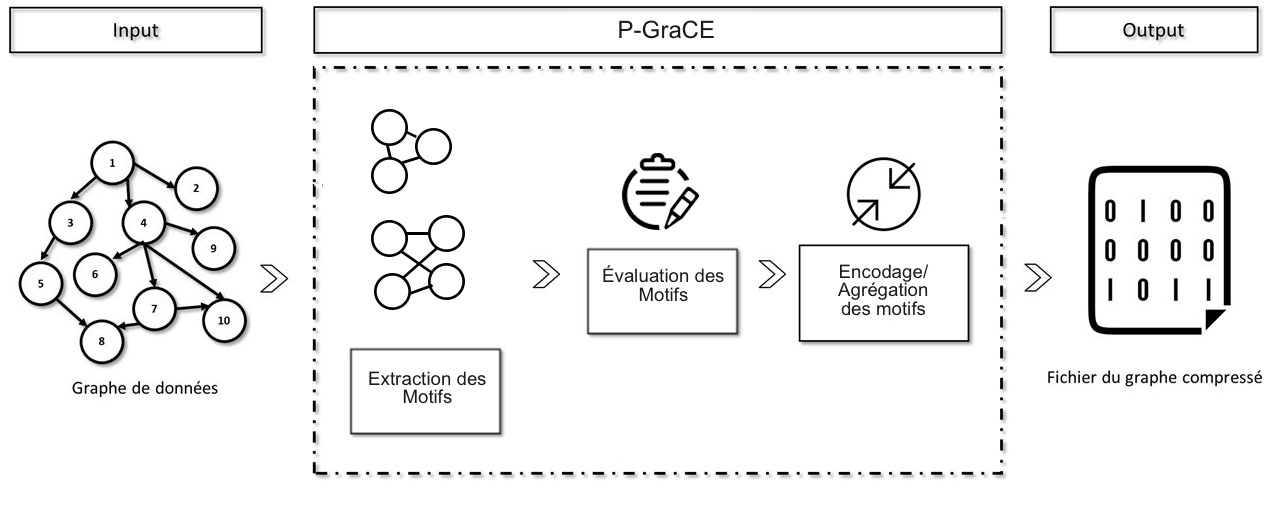
\includegraphics[scale=0.48]{./ressources/image/pgrace.jpg}
	\caption[Vue globale sur le fonctionnement du moteur \gls{P-GraCE}.]{Vue globale sur le fonctionnement du moteur P-GraCE.}
	\label{P_grace}
\end{figure}

Nous présenterons dans ce qui suit les trois phases de chaque approche incluse  dans le moteur P-GraCE. Nous précèderons  cela par expliquer les différents paramètres et notations que nous avons adoptés durant la conception de notre deuxième moteur.
		
		\subsection{Paramètre et notations :}
		
			\begin{table}[H]
		\centering
		\begin{tabular}{|c|L{12cm}|}
		\hline Paramètre & Signification \\ \hline\hline 
		$G$ & Graphe de données \\ \hline
		$V$ & L'ensemble des nœuds de G\\ \hline
		$E$ & L'ensemble des arêtes de G \\ \hline
		$L$ & L'ensemble des étiquettes de G \\ \hline
		$A$ & Matrice d'adjacence du graphe G\\ \hline
		$M$ & Le modèle produit par la compression\\ \hline
		$h$ & Heuristique d'évaluation \\ \hline
		$N$ & Nombre de nœuds dans le graphe \\ \hline
		$k$ & Paramètre déterminant le nombre de fils à considérer dans le beam-search\\ \hline
		
		\end{tabular}
		\caption{Tableau des notations et paramètres du moteur $k^2$-GraCE.}	
		\label{notk2grace}		
	\end{table}
		
		\subsection{Conception modulaire :}
		
		Durant cette section, nous allons présenter les différentes approches qui sont offertes par le moteur P-GracE. Nous commencerons par expliquer les méthodes d'extraction de motifs utilisées dans chacune. Nous enchainerons avec les techniques d'évaluation employées par ces méthodes, pour finir par expliquer comment ces motifs seront traités et utilisés pour compresser le graphe. 	
		
		
		\subsubsection{Extraction des motifs :}

La phase d'extraction de motifs est une phase très importante	 dans le processus de compression. Elle permet de trouver les composantes les plus denses qui représentent en général l'information utile dans un graphe de données. Plusieurs techniques existent pour réaliser cette tâche. Elles diffèrent dans la qualité des sous-structures découvertes selon le domaine d'application et le type de graphe en entrée. Nous présenterons ci-dessous les quatre méthodes offertes par le moteur P-GraCE.
		
\begin{enumerate}

\item \textbf{Beam search:}\\
Le beam search est une méthode de recherche locale gloutonne. C'est une version améliorée de l'algorithme de recherche en largeur \gls{bfs}. Elle permet de n'explorer que les $k$ meilleurs fils dans chaque niveau à travers des heuristiques d'évaluation.

Dans le cas d'extraction de motifs dans un graphe, le beam search commence par considérer que chaque nœud du graphe est un motif. Il utilise pour cela un arbre de recherche où ses nœuds sont des sous-structures. À chaque itération les motifs sont étendus par une arête et un nœud donnant ainsi un ensemble de sous-structures. Par la suite, les $k$ meilleurs sous-structures sont choisies. Les fils restants sont donc élagués. %Le processus continues jusqu'à ce que
Cette alternative sera employée pour le cas des graphes étiquetés. Nous fournissons ci-après l'algorithme du beam search que nous avons utilisé. 


\begin{algorithm}[H]
					\label{alg:beamSearch}
					\caption{Beam-Search}
					\textbf{Entrée :}
						\begin{itemize}[label=$\bullet$]
							\item G : le graphe de donnée
							\item k : le nombre de fils à considérer
							\item limit : limite de la profondeur de l'arbre
						\end{itemize}
					\textbf{Sortie :} retourne la meilleur sous-structure\\							\noindent\rule{\textwidth}{1pt}
						
						
				\begin{algorithmic} [1]
					\STATE C = $\{v\ |\ v$ est un nœud ayant une unique étiquette dans  $G\}$
					\STATE $meilleurStruct$ = la première sous-structure de C
					\REPEAT
					\STATE nouvelC= $\emptyset$
					\FOR{ chaque S dans C} 
						\STATE nouvelStruct = Etendre(S)
						\STATE Evaluer(nouvelStruct)
						\STATE nouvelC = nouvelC $\cup$ \{ les k meilleur sous-structures de nouvelStruct \}
					\ENDFOR
					\STATE limit = limit -1
					\IF {$h$( meilleur sous-structure de C) >= $h$($meilleurStruct$)  }
					
					\STATE $meilleurStruct$  = meilleur sous-structure de C
					\ENDIF
					\STATE C = nouvelC
					\UNTIL{$C = \emptyset $ ou $limit \leq 0$}
					
				\end{algorithmic}
			\end{algorithm}
			
Afin de mieux illustrer le fonctionnement de cet algorithme, nous proposons l'exemple du graphe de la figure \ref{beam}. Nous considérons dans cet exemple qu'un sommet est représenté sur 8 bits, un lien est représenté sur 8 bits et que chaque pointeur est représenté sur 4 bits.


\begin{figure}[H]
	\centering
	
	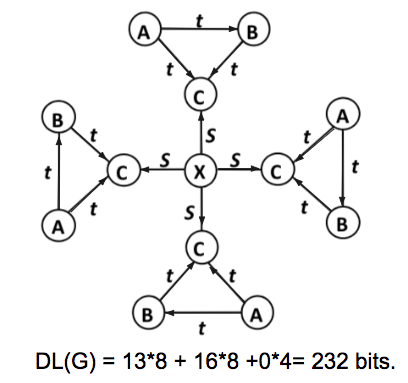
\includegraphics[scale=0.5]{ressources/image/beam_search.png}
	\caption{Exemple de Graphe Étiqueté}
	\label{beam}
 \end{figure}
 
 Au départ chaque nœud est considéré comme une sous-structure, nous obtenons donc quartes sous structures:  A, B, C et X. Par la suite, chacune des sous structures  est étendues par un sommet et une arête tout en estimant le gain obtenu par chaque extension. Nous obtenons donc encore quatre sous structures : A-B, A-C, B-C et X-C. Les trois premières sous-structures donnent le même gain de 24 bits. Tant dis que la quatrième donne une configuration non permise à cause des chevauchements entre ses instances qui possèdent le nœud x  en commun.  La dernière étape donne ainsi le motif A-B-C apportant un gain de 64 bits et qui représente la meilleur sous-structure.  
 
 \begin{figure}[H]
	\centering
	
	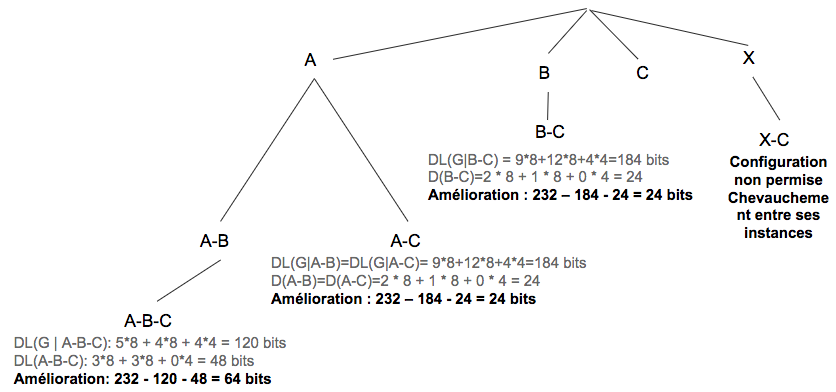
\includegraphics[scale=0.5]{ressources/image/beam_tree.png}
	\caption{Arbre de recherche (k= $ {\infty} $ , limit = $ {\infty} $)}
	\label{beam_tree}
 \end{figure}
 
%Les nœuds du meilleur motif seront agrégés en un seul nœud. La figure \ref{beam_res} donne le résultat finale.  
 
 % \begin{figure}[H]
%	\centering
%	
%	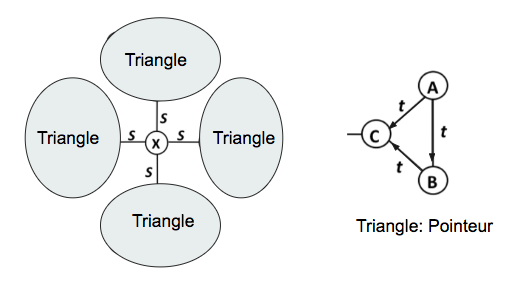
\includegraphics[scale=0.5]{ressources/image/beam_result.png}
%	\caption{Résultat de l'exécution de l'algorithme du beam-search}
%	\label{beam_res}
% \end{figure}


\item \textbf{Méthodes de clustering :}

Plusieurs méthodes de clustering existent dans la littérature. P-GraCE utilise un ensemble de  méthodes de clustering destinées pour compresser un graphe de données en entrée. Nous les détaillons dans ce qui suit. 

\textbf{\textit{SlashBurn}} : Cette technique part de l'observation  que les graphes du monde réel sont facilement décomposables en supprimant leurs nœuds concentrateurs qui sont définies comme les nœuds ayant un degré maximale dans le graphe G.  

%Ce module de P-GraCE permet donc de réordonner les nœuds du graphe de tel sorte à avoir un plus petit nombre de blocs plus denses dans la matrice d'adjacence qui représentent les motifs en sortie.  

À chaque itération le nœud concentrateur est supprimé et le graphe est décomposé en un nœud concentrateur (hub), un
\newacronym{gcc}{CCG}{Composant Connecté Géant}
\gls{gcc} et des rayons restants que nous définissons comme étant le composant connecté non géant connecté aux anciens \gls{gcc}. Le nœud concentrateur obtient ainsi le plus petit identifiant , les nœuds des rayons (spokes) reçoivent les identifiants les plus élevés  dans l’ordre décroissant de la taille du composant connecté auquel ils appartiennent, et le nouveau \gls{gcc} prend les identifiants restants. Le même processus s'applique aux nœuds du nouveau \gls{gcc}, de manière récursive.

Nous illustrons le principe de fonctionnement de cette méthode de clustering sur le graphe de la figure \ref{Img:slashb}. Le nœud concentrateur (8) obtient le plus petit identifiant (1), les nœuds des rayons reçoivent les identifiants les plus élevés (9-16), et le \gls{gcc} prend les identifiants restants (2-8). La prochaine itération considère le nouveau \gls{gcc}. Nous fournissons l'algorithme détaillé en annexe \ref{alg:SlashBurn}.

\begin{figure}[H]
	\centering
	
	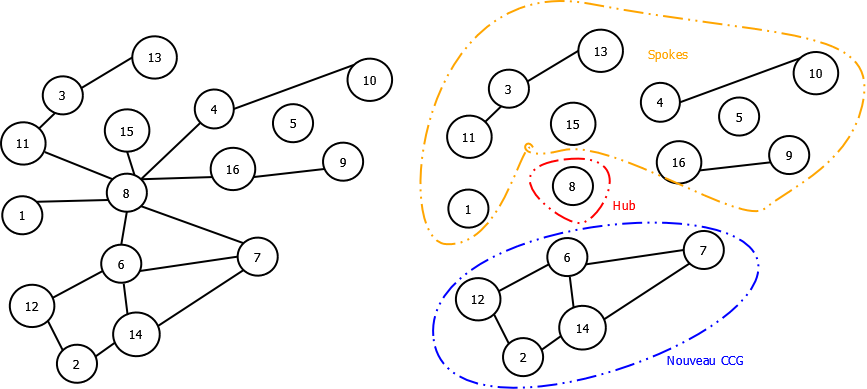
\includegraphics[scale=0.25]{ressources/image/slashburn.png}
	\caption{Exemple d'application de l'algorithme SlashBurn}
	\label{Img:slashb}
 \end{figure}

\textbf{\textit{K-Cores}} : Cette technique se base sur le principe de dégénérescence \footnote{: La dégénérescence d’un graphe G est le plus petit nombre k de
 telle sorte que chaque sous-graphe $S \in G$ contient un sommet de degré au plus k}. Soit G un graphe non orienté, nous notons par $\Delta$(G) le degré maximal des nœuds de G. Un k-core de G est un sous graphe H de taille maximale tel que $\Delta(H) \le k$ avec k entier positif.\\
Pour décomposer le graphe, la méthode passe par quatre étapes. D'abord, le degré k de chaque nœud du graphe est calculé. Ensuite, pour chaque degré k allant du plus grand au plus petit le graphe est décomposé en supprimant tous les nœuds dont le degré est inférieure à k, l'opération s'arrête si la décomposition donne un ensemble non vide et le k est choisit comme $k_{max}$ sinon elle se termine quand $k_{max}$=1. Après la décomposition, chaque composant est identifié comme étant une structure. Enfin, les arêtes entre les structures précédemment identifiées sont supprimées. L'algorithme de la méthode est donné en Annexe (\ref{alg:KCBC})\\


\textbf{\textit{Spectral}} : Cette méthode utilise les résultats d'algèbre linéaire afin de trouver une partition du graphe. L'approche générale consiste à utiliser une méthode de classification standard (généralement k-means) sur  les premiers vecteurs propres (vecteurs de Fiedler) de la matrice Laplaciènne du graphe. La matrice Laplaciènne est définie comme suit : 
\[{M}_{Lap} :=
			\left\{
			\begin{array}{r c l}
			\sum_{k=1}^n poids(i,k)   & si & i=j \\
			-poids(i,j) & sinon
			\end{array}
			\right.
			\]
			\\
Chaque vecteur de Fiedler permet d’obtenir une partition du graphe en
deux parties. Pour partitionner le graphe, nous devons minimiser le coût de coupe de la bissection, cela revient à trouver un vecteur $x \in \{-1,1\}^n $ qui minimise $x^T M_{Lap}x$. Pour cela, nous résolvons le système linéaire $M_{Lap}x = \lambda x$.

L'algorithme prend comme entrée la matrice d'adjacence que nous notons A, une autre matrice diagonal notée D est crée tel que :    
D : \[{d}_{i} := \sum_{(v_i,v_j) \in E_m} e(v_i,v_j)
			\]
			\\
L'algorithme calcule ensuite le deuxième plus petit vecteur propre \textit{y} de la matrice Laplacienne Q = D - A. Ce vecteur propre (vecteur de Fiedler) contient une valeur pour chaque nœud du graphe, à partir de cette valeur le nœud est affecté à l'une des deux partition. Soit r le médian pondéré des valeurs de \textit{y}. Chaque valeur $y_j$ du vecteur propre est comparée à r et le nœud est affecté à une partition selon le résultat de la comparaison.\\
	



\item \textbf{Le MinHash:}

Dans cette alternative, nous allons partitionner le graphe en des motifs denses dont les nœuds sont fortement connectés. Nous utiliserons pour cela une approximation de \textit{la similarité de Jaccard} qui est une métrique permettant de mesurer la similarité entre deux ensembles $S_1$ et $S_2$ (voir formule \ref{eq:Jacc}). 

\begin{equation} \label{eq:Jacc}
SIM(S_1,S_2)=\frac{|S_1 \cap S_2|}{|S_1 \cup S_2|}
\end{equation}


L'objectif de cette méthode est de remplacer les listes d'adjacence des nœuds par des représentations beaucoup plus petites appelées « signatures ». La propriété importante de ces signatures est que leur comparaison permet d'estimer la similarité de Jaccard des listes d'adjacence sans avoir recours à les comparer deux à deux. 

Avant d'expliquer comment il est possible de construire de petites signatures à partir des listes d'adjacence, il est utile de les visualiser en tant que matrice caractéristique. Les colonnes de cette matrice correspondent aux listes d'adjacence et les lignes correspondent aux nœuds. Nous rappelons que la matrice caractéristique est peu susceptible d'être la façon dont les données sont stockées, mais elle est utile pour visualiser les données (voir figure \ref{jacc}). 


Dans un premier temps, k-permutations aléatoires des nœuds devront être choisies. L'utilisation des k-permutations se base sur le fait que :
%% Ajouter demonstration en Annexe ou donner la source 
\begin{equation} \label{eq:prob}
P(\pi_i(S_1) = \pi_j(S_2)) = \frac{|S_1 \cap S_2|}{|S_1 \cup S_2|} = SIM(S_1,S_2)
\end{equation}

 Nous construisons la matrice de signature en considérant chaque ligne dans leur ordre donné. Soit $SIG (i, c)$ l'élément de la matrice de signature pour la $i^{ème}$ fonction de hachage et la colonne c. SIG (i, c) est initialisée à $\infty$ pour tout i et c. Nous traitons une ligne r en procédant comme suit:
\begin{enumerate}
\item nous calculons $h_1 (r), h_2 (r), ..., h_k (r)$.
\item Pour chaque colonne, nous procédons comme suit: 
	\begin{itemize}
		\item  Si c = 0 dans la ligne r, rien à faire.
		\item  Cependant, si c = 1 dans la ligne r, alors pour chaque i = 1,2, ..., k  \\$SIG (i, c)$ = min( $SIG (i, c)$ , $h_i(r)$ ).
	\end{itemize}
\end{enumerate}




Une fois les signatures sont construites, les nœuds ayant les mêmes valeurs seront regroupés. Nous obtiendrons ainsi en sortie la liste des motifs contenant les nœuds ayant un voisinage similaire dans le graphe de données. Nous illustrons le principe de fonctionnement de cette stratégie sur un graphe G dans la figure \ref{jacc}. Le tableau gauche de la figure \ref{jacc} montre une matrice caractéristique des listes d'adjacence des différents nœuds du graphe G ainsi que deux permutations aléatoires $h_1$, $h_2$. Tant dis que le tableau à droite de la même figure montre les étapes de calcul des signatures en utilisant ces deux fonctions. La matrice finale des signatures montre bien que les nœuds 1 et 4 sont les plus similaires ce qui est justifié par leurs listes d'adjacence qui ne diffèrent que dans un seul élément.  

\begin{figure}[H]
\centering
	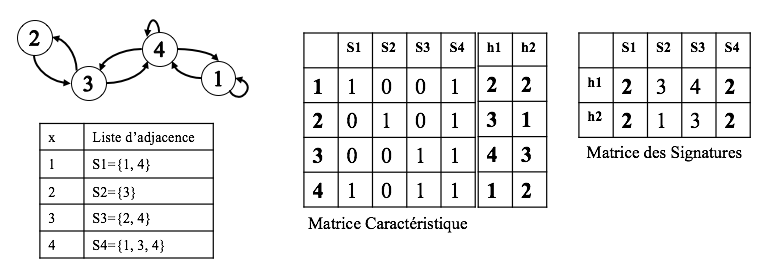
\includegraphics[scale=0.48]{./ressources/image/jacc.png}
	\caption[Exemple de calcul de la matrice des signatures.]{Exemple de calcul de la matrice des signatures.}
	\label{jacc}
\end{figure}

Après l'étape de clustering,  une arborescence est ensuite construite pour chaque ensemble de sommets ayant les même signatures et qui permettra d'extraire les sous-structures (motifs) denses du graphe à travers un parcours de la racine vers les feuilles. 

\item \textbf{Extraction de Motifs de la matrice d'adjacence:}

La dernière méthode d'extraction de motifs offerte par le moteur P-GraCE se base sur les blocs les plus fréquents dans la matrice d'adjacence. Cette méthode est destinée aux graphes ayant une matrice d'adjacence contenant de larges zones nulles. L'ensemble des motifs à découvrir est prédéfinies au départ et consiste en trois types de motifs qui sont paramétrés par la taille du motif :
	\begin{enumerate}[label=(\alph*)]
		\item \textbf{Type 01 :} Ce premier ensemble de motifs consiste en les vecteurs ayant uniquement deux '1', le premier dans le bit de poids fort et un autre dans l'une des position restante, et le vecteur nul. Pour une taille de motif de $2^n$ bits, nous obtenons un ensemble de taille $2^n$.
		
		
		
		\item \textbf{Type 02 :} Le deuxième ensemble de motifs consiste en les vecteurs ayant uniquement un seul '1'. La taille de cet ensemble est de $2^n$ motifs pour des motifs de taille $2^n$ bits.
		\item \textbf{Type 03 :}  Ce dernier ensemble de motifs consiste en l'union des deux ensembles précédents. Dans le cas de cet ensemble, nous obtenons $2^{n+1}$ motifs pour une taille de motifs de $2^n$.
	\end{enumerate}	

Chaque ligne de la matrice d'adjacence est donc divisée en plusieurs blocs ayant la même taille que les motifs. Ces blocs seront comparés avec les motifs selon le type choisi et dans le cas de correspondance ils seront remplacés par l'identifiant du motif (0...n-1) qui est de taille n pour des motifs de taille $2^n$.


	
\end{enumerate}
		
		\subsubsection{Évaluation des motifs :}
		
		 Dans cette deuxième phase, P-GraCE cherche à obtenir la meilleur compression en filtrant les sous-structures et en ne gardant que celles qui offrent un bon \gls{mdl}. 
		 
		 \begin{enumerate}
		 \item Comme nous l'avons déjà précisé P-GraCE utilise le beam-search pour le cas des graphes  étiquetés. Il est fondamentalement guidé par le principe \gls{mdl}. L'évaluation heuristique effectuée suppose que la meilleure sous-structure est celle qui minimise le \gls{mdl} du graphe en entrée lorsqu'il est compressé par cette sous-structure(S). Notons la longueur de description de S par \textit{DL(S)}, la longueur de description du graphe d'entrée G  par \textit{DL(G)} et la longueur de description du graphe après compression par \textit{DL(G|S)}. L'heuristique est alors rien d'autre que le ratio de compression et peut être définie ainsi :
		 
		\begin{center}
		compression = $\frac{DL(G)}{DL(S)+DL(G|S)} $
		\end{center}
		
		\item  Dans le cas de l'utilisation des méthodes de clustering, nous obtenons une liste des structures les plus fréquentes. Pour chaque structure identifiée nous cherchons le motif qui la décrit le mieux en se basant sur un ensemble prédéfini de motifs (étoile, clique, noyau bipartie, semi clique, semi noyau bipartie). Afin de trouver le motif approximatif de la structure, nous utiliserons les formules proposées dans \citep{koutra2015summarizing} (voir section \ref{vog_desc}).
		
		\item Dans le cas de l'utilisation de la technique du MinHashing, nous utilisons le gain apporté par la compression des motifs comme métrique d'évaluation. Nous utilisons pour cela la même formule proposée dans \citep{buehrer2008scalable}. En effet, la qualité de compression d'un motif est calculée en fonction de sa fréquence dans la liste d'adjacence, et de sa taille qui est le nombre de liens qu'il contient (Formule \ref{eqcompperf}).
				%%% Formule
				\begin{equation}
				Compression(P)=(P.frequence-1)(P.taille-1)-1
				\label{eqcompperf}
				\end{equation}
				
		\item Dans le cas de l'extraction de motifs à partir de la matrice d'adjacence aucune évaluation n'est nécessaire car tout les motifs offrent le même gain d'espace mémoire.
		 
		
		 \end{enumerate}
		 
		   
		\subsubsection{Traitement des motifs :}
		
		Nous proposons pour traiter les motifs dans le moteur P-GraCE plusieurs alternatives, cela dépend de la méthode utilisé.
		
La première consiste à faire une agrégation des nœuds du meilleur motif. Les trois étapes seront donc répétées jusqu'à ce que la taille du graphe en sortie ne peut plus être optimisée. Elle est appliquée dans le cas de l'approche beam-search.

 La deuxième alternative consiste à considérer que  la liste des sous-structures de l'étape 2 représentent le compressé du graphe de données. Nous effectuons une sélection à partir de l'ensemble des structures initiales pour obtenir un modèle (ensemble de structures) avec un MDL optimal. Cette option sera employée dans  l'approche basée sur les méthodes de clustering . La sélection se fait à travers plusieurs algorithmes. Nous présentons ci dessous les méthodes que nous allons utiliser durant cette phase:
\begin{itemize}
\item Top10 : Cette méthode commence par ordonner les sous structures selon le gain de codage local apporté par chacune d'elles. Le gain de codage local est définit par L(g,$\emptyset$) - L(g,$\omega$) où L(g,$\emptyset$) représente le codage de g (g est le sous graphe contenant la structure) en tant qu'erreur (un modèle vide) et L(g,$\omega$) est le cout de codage de g avec la structure $\omega$. Elle sélectionne ensuite les k meilleurs structures ayant un gain local élevé. \newacronym{gnf}{GNF}{Greedy'nForget}
\item \gls{gnf} : Au lieu de prendre en compte toutes les combinaisons possibles des structures, l'heuristique 
\gls{gnf}
 considère les structures selon un ordre décroissant de leur gain d'encodage local. Elle parcourt structure par structure et inclut dans le modèle celle qui réduit le MDL. L'algorithme de \gls{gnf} est présenté dans ce qui suit (\ref{alg:GNF})   

\end{itemize}

\begin{algorithm}[H]
\label{alg:GNF}
	\caption{Geedy'nForget}
		\textbf{Entrée :}
		\begin{itemize}[label=$\bullet$]
			\item $\mathcal{C}$ : Listes des structures évaluées.
							
							
			\end{itemize}
	\textbf{Sortie :} ensemble des structures sélectionnées $\mathcal{M}$\\							\noindent\rule{\textwidth}{1pt}
								
	\begin{algorithmic} [1]
	 \STATE MDL-optimal = MDL(G,$\emptyset$)
\STATE Ordonner($\mathcal{C}$,"descendant") 
	\FOR{ $s \in \mathcal{C}$ }
	\STATE $\mathcal{M} = \mathcal{M} \cup {s}$ 
		\IF{ MDL(G,$\mathcal{M}$) <  MDL-optimal}
			\STATE MDL-optimal = MDL(G,$\mathcal{M}$)
		\ELSE 
			\STATE $\mathcal{M}$ = $\mathcal{M} \setminus {s}$  \COMMENT{Enlever la structure de l'ensemble}
		\ENDIF
	\ENDFOR   
	\end{algorithmic}
		\end{algorithm}

\begin{itemize}
\item STEP : Cette méthode parcourt de manière itérative toutes les structures évaluées précédemment dans un ordre quelconque et choisit la structure qui réduit le plus le MDL du modèle courant pour l'ajouter au modèle jusqu'à ce qu'aucune structure n'améliore le cout. Nous présentons l'algorithme détaillé ci-dessous :


\end{itemize}

\begin{algorithm}[H]
\label{alg:STEP}
	\caption{STEP}
		\textbf{Entrée :}
		\begin{itemize}[label=$\bullet$]
			\item $\mathcal{C}$ : Listes des structure évaluées.
							
							
			\end{itemize}
	\textbf{Sortie :} ensemble de structures sélectionnées $\mathcal{M}$\\							\noindent\rule{\textwidth}{1pt}
								
	\begin{algorithmic} [1]
	\STATE Best-Structure = -1
	 \STATE MDL-optimal = MDL(G,$\emptyset$)
	\WHILE{$\mathcal{C}$ != $\emptyset$}
	\FOR{ $s \in \mathcal{C}$ }
	\STATE $\mathcal{M} = \mathcal{M} \cup {s}$ 
		\IF{ MDL(G,$\mathcal{M}$) <  MDL-optimal}
			\STATE MDL-optimal = MDL(G,$\mathcal{M}$)
			\STATE Best-structure = s
		\ENDIF
		\STATE $\mathcal{M}$ = $\mathcal{M} \setminus {s}$  //Enlever la structure de l'ensemble
	\ENDFOR
	\IF{Best-Structure != -1}
	   \STATE $\mathcal{M} = \mathcal{M} \cup {Best-structure}$ 
	   \STATE Best-Structure = -1
	   \ELSE 
	   \STATE STOP
	  \ENDIF
		\STATE $\mathcal{C}$ = $\mathcal{C} \setminus {s}$
	\ENDWHILE
	\end{algorithmic}
		\end{algorithm}
		
\begin{itemize}
\item Pour la méthode du minhashing, nous offrons  la possibilité d'utiliser le codage proposé dans \citep{liu2018reducing}. Il représente cette liste de motifs de manière concise tout en permettant les requêtes d'extraction de voisinage. %Dans certaines méthodes une matrice d'erreur est conservée avec la liste des structures pour une compression sans perte.
\end{itemize}

		
		
		
	\section{Notre méthode: Dynamic Dense Subgraph Mining (DDSM)}
		
Comme on vient de voir dans les chapitres précédents, de nombreux phénomènes dans des contextes très variés peuvent être représenter par des graphes. Citons en particuliers les réseaux sociaux qui nous attirent vu leur importance et leur fort impact sur la vie réel. En effet, trois quarts des personnes connectées à internet utilisent les réseaux sociaux. Ils rassemblent aujourd'hui 3,169 milliards d'utilisateurs actifs, voir 40\% de la population sur terre, avec 11 personnes s'inscrivant chaque seconde sur Facebook, Twitter et autres
\footnote{https://bfmbusiness.bfmtv.com/hightech/la-moitie-de-la-population-mondiale-est-connectee-a-internet-1361933.html}. De ce fait, deux constats s'impose: le premier est l'incapacité des graphes statiques à décrire certaines situations de la vie réelle et leur évolution dans le temps, le deuxième est la montée en flèche de la quantité et l'hétérogénéité des informations modélisées par ces réseaux et qui rendent presque impossible tout traitement. D'où le besoin croissant de méthodes de compression de graphes dynamiques. 

Nous nous sommes aussi intéressées dans ce travail à un autre enjeu important qui est la recherche de motifs et particulièrement les clique et les noyaux bipartie qui sont fréquents dans les réseaux faisant abstraction à des situations réelles importantes dans le processus de prise de décision. Nous citons par exemple, les attaquants de réseaux de botnet formant un noyau bipartie avec leurs victimes pendant la durée d'une attaque, les membres de la famille se liant comme une clique au cours d'une période difficile, ou les collaborations de recherche s'étant créées et qui disparaissent au cours des années.

%Quoiqu'il existe de nombreuses techniques de compression efficaces adaptées au contexte statique, rares sont ceux qui proposent une contrepartie dynamique, ce qui nous amène à s'intéresser particulièrement à ce type de graphes toujours en cours d'évolution. 

Nous allons dans cette partie proposer une nouvelle méthode \gls{ddsm} basée sur deux approches existantes que nous avons étudié dans notre état de l'art. Notre but principal est de développer une technique de compression compétitive pour les graphes des réseaux sociaux dans un contexte dynamique en se basant sur l'extraction de motifs. Pour accomplir ce travail nous nous sommes appuyés sur ces deux méthodes :
\begin{itemize}
\item Exploiter la structure de données compressée proposée dans \gls{dsm} \citep{hernandez2014compressed} qui permet de représenter les sous-graphes denses comme les cliques, les quasi-cliques, noyaux bipartis. Nous avons opté pour cette structure car en l'appliquant sur les réseaux sociaux, elle donne de bons résultats en matière d'espace et de temps de requêtes.  
\item Adopter les signatures temporelles utilisées dans TimeCrunch \citep{shah2015timecrunch} pour décrire le comportement des sous-graphes dans le temps. Nous avons utilisé ces signatures car elles englobent tous les types de comportements temporels d'un motif dans un graphe dynamique.
\end{itemize}	
%Nous allons dans cette partie présenter notre méthode théoriquement : principe général, structure utilisée et un pseudo code.	
		
		\subsubsection{Formulation du problème}
		Dans cette section, nous allons définir le problème de base auquel notre méthode convient tout en définissant le cadre dans lequel elle peut être appliquée. 
		
		Nous considérons les graphes orientés dynamiques $\displaystyle{G=\bigcup_{t_{i}}G_{t_{i}}(V,E_{t_{i}})}\ \ 1 \preceq i \preceq t$ où $G_{t_{i}}$ = G a l'instant $t_{i}$ et un ensemble de signatures temporelles. En d'autre termes, nous considérons des captures du graphe à des instants différents $t_{i}$ et un ensemble de descripteurs de comportement temporel des sous-graphes des différents $G_{t_{i}}$. Le problème peut ainsi être formulé:
		
			\textit{\textbf{Problème:}
		Trouver, à partir d'un graphe dynamique G et un lexique de signatures temporelles, la plus petite description du graphe initial en termes de ses sous structures les plus denses et leur comportement temporel, en offrant la possibilité de manipuler le graphe, d'extraire les voisins directs d'un nœud à un instant donné et d'extraire les sous-graphes au besoin. }

		\subsubsection{Principe général}
			Notre méthode s'intitule DDSM pour \textit{Dynamic Dense Substructure Mining}. Elle représente une généralisation du travail de Hernandez et Navarro \citep{hernandez2014compressed} pour le cas des graphes dynamiques qui sont de nos jours omniprésents.
			
			%Pour mieux expliquer notre méthode nous allons tout d'abord commencer par décrire les structures que nous allons utiliser. Nous enchainons par la suite  avec le pseudo algorithme détaillant les étapes essentielles de notre méthode et nous conclurons en expliquant comment les algorithmes proposés dans \citep{hernandez2014compressed} de manipulation des graphes peuvent être généralisés dans notre cas.
			%\subsection{Description conceptuelle}
			
			La codification du graphe en sortie doit respecter les contraintes du problème tout en réduisant un maximum d'espace mémoire. Pour cela, Nous proposons d'étendre la codification proposée dans \citep{hernandez2014compressed} pour le cas des graphes dynamiques en rajoutant une information temporelle. 
			
			Une fois les sous-structures identifiées, Hernandez et al. \citep{hernandez2014compressed} proposent de représenter chacune d'elles avec trois composantes: la première contenant les sommets ayant uniquement des arêtes sortantes, la deuxième contenant les sommets ayant des arêtes entrantes et sortantes et la troisième contenant les sommets ayant uniquement des arêtes entrantes. Pour pouvoir identifier les différentes composantes, ils associent un vecteur binaire à cette représentation marquant par un 1 le début de chacune des trois composantes (voir figure \ref{SDM}).
			
			Notre première contribution consiste en l'extension de cette structure. En effet, nous suggérons de représenter chaque sous structure avec non pas trois composantes mais quarte composantes. Les trois premières étant les même que dans \citep{hernandez2014compressed}, la quatrième représente l'information temporelle. Cette dernière peut avoir cinq formats (voir section \ref{par:TimeCrunch}) dont nous résumons la représentation proposée pour chacune dans le tableau \ref{tab:signtmp}.
			
			\begin{table}[h]
			\label{tab:signtmp}
			\begin{center}
			\begin{tabular}{|r|l|}
			\hline Signature temporelle & Représentation	
			\\\hline constante & 0	
			
			\\\hline OneShot & 1 $t_{1}$	
			
			\\\hline ranged & 2	$t_{1}\ t_{2}$	
			
			\\\hline periodic & 3  $T$	
			
			\\\hline flikering & 4 $t_{1}\ t_{2}\ ...\ t_{n}$	
			
			\\\hline			
			\end{tabular}
			\end{center}
			
			 \caption{\small {Les types de signatures temporelles et leurs représentations, $t_{i}$	 représentent les timestamps et T représente la période.}}
			\end{table}
			
			Nous représentons G donc comme un ensemble de sous-graphes temporels denses. Cependant, pour obtenir une compression sans perte, nous devons aussi garder l'erreur modélisant l'ensemble d'arêtes restantes dans chaque $G_{t_{i}}$. Nous proposons pour cela d'utiliser une des structures dynamiques des k2-trees qui nous permettra d'interroger le graphe de manière simple et efficace.
			
			%\subsection{Notre méthode : DDSM}
			 Nous visons à travers la méthode que nous proposons d'exprimer le graphe en entrée avec ses sous-structures les plus denses et leur comportement temporel réduisant ainsi sa taille et offrant la possibilité d'effectuer les traitements dans un temps meilleur. Nous avons structuré notre algorithme sous forme de trois (03) étapes essentielles, chacune servant d'entrée pour l'étape suivante.
			 
			 En premier lieu, nous appliquons la découverte des sous-graphes les plus denses. Pour effectuer cela de manière efficace, nous suggérons d'utiliser l'approche proposée dans \citep{hernandez2014compressed} parallèlement sur chaque capture $G_{t_{i}}$ de G. Nous allons donc considérer les listes d'adjacences pour chaque $G_{t_{i}}$ où des fonctions de hachage sont calculées pour chaque sommet. Une arborescence est ensuite construite pour chaque ensemble de sommets ayant les même valeurs de hachages et qui permettra d'extraire les sous-structures denses du graphe à travers un parcours de la racine vers les feuilles. Dans une deuxième phase, nous effectuons une comparaison entre les sous-structures découvertes dans des timestamps différents afin de lui associer la signature appropriée. Durant cette étape, nous tolérons un certains seuil d'erreur qui sera inclus dans la représentation de l'erreur. Une dernière phase consiste en la codification du graphe en utilisant le codage proposé dans la section précédente pour chaque sous-structure de la phase (02). Nous concaténons par la suite ces représentations pour obtenir une seule représentation concise du graphe initial en termes de ses structures les plus denses. 
			L'algorithme \ref{alg:DDSM} résume les trois principales étapes de notre méthode.
			\begin{algorithm}
					\label{alg:DDSM}
					\caption{DDSM}
					\label{Pseudo Algorithme de la méthode proposée (DDSM)}
				\begin{algorithmic} [1]
					\STATE \textbf{Génération des sous structures candidates: }Génération de sous-graphes, principalement les sous-graphes bipartis et les cliques.
					
					\STATE  \textbf{Étiquetage de sous-structures: }Associer chaque sous-structure à une signature temporelle décrivant son comportement.
					
					\STATE \textbf{Codification du graphe compressé: }Codifier les sous-structures étiquetées de l'étape (02) en utilisant les structures de la section précédente.
				\end{algorithmic}
			\end{algorithm}
			
			Pour les algorithmes de parcours et d'extraction de voisins, tous les algorithmes proposés dans \citep{hernandez2014compressed} peuvent être généralisés sur notre structure. En effet, le seul changement consiste en la  prise en compte de l'information temporelle dans l'incrémentation des indices de parcours. De ce fait, nous pensons que notre méthode peut offrir un très bon compromis entre l'espace mémoire et le temps d'accès des traitements dans le cas des graphes dynamiques. 
			
		%\subsubsection{Conclusion}
	%Dans ce chapitre, nous avons abordé le problème de compression des graphes dynamiques par extraction de motifs. Nous avons formalisé le problème de compression d'un graphe dynamique en se basant sur les sous-graphes denses temporelles qui le composent. Pour faire face à ce problème nous avons présenté une nouvelle méthode hybride intitulée DDSM, elle combine deux méthodes de la littérature que nous avons jugé efficaces. Notre prochain but est de tester cette méthode en la comparant avec les méthodes existantes.   

	
	
	\section{Conclusion}

Dans ce chapitre, nous avons expliqué la partie conceptuelle de nos deux moteurs: $k^2$-GraCE et P-GraCE, qui  représentent les deux classes qui font l'objet de notre recherche. Nous avons présenté leur différents modules et fonctionnalités tout en clarifiant leurs paramètres ainsi que leur principe de fonctionnement.

	Dans le chapitres suivant, nous présenterons les choix d'implémentation que nous avons effectués. Nous décrirons l'environnement de développement ainsi que l'architecture globale de notre projet. 
	
	
	

	

\chapter{Implémentation}
	\section{Introduction}
	
	Notre projet s'intègre dans un projet de recherche scientifique. De ce fait, une implémentation efficace et optimisée de notre conception est nécessaire. Nous commencerons ce chapitre par présenter l'architecture existante et comment nous l'avons étendue avec nos deux moteurs tout en détaillant les différentes couches de cette architecture. Nous conclurons par présenter l'environnement de développement.
	
	
	\section{Architecture globale}
	
	L'architecture existante est une architecture en pipeline de 3-tiers. Nous  adopterons cette même architecture. Elle se compose de trois couches logicielles que nous avons enrichies avec nos deux moteurs. Nous les présenterons ci-dessous:
	
	\begin{enumerate}
	\item \textbf{La couche données ou persistance :} cette couche est responsable de la gestion des données en entrée et les fonctions d'accès et de stockage. Les données en entrée ainsi que les résultats de compression sont sous forme de fichiers.
	
	\item \textbf{La couche traitement :} c'est le noyau des moteurs de compression de notre projet. Elle inclue tout les algorithmes de compression et de manipulation des graphes. 
	
	\item \textbf{La couche présentation :}  Deux types de résultats (fichiers) sont produits : le premier est le graphe compressé, le deuxième représente le fichier log des performances. 
	\end{enumerate}
		
	
\begin{figure}[H]
	\centering
	
	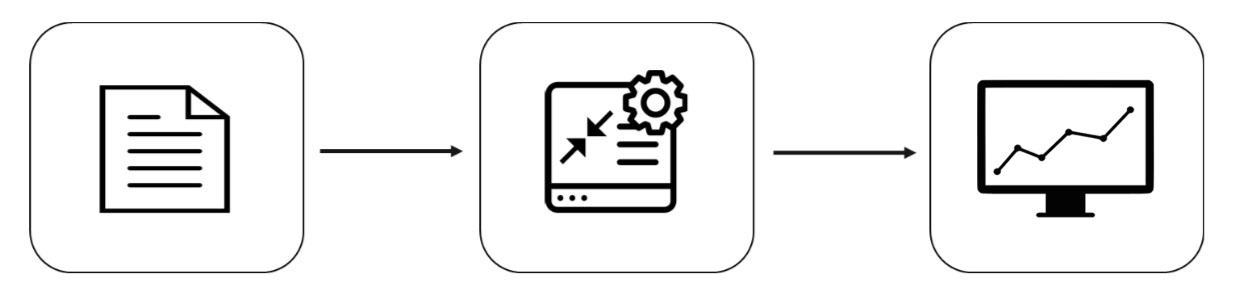
\includegraphics[scale=0.35]{ressources/image/ArchGlob.jpg}
	\caption{Architecture du globale}
	\label{Img:archglob}
 \end{figure}
	
%	Dans le but de faciliter l'exploitation et l'utilisation de notre solution, nous proposons une application web qui permettra  d'accéder aux différentes fonctionnalités offertes. Cette proposition se base sur le fait que les performances des machines ordinaires s'avèrent limiter pour l'exécution des algorithmes de compression dans le cas des grands graphes. L'utilisation d'un serveur web performant nous semble la solution la plus adéquate. La figure \ref{Img:archglob2} montre l'architecture globale de la solution.   	
	
%\begin{figure}[H]
%	\centering
%	
%	
\includegraphics[scale=0.35]{ressources/image/ArchGlob2.jpg}
%	\caption{Architecture globale de la solution web}
%	\label{Img:archglob2}
% \end{figure}
 
% Dans ce qui suit, nous détaillerons uniquement les couches de l'architecture du backend ainsi que les bibliothèques qui les constituent. Les détails des autres couches de l'architecture globale ne seront pas présenter car elles n'influence en aucun cas sur les résultats de compression. Elle permettent uniquement d'offrir une interface ergonomique et une exécution distante tirant profit de la force de calcul du serveur utilisé.
	
	\section{Données}
	Les données manipulées par les moteurs de compression sont tous sous format de fichiers texte. La structure de ces fichiers diffère selon le type du graphe en entrée. Comme nous l'avons déjà implicitement mentionné, l'implémentation proposée prend en charge les types de graphes suivants : graphe dynamique orienté, graphe statique (orienté et non orienté) et finalement graphe étiqueté. Nous présenterons dans ce qui suit leurs structures:
	
	\begin{itemize}[label=$\bullet$]
	\item \textbf{Graphe statique:}
	
	\begin{figure}[H]
	\centering
	
	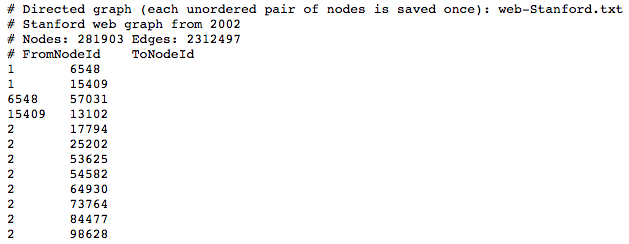
\includegraphics[scale=0.65]{ressources/image/statiqugr.png}
	\caption{Structure d'un fichier de graphe statique}
	\label{Img:statiqugr}
 \end{figure}
	
	Le fichier représentant un graphe statique est composé de plusieurs lignes chacune faisant référence à un des liens du graphe de données. Elles incluent l'identifiant de la source suivi de  l'identifiant de la destination. Les lignes dont le premier caractère est un "\#" sont ignorées.
	\item \textbf{Graphe dynamique: } 
	
	\begin{figure}[H]
	
	
	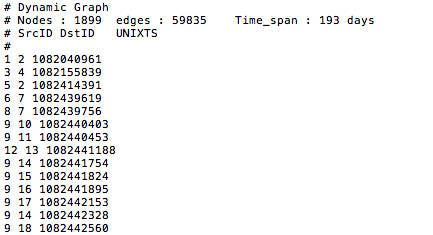
\includegraphics[scale=0.7]{ressources/image/dynamiqgr.png}
	\caption{Structure d'un fichier de graphe dynamique}
	\label{Img:dynamiqgr}
 \end{figure}
Les liens dans un graphe dynamique sont représentés par trois composantes (u,v,t)	signifiant qu'un lien entre les nœuds u et v appartient à la capture de l'instant t. Chaque lien représente une ligne dans le fichier de données.
	
	\item \textbf{Graphe étiqueté:} 
	\begin{figure}[H]
	
	
	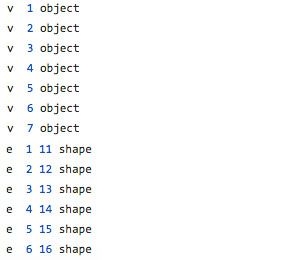
\includegraphics[scale=0.6]{ressources/image/etiquegr.png}
	\caption{Structure d'un fichier de graphe étiqueté}
	\label{Img:etiqGr}
 \end{figure}

Le fichier de données d'un graphe étiqueté est composé de deux types de lignes: les lignes commençant avec un "$v$" représentent les identifiants des sommets suivis de leurs étiquettes et les lignes commençant avec un "$e$" représentent les sommets source et destination des liens suivis de leurs étiquettes.
	
	\end{itemize}
	
	
	
	\section{Traitement}

Dans cette section, nous détaillerons les principales structures utilisées pour représenter les graphes en mémoire ainsi que les fonctions et méthodes décrivant les interfaces de nos deux moteurs  de compression. 
\subsection{Les structures utilisées }
Nous nous intéressons dans notre projet à trouver un bon compromis entre les performances de la compression (taux de compression et le nombre de bits par nœud) et le temps d'exécution. Pour cela nous avons essayé de choisir des implémentations de structures de données qui répondent à cette contrainte.

\begin{enumerate}[label=(\alph*)]
\item \textbf{TNGraph :}
Cette structure est l'une des structures les plus performantes offertes par la bibliothèque \newacronym{snap}{SNAP}{Stanford Network Analysis Package}	 \gls{snap} (voir section \ref{snaplib}). Elle représente un graphe orienté et est implémenté à l'aide de fonctions de hachage offrant ainsi un temps d'accès très rapide. Elle offre aussi une panoplie d'opérations facilitant la manipulation du graphe de données.

\item\textbf{TUNGraph :}
Cette structure est aussi une des structures de la bibliothèque \gls{snap}. Elle représente un graphe non orienté et offre les mêmes avantages que la structure précédente. 

\item\textbf{std::vector<Boost::dynamicbitset<> > :}
 Nous avons adopté cette structure pour représenter la matrice d'adjacence en mémoire. Les lignes de la matrice d'adjacence sont représentées par un vecteur de bits de la bibliothèque Boost donnant un accès rapide comparé aux implémentations disponibles  \citep{pieterse2010performance}. Les tableaux de lignes seront stockés dans un tableau de la bibliothèque standard du langage c++ permettant d'exploiter la localité du cache. %vu que ses éléments sont stockés de façon contigüe en mémoire.
 
\item\textbf{std::vector<std::pair<std::vector<unsigned int>,unsigned int> >:}
Cette structure représente la liste d'adjacence d'un graphe. Comme nous l'avons déjà expliqué nous dotons chacune des listes par un pointeur indiquant la position du dernier élément visité. Les paires ( listes, pointeurs ) seront stockées dans un tableau indexé par les identifiants des nœuds du graphe ( 0...N ).

\item\textbf{LabeledGraph :} Pour les graphes étiquetés, nous proposons d'utiliser notre propre structure intitulée << \textit{LabeledGraph} >>.

\item \textbf{std::map<unsigned int,TNGraph> :}
La dernière structure modélise les graphes dynamiques orientés qui sont représentés par les paires ($t_i$ , $G_i$) où $G_i$ représente une capture du graphe de données à l'instant $t_i$.


\end{enumerate}



\subsection{Les méthodes et fonctions }
	Nous présenterons ci-dessous les principales fonctions et méthodes décrivant le schéma global de fonctionnement de nos deux moteurs.
	
	\begin{enumerate}[label=(\alph*)]
		\item \textbf{LoadGraph :} Cette fonction permet de charger le graphe de données en mémoire à partir d'un fichier texte. Elle prend en paramètres le fichier de données ainsi que le type de graphe dans le cas du moteur P-GraCE. Dans le cas du moteur $k^2$-GraCE, elle prend en paramètres le fichier de données, le type de graphe, le type représentation à utiliser pour compresser le graphe ainsi que le choix d'activer ou non le module de pré-traitement.
		
		\item \textbf{CompressK2 :} Cette fonction consiste en le processus de compression du graphe en utilisant les arbres $k^2$-trees. Elle reçoit en entrée le graphe de données et son type et donne en sortie les deux listes T et L représentant l'arbre $k^2$-trees.
		
		\item \textbf{CompressPattern :} Cette fonction permet de compresser le graphe de données en utilisant ses sous-structures les plus importantes. Elle prend en paramètres le graphe de données ainsi que le choix de l'approche de compression à utiliser et ses paramètres.
		
		\item \textbf{SaveCompressed :}  Cette fonction effectue la sauvegarde du résultat de compression dans un fichier texte.
		
	\end{enumerate}	
	
	Le schéma de la figure \ref{Img:functMethod} montre le schéma globale de fonctionnement des deux moteurs:  
	
	\begin{figure}[H]
	
	
	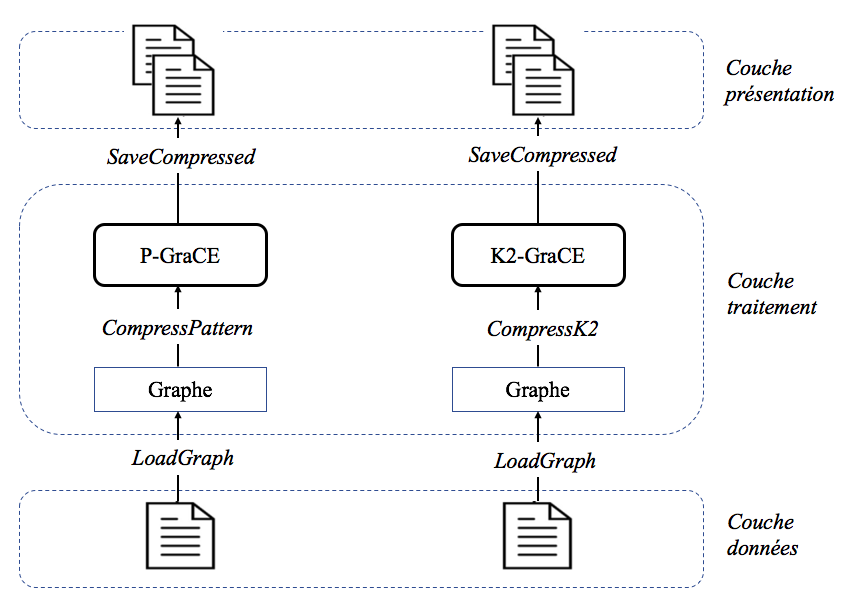
\includegraphics[scale=0.5]{ressources/image/funct.png}
	\centering
	\caption{Schéma globale du fonctionnement des deux moteurs}
	\label{Img:functMethod}
 \end{figure}
	
	
	\section{Présentation}
	
	La couche présentation est responsable de donner accès à toutes les fonctionnalités offertes par notre solution, entre autre le choix des paramètres pour différentes méthodes, ainsi que de visualiser les résultats. En plus du fichier de sortie, elle fournit les différentes mesures de performances. Elle offre ainsi aux chercheurs la possibilité de comparer les performances de différentes méthodes sur un même graphe. 
	
	\section{Environnement de développement}
		
		Le choix des outils de développement dans tout projet informatique est très important vu leur fort impact sur les performances du produit final. Comme notre solution fait partie d'un projet de recherche, il faut aussi prendre en compte la flexibilité et la capacité de la solution à s'interfacer avec d'autre outils dans des systèmes qui peuvent être hétérogènes. 
		
		\subsection{Langage de Programmation}
		Nous avons adopté le langage de programmation avec lequel la    première version de notre solution a été développée: le C++. En effet, il représente un langage très performant pour les calculs lourds. Il permet d'avoir des exécutions très rapides, ce qui en fait un langage de choix pour les applications critiques qui ont besoin de performances. Il permet aussi d'avoir un code portable : un même code source peut être facilement transformé en exécutable sous Windows, Mac OS ou Linux. Un autre aspect du langage c++ est sa richesse de bibliothèques optimisées pour le traitement et le stockage des grands graphes en mémoire. 
		
		Nous avons choisi Visual Studio 2015 comme environnement de développement (IDE). Notre choix a été influencé par le fait que Visual Studio s'ouvre à toutes les tendances du moment et permet facilement de travailler en équipe sur le même projet.
		
		\newacronym{ide}{IDE}{Integrated Developement Environement} 
		\subsection{Bibliothèque Snap}
		\label{snaplib}
			
		Afin de faciliter la manipulation des graphes et d'améliorer les performances de notre solution, nous avons offert la possibilité d'exécuter les différents algorithmes de compression en utilisant une des plus performantes bibliothèques de manipulation de graphes en c++ : SNAP.
		\gls{snap} est une bibliothèque d'analyse et d'exploration de graphes à usage général qui s'adapte facilement à des graphes massifs. Elle présente aussi l'avantage d'être  efficace et facilement extensible. 
		
		\subsection{Bibliothèque Boost}
		

Boost est un ensemble de bibliothèques pour le langage de programmation C ++ qui prend en charge des tâches et des structures telles que l'algèbre linéaire, la génération de nombres pseudo-aléatoires, le multithreading, les expressions régulières et les tests unitaires. Elle contient plus de quatre vingt bibliothèques individuelles.

Nous l'avons utilisée dans notre projet pour l'implémentation des arbres $k^2$-trees. En effet, elle contient une implémentation des tableaux de bits en c++ qui donne un temps d'exécution optimal comparé aux autres implémentations existantes \citep{pieterse2010performance}.  


	\section{Conclusion}
	
Durant ce chapitre, nous avons présenté notre implémentation où nous avons essayé d'utiliser différentes bibliothèques permettant d'avoir les meilleurs performances. L'indépendance des différentes couches de l'architecture existante nous a facilité la tache d'implémentation. Nous avons ainsi essayé de respecter cette indépendance afin de faciliter tout autre contribution future dans le projet. 

Nous évaluerons dans le chapitre suivant les différentes méthodes de nos deux moteurs en vue de l'obtention d'une étude comparative plus objective et plus claire de leur performance.
	
	\chapter{Test}
	\section{Introduction}
	
Dans ce chapitre, nous exposerons les différents résultats des mesures de performances obtenus par nos deux moteurs $k^2$-GraCe et P-GraCe en utilisant plusieurs datasets dans différentes configurations. Nous commencerons par présenter l'environnement de test et les conditions d'expérimentation ainsi que les graphes utilisés. Nous allons par la suite présenter les résultats obtenus pour chaque méthode séparément et comparer par la suite entre les deux moteurs k2-GraCE et P-GraCE. 


	
	
	\section{Environnement de Test}
	L'environnement de test compte parmi les éléments sur lesquels repose l'optimisation de tout système. C'est un environnement permettant de tester les différentes configurations et modules. Nous présenterons dans cette partie les caractéristiques matérielles et logicielles de l'environnement de test utilisé durant nos expériences. 

	
	\begin{itemize}[label=$\bullet$]
		\item \textbf{Nombre de processeurs :}	1
		\item \textbf{Processeur :} Intel Core i7 (2,2 GHz)
  		\item \textbf{Nombre total de cœurs :}	2
  		\item \textbf{Cache de niveau 2 (par cœur) :}	256 Ko
  		\item \textbf{Cache de niveau 3 :}	4 Mo
		\item \textbf{RAM : } 8 Go 1600 MHz DDR3
		\item \textbf{Système d'exploitation : } Windows 10
	\end{itemize}
	\section{Présentation des graphes de test}
	Le tableau \ref{graphTest} regroupe les différents graphes de test utilisés pour l'évaluation de nos deux moteurs $k^2$-Grace et P-Grace. La première colonne classe les graphes selon leur type : Statique non orienté étiqueté, Statique non orienté non étiqueté, Statique  orienté et Dynamique orienté. Cette diversité revient à la particularité des graphes pris en entrées et leur caractéristiques qui diffèrent d'une méthode à une autre.
Nous fournissons également une présentation des domaines d'application à partir desquels  les graphes sont issus. Le tableau donne également les caractéristiques de chaque graphe représentées par le nombre de nœuds et le nombre de liens. Dans le cas des graphes dynamiques, le nombre de liens désigne le nombre de liens temporels.
	 

	\begin{table}[H]
\begin{tabular}{|c|c|c|L{4cm}|l|l|L{4cm}|}
\cline{1-7}
\multicolumn{3}{|l|}{Type de graphe}                                                  & Graphe                        & Nb. noeuds             & Nb. liens               & Description                                                                        \\ \cline{1-7}
\multirow{11}{*}{\rotatebox[origin=c]{90}{ Statique } } & \multirow{7}{*}{ \rotatebox[origin=c]{90}{ Non Orienté } } & \multirow{4}{*}{ Étiqueté}    & vote-r \citep{subd}                       & 1266                   & 6451                    & Représentation graphique d'une base de données présente dans le référentiel UCI \\ \cline{4-7}
                           &                          &                               & diabetes \citep{subd}                      & 4500                   & 4000                    & Représentation graphique d'une base de données présente dans le référentiel UCI \\ \cline{4-7}
                           &                          &                               & ttt-win  \citep{subd}                     & 5634                   & 10016                   & Base de données Tic Tac Toe générée de manière exhaustive                          \\ \cline{4-7}
                           &                          &                               & credit \citep{subd}                       & 14700                  & 14000                   & Représentation graphique d'une base de données présente dans le référentiel UCI \\ \cline{3-7}
                          
						   &                          & \multirow{3}{*}{Non Étiqueté } & ca-netscience  \citep{caNetScience}                        & 379                    & 914                     & Réseaux de collaboration                                                              \\ \cline{4-7}
                           &                          &                                                & Choclate  \citep{koutra2015summarizing}                      & 2899                  & 5467                   &                        Graphe  co-authorship                                                 \\ \cline{4-7}
                           &                          &                                 & Caida  \citep{caida}                      & 26475                  & 53381                   & Réseaux routier                                                                \\ \cline{2-7}
                       
                          
						  
						  
						   & \multicolumn{2}{l|}{\multirow{5}{*}{Orienté }}        &       bio \citep{snapnets}              & 490                    & 4598                    & Graphes de Biologie                                                          \\ \cline{4-7}
                            & \multicolumn{2}{l|}{}                                 & web-edu                       & 3031                   & 6474                    & Graphe du web                                                    \\ \cline{4-7}
                           & \multicolumn{2}{l|}{}                                   & web-polblogs  \citep{rep1}                & 644                    & 2280                    & Graphe du Web                                                                         \\ \cline{4-7}
                           & \multicolumn{2}{l|}{}                                    & wiki-Vote   \citep{snapnets}                  & 7115                   & 103689                  & Graphes des réseaux sociaux                                                               \\ \cline{1-7}
                         
\multirow{3}{*}{ \rotatebox[origin=c]{90}{ Dynamique }} & \multicolumn{2}{l|}{\multirow{3}{*}{  Orienté }}            & aves-weaver-social \citep{rep1}   & 445                    &               1400         & Réseaux d’interaction
des animaux \\ \cline{4-7}
                           & \multicolumn{2}{l|}{}                                    & reptilia-tortoise-network-bsv \citep{rep1} & 360                    &                554         & Réseaux d'interaction des animaux                                                  \\ \cline{4-7}
                           & \multicolumn{2}{l|}{}                                    & reptilia-tortoise-network-fi  \citep{rep1}& 784                    &             1700            & Réseaux d'interaction des animaux                                                  \\ \cline{1-7}
\end{tabular}
\caption{Description des Graphes de Tests}
\label{graphTest}
\end{table}
	
	
	Nous fournissons ci-après plus de détails sur la description des graphes et leurs domaines d'application :
	\begin{itemize}
	
	
	\item \textbf{Graphes de Biologie :} sont des graphes représentant les interactions entre les molécules.
	
	\item \textbf{Graphes du web :} Ces graphes  modélisent les pages du web. Les nœuds de ce graphe représentent des pages html et ses arcs représentent l'existence d'un hyperlien d'une page vers une autre.  

	\item \textbf{Graphes de réseaux sociaux :} Ce type de graphe représente les interactions entre individus dans différentes plateformes. Ils peuvent modéliser des relations symétriques entre eux comme l'amitié, avec des graphes non orientés, ou des relations asymétriques, comme l'envoie de messages, avec des graphes orientés.

	\item \textbf{Graphes de collaboration :} Ces réseaux représentent les individus travaillant sur un projet. Un lien entre deux individus dans ce cas signifie qu'ils travaillent ensemble sur une ou plusieurs parties du projet. 

	\item \textbf{Graphes des réseaux routiers :}  Les nœuds dans ces graphes représentent les villes et les liens représentent les routes existantes entre elles.
	
	\item \textbf{Graphes des réseaux d'interaction des animaux :} Ensembles de données du réseau d'interaction animale dans le monde réel. Ces données proviennent d'études publiées sur des animaux sauvages, captifs et domestiques.
	
	
	\end{itemize}
	
	\section{Évaluation du moteur $k^2$-GraCE}
	Pour évaluer le moteur $K^2$-Grace, nous commencerons par étudier l'impact du type de représentation utilisée dans la construction de l'arbre sur le temps d'exécution. Nous nous intéresserons par la suite à l'étude de l'influence du paramètre K sur les performances de compression.
	Finalement, nous  analyserons  l'impact  du module pré-traitement sur la qualité de compression. 
	\subsection{Étude de l'effet de la représentation du graphe en entrée}
			
				\begin{figure}[H]
		\begin{center}
			%\subfloat[{Bio. \label{fig:testdom2}}]
			%{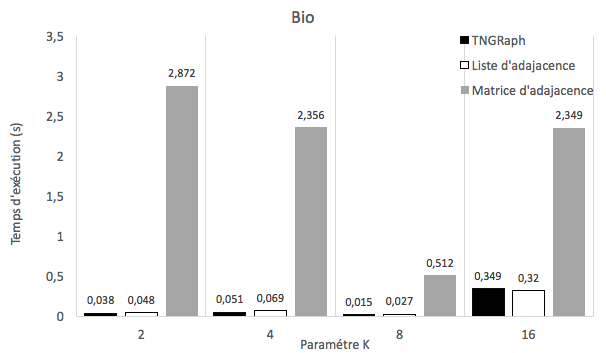
\includegraphics[scale=0.5]{ressources/image/Tests/rep-bio.png}}\hspace{3em}
			%\subfloat[{web-edu. \label{fig:testdom1}}]
			%{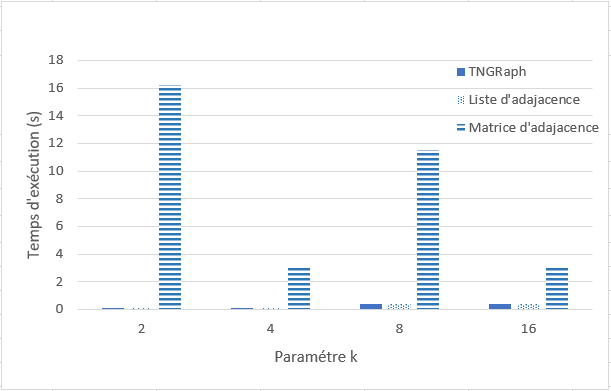
\includegraphics[scale=0.5]{ressources/image/Tests/rep-web-edu.png}}\hspace{3em}
			%\subfloat[{web-polblogs. \label{fig:testdom3}}]
			%{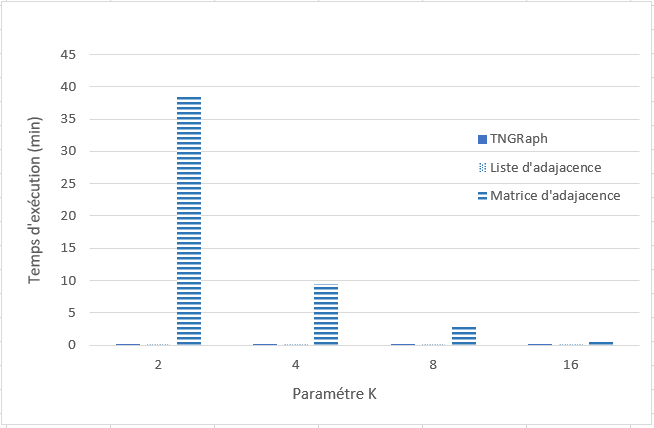
\includegraphics[scale=0.5]{ressources/image/Tests/rep-web-polblogs.png}}\hspace{3em}
			
			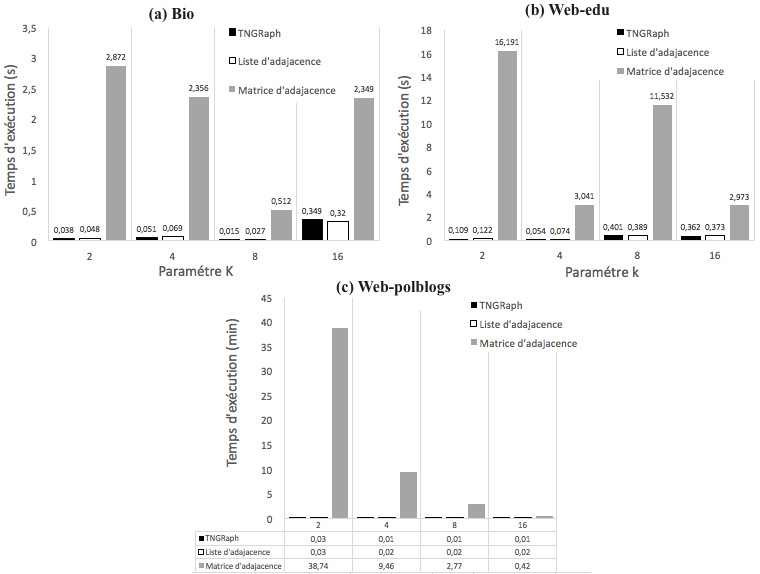
\includegraphics[scale=0.6]{ressources/image/Tests/tst.jpg}
			\caption{Résultats de tests du moteur $K^2$-Grace selon les différents types de représentations du graphe en entrée.}
			\label{fig:test-rep}
		\end{center}
	\end{figure}
			
Les graphiques de la figure  \ref{fig:test-rep} représentent la variation du temps d'exécution de la méthode $k^2$-trees selon les différentes représentations du graphe en entrée  sur trois graphes de tests : Bio, web-edu et web-polblogs. Cette compression a été effectuée avec un ordre initial et avec différentes valeurs de k. 

Nous constatons d'après les trois figures que l'utilisation des trois représentations donne des temps d'exécution totalement différents. Nous remarquons que si l'écart existant dans le temps d'exécution  entre l'utilisation de la matrice d'adjacence  et les deux autres structures peut être acceptable pour les petits graphes comme bio qui comptent 490 nœuds, il ne peut être toléré pour le cas des grands graphes comme web-edu et web-polblogs.
En effet, nous avons obtenu, dans le cas du graphe bio, un temps d'exécution entre 2 et 3 secondes dans le cas de l'utilisation de la matrice d'adjacence et un temps d'exécution entre 0,015 et 0,4 seconde dans les deux autres cas. Cependant, le cas du graphe web-polblogs donne un temps d'exécution de 38 minutes pour k=2 lorsque l'arbre est construit en utilisant la matrice d'adjacence et un temps d'exécution de 0,03 secondes dans le cas des deux autres structures. Cette différence est due au temps que prend la machine pour charger la matrice d'adjacence en mémoire centrale qui devient de plus en plus important lorsque la taille du graphe est grande. De ce fait, nous utiliserons uniquement la structure TNGraph pour la suite des tests.

			\subsection{Analyse de l'impact du paramètre k}
			Les figures \ref{fig:K2-paraK-NBbits} et \ref{fig:K2-paraK-Ratio} représentent respectivement l'évolution du nombre de bits par nœud et du ratio de compression en fonction des différentes valeurs du paramètre K. La compression a été appliquée sur différents graphes de test statiques issus de plusieurs domaines et avec différentes caractéristiques pour avoir une meilleure analyse. Les graphes utilisés dans ce test sont : bio, web-edu, web-polblogs, wiki et soc-Epinions. Cette compression a été effectuée avec un ordre initial et sans aucun pré-traitement.
%, avec comme paramètres :  (a voir aprés avec hafsa les noms des par).
 Nous avons varié le paramètre K entre 2 et 16.
			
\begin{figure}[H]
	\centering
	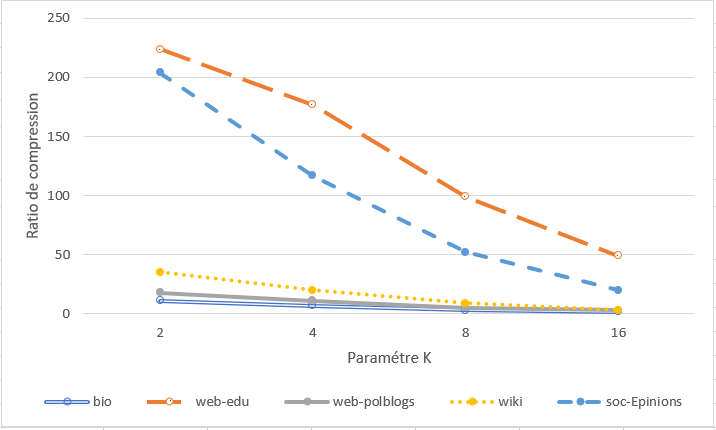
\includegraphics[scale=0.8]{ressources/image/Tests/K2-paraK-Ratio.png}
	
	\caption{Résultats de compression de $K^2$-Grace : Ratio de compression du moteur $K^2$-Grace en fonction du paramètre K (cas statique)}
	\label{fig:K2-paraK-Ratio}
\end{figure}

D'après les résultats obtenues dans la figure \ref{fig:K2-paraK-Ratio}, nous remarquons que le ratio de compression diminue quand k prend des valeurs plus grandes et atteint sa valeur minimale (exemple : 20 pour soc-Epinions) quand k=16. Ainsi, nous constatons que plus le k est petit plus le ratio de compression est optimal. En effet, pour des petites valeurs de k, l'arbre a plus de niveaux, mais il est moins large et le nombre de ses feuilles est plus petit (petites sous matrices finales) ce qui réduit la taille de l'arbre et donne une meilleur qualité de compression. Nous avons pu aussi confirmer cette hypothèse avec le nombre de bits par nœuds obtenu dans les différents cas et qui est représenté dans la figure \ref{fig:K2-paraK-NBbits}. Nous observons que le nombre de bits par nœud augmente de manière exponentielle en fonction de k et atteint sa valeur maximale (exemple 917 938 bits par nœud dans le cas du graphe wiki) quand k est à 16. Le nombre de bits augmente avec les grandes valeurs de k reflétant ainsi une augmentation dans la taille du graphe en sortie.

\begin{figure}[H]
	\centering
	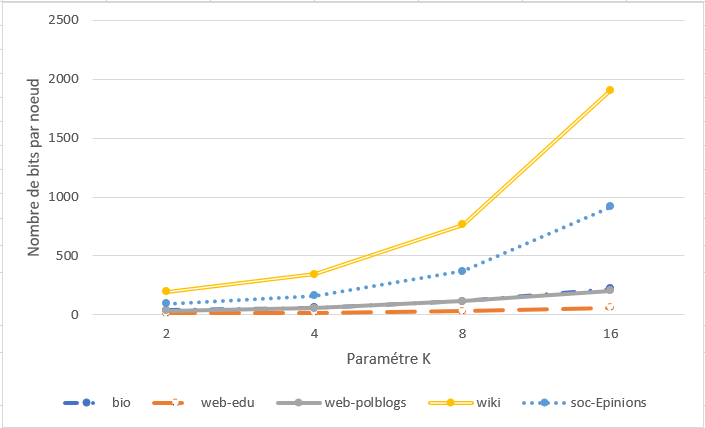
\includegraphics[scale=0.8]{ressources/image/Tests/K2-paraK-NBbits.png}
	
	\caption{Résultats de compression de $K^2$-Grace : Nombre de bits par nœuds en fonction du paramètre K}
	\label{fig:K2-paraK-NBbits}
\end{figure}		


Nous nous sommes aussi intéressées à l'étude de l'effet du paramètre k sur les performances de compression dans le cas des graphes dynamiques. Nous présentons dans la figure \ref{fig:K2-dyn-paraK-NBbits} les résultats obtenus pour ce type de graphes. Les graphes utilisés dans ce test sont : aves-weaver-social, reptilia-tortoise-network-bsv et reptilia-tortoise-network-fi. Ces graphes sont représentés avec leur captures initiales (sans aucun pré-traitement).

A partir de la figure \ref{fig:K2-dyn-paraK-NBbits}, nous remarquons une dégradation des performances dans le cas général. Cependant, nous obtenons les meilleurs performances pour k=8 dans le cas des deux graphes aves-weaver-social et reptilia-tortoise-network-bsv avec un 1,87 bits par nœud pour le premier graphe et 1,78 bits par nœud pour le deuxième graphe. De ce fait, l'hypothèse que nous avons avancée dans le cas des graphes statiques ne peut être généralisée dans le cas des graphes dynamiques où nous avons obtenu différentes valeurs optimales de k dans les différents graphes. 
\begin{figure}[H]
	\centering
	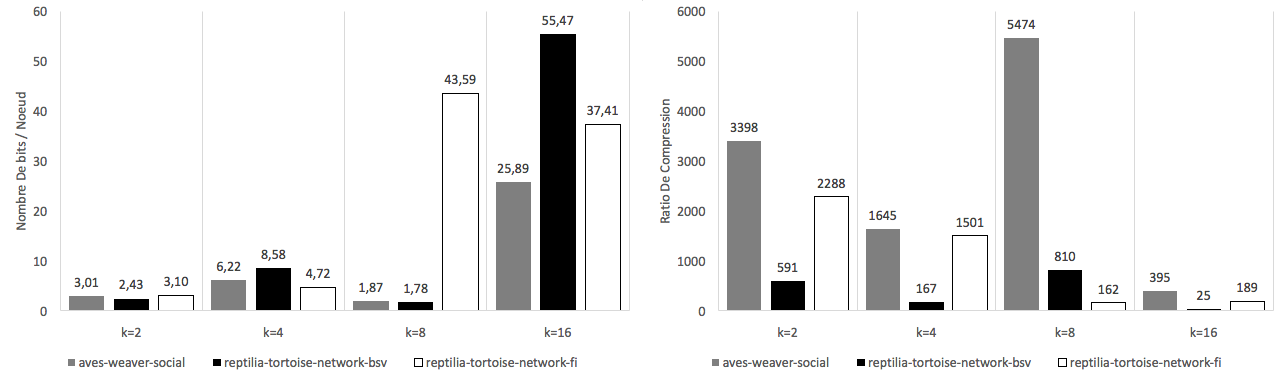
\includegraphics[scale=0.38]{ressources/image/ratioik2.png}
	
	\caption{Résultats de compression de $K^2$-Grace : Nombre de bits par nœud et Ratio de compression  du moteur en fonction du paramètre K (cas dynamique)}
	\label{fig:K2-dyn-paraK-NBbits}
\end{figure}	
	

La figure \ref{fig:K2-Texec} représente l'évolution du temps d'exécution en fonction du paramètre k. Dans le cas des graphes statiques, nous notons que le temps de compression varie de manière aléatoire et ne dépend pas de la valeur de k. En effet, dans le cas des graphes bio et soc-Epinions nous obtenons des temps d'exécution qui changent de manière aléatoire. Tant dis que dans le cas du graphe web-edu nous obtenons un temps d'exécution qui diminue en fonction de k contrairement au graphe wiki-Vote dans lequel le temps d'exécution  augmente en fonction du paramètre k. Dans le cas des graphes dynamiques, nous remarquons que le temps d'exécution diminue jusqu'à k=8 où il atteint sa valeur minimale pour k=8 et commence à augmenter à partir de cette valeur.


\begin{figure}[H]
	\centering
	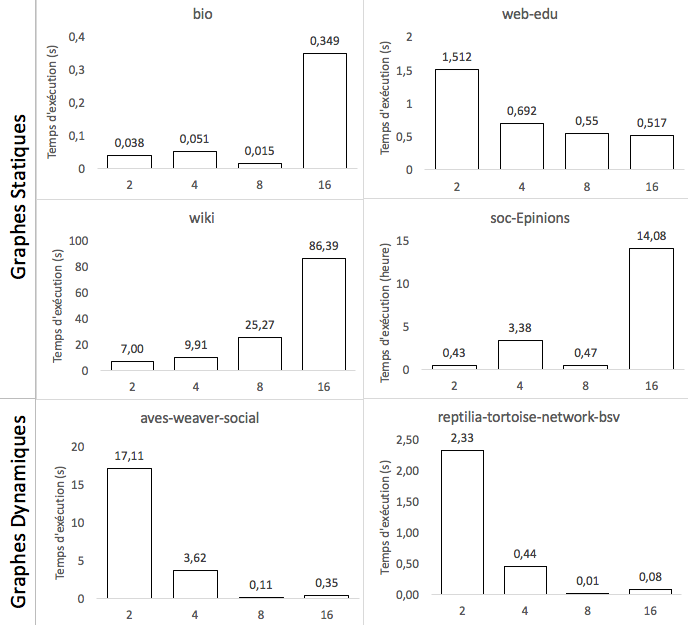
\includegraphics[scale=0.6]{ressources/image/Tests/K2-Texec.png}
	
	\caption{Résultats de compression de $K^2$-Grace : Temps de compression en fonction de K}
	\label{fig:K2-Texec}
\end{figure}


			
			
 \subsection{Étude de l'apport de la phase de pré-traitement }
 
 Durant cette partie de l'évaluation du moteur $k^2$-GraCE, nous nous focaliserons sur l'étude de l'effet de l'utilisation des techniques du module << pré-traitement >> du moteur $k^2$-GraCE. Nous commencerons par étudier l'effet des différents ordres des nœuds dans le cas des graphes orientés. Nous enchainerons par la mesure du gain apporté par la considération de la partie supérieure uniquement de la matrice d'adjacence dans la construction de l'arbre $k^2$-tree pour le cas des graphes non orientés. Finalement, nous présenterons les tests relatifs à l'utilisation d'une matrice de différence dans le cas des graphes dynamiques.
 			
\subsubsection{Étude de l'effet de l'ordre}

\begin{figure}[H]
	\centering
	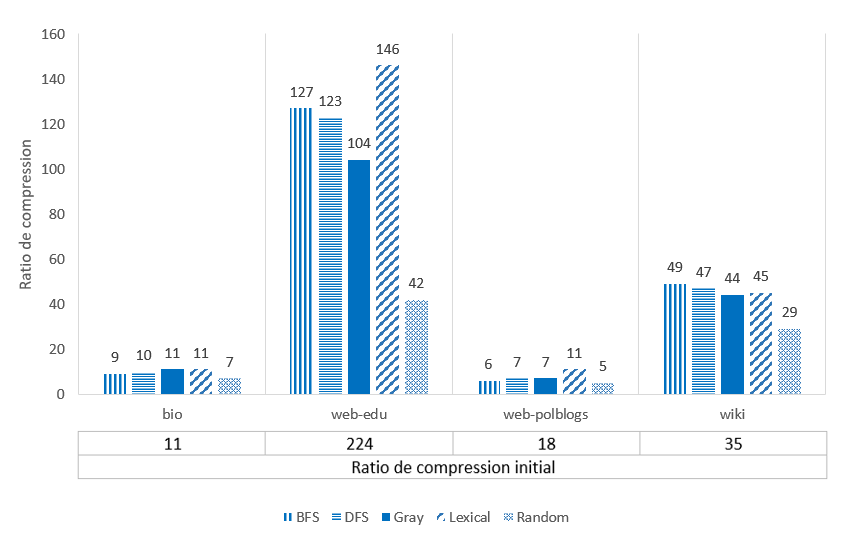
\includegraphics[scale=0.65]{ressources/image/Tests/k2-ordre.png}
	\caption{Résultats de compression de $K^2$-Grace :Ratio de compression selon l'ordre des nœuds}
	\label{fig:K2-ordre }
\end{figure}		

La figure \ref{fig:K2-ordre } représente l'évolution du ratio de compression du moteur $k^2$-Grace sur quatre graphes de test : bio, web-edu, web-polblogs et wiki. Cette compression a été effectuée en utilisant cinq ordres différents : BFS, DFS, Gray, Lexical et Random avec comme paramètre k=2. Nous remarquons que dans le cas des deux graphes web-edu et web-polblogs qui sont des graphes du web , nous avons obtenu une détérioration des performances de compression pour les différents ordres. Nous justifions cela par le fait que les arbres $k^2$-trees ont été au départ conçus pour exploiter les propriétés de l'ordre initial des nœuds dans la matrice d'adjacence. Cependant, nous remarquons que dans le cas du graphe wiki-Vote, qui est un graphe issu du domaine des réseaux sociaux, nous avons obtenu une amélioration du ratio initial d'un facteur de 1,4 avec les ordres : \gls{dfs}, \gls{bfs}, Gray et Lexical. Pour ce graphe, nous avons obtenu un ratio de compression optimal de 49 pour l'ordre BFS. Dans le cas du graphe bio, nous remarquons que seuls les ordres Lexical et gray ont permis de garder les même performances que l'ordre initial. Nous constatons donc que ces ordres donnent de bonnes performances avec les graphes qui ne sont pas issus du domaine du web. En effet, comme nous l'avons déjà noté s'ils ne permettent pas d'améliorer les performances ils ne les détériorent pas.


\subsubsection{Étude de l'effet de l'utilisation de la partie supérieure uniquement de la matrice d'adjacence}


Le tableau \ref{fig:tab-pret } donne les résultats de la compression du moteur $k^2$-Grace appliqué sans et avec pré-traitement sur des graphes non orientés avec un k=2 et un ordre initial des nœuds. Les graphes utilisés sont ChocWIki, ca-netscience, Caida. 
 

\begin{figure}[H]
	\centering
	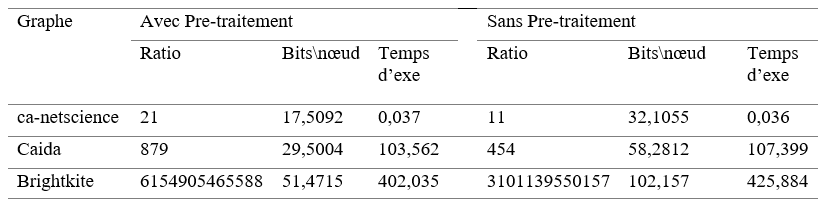
\includegraphics[scale=0.9]{ressources/image/Tests/tab-pret.png}
	\caption{Résultats de compression de $K^2$-Grace avec/sans pré-traitement (cas non orienté)}
	\label{fig:tab-pret }
\end{figure}

Nous observons que le ratio de compression et le nombre de bits par nœud sont nettement meilleurs avec le pré-traitement. Le pré-traitement appliqué sur le graphe non orienté maximise les zones vides dans la matrice d'adjacence en diminuant le nombre de 1 de moitié ce qui réduit la taille de l'arbre et produit une meilleure qualité de compression. Nous remarquons cela dans le ratio de compression qui double pour les trois graphes. Le temps d'exécution est presque le même dans les deux exécutions car nous construisons la matrice triangulaire supérieure au moment de la lecture directement. Le léger écart noté entre les deux exécutions est du aux comparaisons des indices sources et destinations effectuées pour construire la matrice. 

La figure \ref{fig:gain } présente le gain obtenu après l'application du pré-traitement sur les graphes non orientés, nous remarquons que le gain est aux alentours du double pour tous les graphes. Cela prouve que le pré-traitement améliore clairement la qualité de compression tout en offrant la possibilité d'extraire toutes les informations incluses dans le graphe original.

\begin{figure}[H]
	\centering
	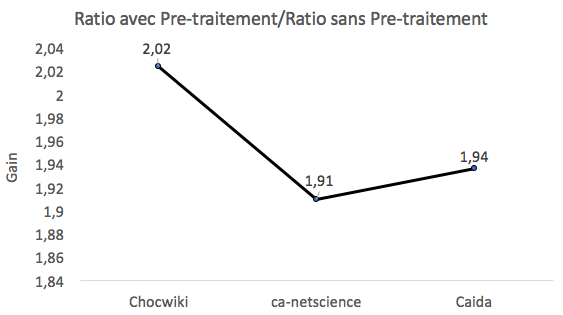
\includegraphics[scale=0.5]{ressources/image/gain.png}
	
	\caption{Gain de compression de $K^2$-Grace avec le pré-traitement}
	\label{fig:gain }
\end{figure}


\subsubsection{Étude de l'effet de l'utilisation d'une matrice de différence}

Dans cette partie, nous évaluerons l'effet de l'utilisation de la matrice de différence pour la construction de l'arbre sur les performances de compression. Comme les tests précédents ont montré  qu'il n'existe pas de valeur optimale pour k qui améliore ces derniers, nous effectuerons les tests de cette phase pour différentes valeurs de k. Le tableau de la figure \ref{res-dyn-tst} donne les valeurs des trois (03) métriques considérées en fonction des valeurs de k.


\begin{figure}[H]
	\centering
	\includegraphics[scale=0.48]{ressources/image/ik2.png}
	\caption{Résultats de compression de $K^2$-Grace avec/sans pré-traitement (cas dynamique)}
	\label{res-dyn-tst}
\end{figure}

Nous remarquons que nous obtenons dans tous les cas un temps d'exécution presque égal. Le léger écart noté dans le cas de l'utilisation du pré-traitement représente le temps nécessaire pour le calcule de la matrice de différence. 
Pour le graphe aves-weaver-social, nous remarquons que le ratio de compression (resp. le nombre de bits par nœud) diminue (resp. augmente) de moitié (resp. du double) pour toute les valeurs de k. Pour le deuxième graphe reptilia-tortoise-network-bsv, nous observons bien que les performances (ratio et nombre de bits par lien) restent les même dans les deux cas sans et avec pré-traitement. Tant dis que dans le cas du troisième graphe, nous remarquons que nous obtenons les mêmes performances pour k=2 et que nous perdons en performances quand  k prend des valeurs plus grandes. Pour mieux illustrer ces observations nous fournissons dans la figure \ref{perte } la courbe représentant le rapport entre le ratio de compression avant et après l'utilisation du pré-traitement. 


\begin{figure}[H]
	\centering
	\includegraphics[scale=0.5]{ressources/image/perteIk2.png}
	
	\caption{Ratio de avec pré-traitement/ Ratio de sans pré-traitement}
	\label{perte }
\end{figure}

Nous constatons donc que l'utilisation de ce module n'a pas amélioré les performances de compression dans le cas des trois graphes. Cela est du à la nature de leurs captures successives qui ne partagent presque aucun lien en commun engendrant ainsi soit la même matrice initiale ou une matrice de différence plus dense que celle du graphe original.



	\section{Évaluation du moteur P-GraCE}
	
	Nous évaluerons, dans cette partie, les méthodes de compression par extraction de motifs incluses dans le moteur P-GraCE. 
	Dans un premier temps, nous étudierons  le rondement de la méthode Subdue en fonction du niveau d'agrégation.  Nous enchainerons par la suite avec l'évaluation des performances de compression de \gls{vog} et \gls{ConDenSe} en fonction de la méthode de détection de communautés et de l'heuristique de sélection utilisés pour la compression. Nous aborderons par la suite l'approche basée sur les propriétés de la matrice d'adjacence représentée par la méthode \gls{gcupmt} où nous allons étudier l'influence du type et de la taille des motifs sur les mesures de performances.
	Finalement, nous présenterons les différents tests relatifs à la méthode de compression que nous avons proposée: \gls{ddsm} qui est destinée aux graphes dynamiques.
	\subsection{Évaluation de la méthode Subdue:}
	
  Durant cette section, nous considérons le cas des graphes non orientés et étiquetés. Nous évaluerons le rendement de compression de l'algorithme Subdue sur ces derniers tout en prêtant attention au temps d'exécution. La figure ci-dessous résume les résultats obtenus.
  

	\begin{figure}[H]
	
			
			\includegraphics[scale=0.37]{ressources/image/beam.png}
			
			\caption{Résultats des tests de Subdue.}
			\label{fig:test-beam}
	
	\end{figure}
	
	%%% Ajouter le tableau des resulats obtenus 
	
	  La figure \ref{fig:test-beam} illustre les résultats de tests obtenus pour différents graphes en fonction du nombre d'itérations de l'algorithme (le niveau d'agrégation). Nous constatons une amélioration du ratio de compression dans la majorité des cas. En contre partie, nous remarquons que le temps d'exécution  augmente surtout dans le cas des grands graphes (exemple du graphe credits). Le choix du nombre d'itérations (niveau de la hiérarchie d'agrégation) dépend des performances voulues. Cependant, nous pensons qu'un  nombre d'itération égale à 70 offre déjà un bon compromis entre le temps d'exécution et le ratio de compression.
	
	\subsection{Évaluation des techniques basées sur les méthodes de clustering (\gls{vog} et \gls{ConDenSe}) :}
	
	Dans cette partie, nous proposons de tester les méthodes de compression basées sur les techniques de clustering à savoir \gls{vog} et \gls{ConDenSe} en faisant varier différents paramètres. Dans un premier temps, nous fixerons  Slashburn comme méthode d'extraction de motifs et nous évaluerons les performances de compression obtenus avec la méthode de sélection \textit{TopK} en considérant à chaque fois une portion uniquement des structures découvertes (k=25\%,k= 33,33\%, k=50\%, k=100\%). Par la suite, nous étudierons l'effet  du choix de la méthode de sélection sur la qualité de compression en  utilisant la même méthode d'extraction de motifs. Finalement, nous analyserons l'effet de la méthode de clustering sur les résultats en fixant cette fois la méthode \textit{Step} comme méthode de sélection. Rappelons que la méthode \gls{vog} utilise SlashBurn comme méthode de clustering et les trois méthodes \textit{Plain}, \textit{TopK} et \gls{gnf} comme méthodes de sélection. De son coté \gls{ConDenSe} utilise plusieurs méthodes de clustering et la méthode \textit{Step} comme méthode de sélection.
	
	
		
		\subsubsection{Étude de l'influence du nombre de structures sélectionnées (\gls{vog}):}
	
		
		\begin{figure}[H]
	
			
			\includegraphics[scale=0.6]{ressources/image/vogStat.jpg}
			
			\caption{Résultats des tests de l'influence du nombre de structures sélectionnées.}
			\label{fig:test-select}
	
	\end{figure}
	
	La figure \ref{fig:test-select} illustre les mesures des trois métriques : ratio de compression, nombre de bits par nœud et le temps d'exécution en considérant différentes portions des sous-structures découvertes. Nous remarquons que le ratio de compression est presque équivalent pour les différentes valeurs de k. Cependant, nous observons bien que la considération de toutes les structures donne un meilleur ratio de compression de 1,06 pour chocWiki, de 1,23 pour netscience et de 1,03 pour le graphe Caida. Cette hypothèse peut être facilement confirmée avec le nombre de bits par noeud qui atteint sa valeur minimale avec la méthode \textit{Plain}. Quant au temps d'exécution, nous constatons  que la méthode \textit{Plain} offre toujours de meilleur performance. En effet, la méthode \textit{TopK} ordonne les sous-structures selon le gain d'encodage local avant la sélection engendrant ainsi un temps supplémentaire contrairement à la méthode \textit{plain} qui sélectionne toutes les sous-structures sans aucun ordre. Nous déduisons donc que \gls{vog} donne une meilleur qualité de compression avec Plain comme méthode de sélection.
		
		\subsubsection{Étude de l'influence de la méthode de sélection (\gls{vog} vs \gls{ConDenSe}):}
		
		\begin{figure}[H]
	
			
			\includegraphics[scale=0.7]{ressources/image/vogcond.jpg}
			
			\caption{Résultats des tests de l'influence de la méthode de sélection.}
			\label{fig:test-vogcond}
	
		\end{figure}
		
		Dans cette partie, nous présenterons les tests relatifs à l'utilisation de trois méthodes de sélection : Step, \gls{gnf} et \textit{Plain}. La figure \ref{fig:test-vogcond} résume les résultats obtenus sur  trois graphes non orientés statiques.
		
		Nous remarquons que la méthode Step donne de meilleur performances de compression avec un ratio maximale de 1,26 pour le graphe netscience qui compte 379 nœuds. En effet, si nous voulons classer ces méthodes de sélection selon les résultats du ratio et le nombre de bits par nœud nous obtenons le classement suivant: Step, \textit{Plain} et \gls{gnf} et ce pour tout les graphes utilisés dans ce test. Par contre, nous remarquons que la méthode Step donne un temps d'exécution qui est très élevé par rapport aux deux autres méthodes surtout dans le cas des grands graphes. Par exemple dans le cas du graphe Caida, nous avons obtenu un temps d'exécution de plus de quatre (04) heures avec la méthode Step  contre un temps d'exécution entre une (01) et deux (02) minutes pour les deux autres méthodes pour une amélioration de 0,04 dans le ratio de compression. Nous concluons que \gls{ConDenSe} avec son heuristique de sélection \textit{Step} donne de meilleures résultats de compression que la méthode \gls{vog} avec ses deux algorithmes de sélection \textit{Plain} et \gls{gnf} mais avec un temps d'exécution défavorable.
		
		\subsubsection{Étude de l'influence de la méthode de clustering sur les performance de \gls{ConDenSe}:}	
		
		\begin{figure}[H]
			\centering
			
			\includegraphics[scale=0.6]{ressources/image/clustmthd.png}
			
			\caption{Résultats des tests de l'influence de la méthode de clustering .}
			\label{fig:test-clustmtd}
	
	\end{figure}	
		
	
	Dans ce dernier test, nous nous sommes intéressées à voir le gain apporté par la méthode de clustering dans le ratio de compression. La figure \ref{fig:test-clustmtd} illustre les résultat obtenus. Nous avons considéré trois (03) méthodes de clustering: Slashburn, Spectral et K-cores. 
	
	Selon le graphe, les deux méthodes de compression Spectral et K-Cores donnent de meilleur résultat que SlaShburn pour les différents graphes. En effet, dans le cas du graphe ChocWiki la méthode spectrale donne le meilleur ratio (1,30). Tant dis que dans le cas des deux autres graphes, netscience et Caida, la méthode K-cores donne un meilleur ratio de 1,35 et 1,18 respectivement. Cependant, la combinaison des trois méthodes d'extraction de motifs donne une amélioration significative du ratio dans les trois graphes de test. 
Nous déduisons donc que \gls{ConDenSe} donne de très bon résultats quand les trois méthodes de détection de communautés sont appliquées ensemble.

	%Nous mesurons aussi le nombre de sous-strcuture dans chaque cas que nous accompagnons dans le tableau en dessous de la figure \ref{fig:test-clustmtd}. Nous remarquons que Slashburn donne dans tous les cas un nombre plus grands de sous-structures que les deux autres méthodes.
	
	
	
	\subsection{Étude de l'influence du type et de la taille des motifs dans la méthode \gls{gcupmt} :}
	
	Durant cette partie, nous présenterons les résultats obtenus lors de l'évaluation de l'extraction de motifs à partir de la matrice d'adjacence à travers la méthode \gls{gcupmt}. La figure \ref{fig:test-m} illustre l'évolution du ratio de compression en fonction de la taille du motif pour les trois types de motifs offerts par le moteur P-GracE.
		\begin{figure}[H]
		\begin{center}
		
			\includegraphics[scale=0.55]{ressources/image/m12.jpg}
			
			
			
			\caption{Le ratio de compression en fonction de la taille du motif.}
			\label{fig:test-m}
		\end{center}
	\end{figure}
	
	Dans le cas de la première et la troisième classe de motifs, nous remarquons une amélioration du ratio de compression lorsque leur taille prend des grandes valeurs. Cette observation est du au gain obtenu en remplaçant des motifs de taille $2^n$ bits par \textit{n} bits pour le premier type de motifs et \textit{n+1} bits pour le troisième, par exemple les motifs de taille 256bits seront remplacés par uniquement 8bits dans le cas de la classe (01) et par 9bits dans le cas de la classe (03). Pour la deuxième classe de motifs, le ratio de compression est resté presque constant pour différentes valeurs de la taille des motifs. Nous remarquons aussi que ce dernier est autour de 1 dans la majorité des cas, signifiant ainsi que la taille du graphe en sortie est presque équivalente à la taille du graphe initial. Ce résultat ne peut être obtenu que dans le cas où peu de motifs ont été trouvés dans la matrice d'adjacence. Nous constatons donc que les motifs de cette deuxième classe ne sont pas fréquents dans les matrices d'adjacence des graphes réels. 
	
	
	
	%\subsection{Évaluation de l'utilisation des méthodes de clustering :}
	
	
	
	
	\subsection{Évaluation de la méthode DDSM :}
	
	Nous présenterons dans cette partie, les tests relatifs à la méthode que nous avons proposée. Nous étudierons les performances obtenues en fonction du nombre de permutations utilisées dans le processus de découverte et d'étiquetage des sous-structures. 
\begin{figure}[H]
	
	\includegraphics[scale=0.4]{ressources/image/grDDSM.png}
	\label{fig:perte }
	\caption{Résultats de la méthode DDSM}
\end{figure}
		\begin{figure}[H]
		\begin{center}
		 \includegraphics[scale=0.45]{ressources/image/DDSM.jpg}
			
			
			\caption{Résultats des tests de la méthode DDSM.}
			\label{fig:test-ddsm}
		\end{center}
	\end{figure}
	
	Nous remarquons que la méthode proposée offre de très bon résultats par rapport au temps d'exécution qui ne dépasse pas une (01) seconde pour toutes les exécutions. Pour le ratio de compression, nous constatons une amélioration significative qui commence à se stabiliser à partir du moment où le nombre de permutations dépasse 50. 
	
	\begin{figure}[H]
		
		 \includegraphics[scale=0.38]{ressources/image/statDDSM.png}
			
			
			\caption{Statistique des différentes types de sous-structures découvertes}
			\label{fig:stat-DDSM}
		
	\end{figure}	
	
	Nous fournissons dans la figure \ref{fig:stat-DDSM} les différentes sous-structures découvertes pour un exemple d'exécution avec 50 permutations. Dans le cas du graphe Aves-weaver-social, nous remarquons que nous obtenons 30 sous-structures denses qui apparaissent de manière périodique et une seule sous-strcuture qui apparait de manière aléatoire. 
	Les sous-structures périodiques dans ce cas peuvent être interprétées comme des chasses d'animaux pour la nourriture.
	Dans les deux autres réseaux, nous remarquons aussi des sous-structures constantes qui représentent peut être des animaux appartenant à un même troupeau. 
	 Un autre type sont les sous-structures qui apparaissent dans une seule période représentant en générale le phénomène de couplage chez les animaux dans des périodes bien précises.
	
	\gls{ddsm} offre ainsi non pas uniquement la compression du graphe initial mais aussi la possibilité de l'analyser et d'interpréter les informations les plus pertinentes incluses dans ce dernier.
	
	\section{Comparaison entre les différentes méthodes:}
	
	Après avoir évaluer les différentes configurations possibles des deux moteurs : $k^2$-GraCE et P-GraCE, nous nous intéresserons dans cette partie à établir une étude comparative entre les méthodes implémentées dans les deux moteurs ainsi que les classes auxquelles elles appartiennent. Cette partie sera donc organisée en trois sous-sections, chacune englobe les méthodes de compression acceptant le même type de graphe en entrée.
	
	\subsection{Évaluation des méthodes destinées aux graphes orientés statiques :}
\begin{figure}[H]
		\begin{center}
		 \includegraphics[scale=0.4]{ressources/image/compNon.png}
			
			
			\caption{Comparaison entre les méthodes destinées aux graphes statiques orientés.}
			\label{fig:comp-dyn}
		\end{center}
	\end{figure}	
	
	Nous considérons dans cette partie les graphes orientés: bio, web-edu et web-polblogs, pour comparer entre trois méthodes de compression destinées pour ce type de graphe: $k^2$-GraCE pour les graphes orientés statique, la méthode \gls{dsm} et enfin la méthode \gls{gcupmt} basée sur la matrice d'adjacence. Nous utilisons pour cela deux métriques : le ratio de compression (figure à gauche) et le temps d'exécution (figure à droite). Nous remarquons que le moteur $k^2$-GraCE donne les meilleurs résultats en terme d'espace mémoire (le meilleur ratio). Cependant, il donne le plus grand temps d'exécution. Nous observons aussi que les deux autres méthodes donnent des résultats presque équivalents dans le des graphes bio et web-polblogs, et que la méthode \gls{dsm} donne un meilleur résultat dans le cas du graphe web-edu avec un ratio de 112 vs un ratio de 26 pour la méthode \gls{gcupmt}. 
	
	\subsection{Évaluation des méthodes destinées aux graphes non orientés statiques :}
	
	\begin{figure}[H]
	\centering
	\includegraphics[scale=0.65]{ressources/image/vogk2.png}
	\caption{Comparaison entre les méthodes destinées aux graphes statiques non orientés.}
	\label{fig:K2-vog}
\end{figure}	

	La figure \ref{fig:K2-vog}  donne les résultats de compression: ratio et temps de compression des deux méthodes de compression des moteur P-GraCE et $k^2$-GraCE dans le cas des graphes non orientés statiques. Nous utilisons dans ce test les graphes : ChocWiki, Caida et netscience. Pour le moteur $k^2$-GraCE, nous fixerons la valeur de k à 2 en considérant uniquement la partie supérieure de la matrice d'adjacence. Tant dis que pour le moteur P-GraCE, nous utiliserons \gls{ConDenSe} avec l'ensemble des méthodes de clustering pour l'extraction de motifs et la méthode \textit{step} pour la sélection.
	
	D'après l'illustration, nous observons que le ratio de compression du moteur $k^2$-GraCE  est nettement meilleur que celui du moteur P-GraCE. Nous citons l'exemple du graphe Caida qui comptent 26475 nœuds et 53381 arêtes où nous obtenons un ratio de compression de 879 dans $k^2$-GraCE contre un ratio de 1,40 avec le moteur P-GraCE. Quant au temps d'exécution, nous remarquons que le moteur $k^2$-GraCE est beaucoup plus rapide que P-GraCE surtout lorsque la taille du graphe devient grande (exemple du graphe Caida).
 
	
	\subsection{Évaluation des méthodes destinées aux graphes dynamiques :}
	
	Dans cette partie, nous allons comparer entre les deux méthodes de compression destinées aux graphes dynamiques qui sont incluses, la première dans le moteur $k^2$-GraCE et la deuxième dans le moteur P-GraCE consistant en un nouveau schéma de compression que nous proposons. La figure \ref{fig:comp-dyn} montre les résultats des deux méthodes de compression en choisissant les valeurs optimales de leurs paramètres.
	
	\begin{figure}[H]
		\begin{center}
		 \includegraphics[scale=0.4]{ressources/image/dynComp.png}
			
			
			\caption{Comparaison entre les méthodes destinées aux graphes dynamiques.}
			\label{fig:comp-dyn}
		\end{center}
	\end{figure}
	
	
	Nous remarquons que la ratio de compression est meilleur dans le moteur $k^2$-GraCE. En effet, la méthode \gls{ddsm} donne un ratio de compression très faible en la comparant avec le moteur $k^2$-GraCE (exemple: 3689 vs 129 pour le graphe aves-social-network). Cependant, nous observons bien que le temps d'exécution est nettement meilleur dans le cas de notre méthode. Nous rappelons aussi que notre méthode permet d'extraire les sous-graphes et les communautés les plus denses (les plus importantes) ainsi que leur comportement temporel avec un accès direct alors que le moteur $k^2$-GraCE nécessite un traitement supplémentaire qui peut être lourd dans le cas des grands graphes. 
	
	 
	
	\section{Synthèse des tests}
	
	A travers ce chapitre,  nous avons pu évaluer nos deux moteurs tout en étudiant l'effet de différentes configurations sur leurs performances. Des datasets de domaines hétérogènes ont été employés durant cette étape afin de déduire l'influence de ces derniers sur le choix de l'algorithme de compression. Nous avons opté pour trois métriques d'évaluation : ratio de compression, le nombre de bits par nœud et le temps d'exécution de l'algorithme de compression.
	
	Dans le cas du moteur $k^2$-GraCE, nous avons constaté que l'utilisation de la matrice d'adjacence pour la construction de l'arbre est trop couteuse en temps d'exécution. L'utilisation de la structure proposée dans la bibliothèque \gls{snap} donne des résultats nettement meilleurs pour cette métrique. Nous avons aussi observé que le choix du paramètre k influe fortement sur les performances de la compression. Selon les résultats obtenus, la valeur optimale dans le cas statique est bien k=2. De plus, nous avons constaté que l'utilisation d'un ré-ordonnancement des nœuds n'est intéressant que dans le cas des graphes autres que les graphes du web où nous avons obtenu une amélioration du ratio de compression d'un facteur de 1,4 dans le cas du graphe wiki-Vote. La généralisation  proposée pour le cas des graphes statiques non orientés permet de doubler le ratio de compression améliorant ainsi la qualité de la compression. D'autre part, nous avons remarqué que l'utilisation du graphe original dans le cas dynamique donne de meilleurs résultats. En effet, nous avons constaté que l'utilisation de la matrice de différence n'est bénéfique que dans le cas où les captures possèdent un degré élevé de ressemblance des liens, ce qui n'est généralement pas le cas dans les graphes réels.
	
	Le deuxième moteur, P-GraCE, permet de compresser le graphe en entrée avec ses sous-structures les plus importantes. Les tests ont montré qu'il n'est pas intéressant d'utiliser le deuxième type de motifs dans la méthode  basée sur les propriétés de la matrice d'adjacence (\gls{gcupmt}) car il est peu fréquent dans les graphes réels. Pour la méthode Subdue, nous avons bien remarqué que le niveau d'agrégation doit être choisi d'une manière qui assure un compromis entre le temps d'exécution et le ratio de compression. L'évaluation des méthodes basées sur les techniques de clustering, à savoir \gls{vog} et \gls{ConDenSe}, a montré que l'utilisation de la méthode \gls{ConDenSe} donne les meilleurs performances avec : (1) \textit{Step} comme méthode de sélection, (2) l'ensemble des trois méthodes de clustering pour l'extraction de motifs. Finalement, l'évaluation de la méthode \gls{ddsm} que nous proposons a montré qu'elle donne des résultats compétitifs en terme de temps de compression. Certes, le moteur $k^2$-GraCE offre un meilleur ratio dans le cas dynamique mais il n'offre pas les mêmes avantages que la méthode que nous proposons. En effet, le résultat obtenu par \gls{ddsm} permet une analyse très rapide des communautés et leurs comportements temporels.
	
	La comparaison entre les deux moteurs nous a amené à déduire que l'utilisation du moteur $k^2$-GraCE est meilleur dans le cas où le but est de diminuer la taille du graphe uniquement. Cependant, le moteur P-GraCE permet d'avoir des informations interprétables qui aident dans l'analyse du graphe car il permet de synthétiser l'information incluse dans le graphe initial sous forme des sous-structures les plus pertinentes.
	
	
	
	
	
	
	
	
	
	
	
	
	
	
	
	
	
	
	
	
	
	
	
	
	
	
	




%\chapter{Conclusion Générale}
\newpage
\Huge{ 
			\textbf {Conclusion générale}} \\[0.5in]
			\addcontentsline{toc}{chapter}{\numberline{}Introduction générale}
			\normalsize
De nos jours, les graphes sont omniprésents. Cependant, leur taille présente un obstacle presque insurmontable à la compréhension du caractère essentiel des données. D'où la nécessité de la compression qui permet de réduire la taille des graphes tout en gardant le caractère utile de l'information incluse dans ces derniers.\\

Dans notre travail, nous nous sommes focalisées  sur les méthodes de compression basées sur l'extraction de motifs et celles basées sur les arbres $k^2$-trees. Dans un premier temps, nous avons étudié les différentes méthodes et techniques s'inscrivant dans les deux classes ainsi que leurs différentes classifications existantes dans la littérature. Cette étude nous a initié au domaine de compression et nous a permis de mieux comprendre l'approche théorique de chaque classe. Suite à cela, nous avons proposé une nouvelle classification consistant en une rectification d'une ancienne classification proposée dans un Master précédent \citep{master2017}. Nous nous sommes basées pour cela sur le principe de fonctionnement et les fondements théoriques de ces méthodes. Nous avons conclu cette partie en établissant une étude comparative au sein d'une même classe et entre les deux classes en considérant différents critères: type de graphe en entrée, type de compression, .... \\

La deuxième partie de notre travail consiste en l'implémentation d'une méthode de chaque classe que nous  avons proposées dans la première étape dans le but de les réunir dans une même plateforme et d'établir une comparaison plus objective entre ces techniques. De ce fait, nous avons proposé deux moteurs de compression de graphe (un moteur par classe). Le premier moteur $k^2$-GraCE exploite les propriétés de la matrice d'adjacence pour compresser le graphe. Il supporte trois types de graphe : graphes statiques orientés, graphes statiques non orientés et les graphes dynamiques. Nous l'avons doté d'une phase de pré-traitement qui permet d'exploiter davantage les caractéristiques des graphes. Le deuxième moteur P-GraCE quant à lui supporte trois types de graphe : graphes orientés statiques, graphes non orientés statiques et finalement les graphes étiquetés. Il englobe quatre approches de compression : une approche basée sur le beam search, une approche basée sur les méthodes de clustering, une approche basée sur le MinHashing et une approche basée sur l'extraction de motifs à partir de la matrice d'adjacence. Nous avons aussi proposé une nouvelle méthode de compression s'intitulant DDSM destinée pour les graphes dynamiques et permettant de fournir une compression interprétable du graphe initial. \\

La dernière étape de notre projet représente une étape d'évaluation des deux moteurs de compression ainsi que la méthode que nous avons proposée. Nous avons utilisé pour cela des graphes réels issus de domaines différents ainsi que trois métriques d'évaluation : le ratio de compression, le nombre de bits par nœud et le temps d'exécution. Dans le cas du moteur $k^2$-GraCE, nous avons montré que l'utilisation de la matrice d'adjacence dégrade les performances en terme de temps d'exécution et que l'utilisation de la liste d'adjacence ou la structure de la bibliothèque \gls{snap} est meilleur. Pour le module de pré-traitement de ce moteur, nous avons constaté que  l'utilisation d'algorithme de ré-ordonnancement  ne donne une amélioration que dans le cas des graphes qui ne sont pas issus du domaine du web. Nous avons aussi obtenu une amélioration d'un facteur de 2 du ratio de compression lorsque la partie supérieure uniquement de la matrice est considérée. Le meilleur ratio obtenu pour ce moteur est de 5474 dans le cas du graphe Retilia--toroise-network-bsv qui est un graphe dynamique.
Pour le deuxième moteur P-GracE, les tests ont montré que, dans le cas de la méthode basée sur les propriétés de la matrice d'adjacence, les motifs de classe une (01) ou de classe trois (03) sont plus intéressants. Nous avons aussi constaté que l'approche basée sur les méthodes de clustering produit une meilleur compression lors de l'utilisation des trois méthodes de clustering ensembles comme méthode d'extraction de motifs et la méthode \textit{Step} comme méthode de sélection. Concernant la méthode que nous avons proposée, nous avons obtenu un ratio de compression qui se stabilise à partir de 50 permutations avec un temps de compression compétitif.  
La comparaison entre les deux moteurs a montré que le moteur $k^2$-GraCE donne des résultat nettement meilleur que le moteur P-GraCE en terme de taux de compression. Cependant, le moteur P-GraCE offre une compression dans un temps meilleur tout en produisant une compression qui facilite l'analyse et la compréhension du graphe initial à travers ses sous-structures les plus importantes ayant généralement une interprétation selon le domaine d'application.  \\
	
	
Comme perspective à ce travail, nous aimerions bien tester nos deux moteurs avec des graphes encore plus larges pour pouvoir les évaluer davantage. Nous voudrons aussi tester notre méthode contre les méthodes existantes dans la littérature, notamment TimeCrunch \citep{shah2015timecrunch}, sur les mêmes graphes afin de mieux comparer et situer notre contribution dans la littérature.






\pagestyle{plain}
\newpage

\begin{appendix}


\chapter{Extraction de voisins dans un arbre $k^2$-tree}
    \label{k2_annexe}
La compression par les arbres $k^2$-trees a connue un large succès dans la communauté scientifique. L'une des causes les plus importantes qui ont favorisé cela est qu'elle permet d'extraire le voisinage des nœuds sans reconstitution du graphe initiale. Cette partie se veut une explication des deux algorithmes d'extraction de voisins directes et inverses. 

Comme nous l'avons déjà expliqué dans la section \ref{k2} de la partie conception   du moteur $k^2$-GraCE, les arbres $k^2$-tree sont représentés en mémoire à l'aide de deux chaines binaires, T et L, qui regroupe le contenue de l'arbre de haut vers le bas et de la gauche vers la droite. Nous fournissons ci-après les algorithmes d'extraction de voisinage \citep{brisaboa2009k}.



\begin{multicols}{2}

\begin{algorithm}[H]
					\label{alg:Direct}
					\caption{Direct}
					\textbf{Entrée :}
						\begin{itemize}[label=$\bullet$]
							\item n : la taille de la sous-matrice
							\item p : l'indice de la ligne 
							\item q : l'indice de la colonne
							\item x : l'indice dans l'arbre
						\end{itemize}
					\textbf{Sortie :} affichage des voisins Directes\\							\noindent\rule{\textwidth}{1pt}
						
						
				\begin{algorithmic} [1]
					\IF {x $\geqslant$ |T|}
						\IF { L[x-|T|] =1 }
							\STATE afficher q
						\ENDIF
					\ELSE
						\IF { x = -1 ou T[x]=1  }
							\STATE y = rank(T,x)*$k^2$ + p/(n/k)
							\FOR{ j =0 ... k-1}
								\STATE Direct(n/k,p mod(n/k),q+ j*(n/k),y+j)
							\ENDFOR
						\ENDIF
					\ENDIF 
					
					
				\end{algorithmic}
			\end{algorithm}


 
\columnbreak
 
\begin{algorithm}[H]
					\label{alg:Inverse}
					\caption{Inverse}
					\textbf{Entrée :}
						\begin{itemize}[label=$\bullet$]
							\item n : la taille de la sous-matrice
							\item q : l'indice de la colonne
							\item p : l'indice de la ligne 
							\item x : l'indice dans l'arbre
						\end{itemize}
					\textbf{Sortie :} affichage des voisins Inverses\\							\noindent\rule{\textwidth}{1pt}
						
						
				\begin{algorithmic} [1]
					\IF {x $\geqslant$ |T|}
						\IF { L[x-|T|] =1 }
							\STATE afficher p
						\ENDIF
					\ELSE
						\IF { x = -1 ou T[x]=1  }
							\STATE y = rank(T,x)*$k^2$ + q/(n/k)
							\FOR{ j =0 ... k-1}
								\STATE Inverse(n/k,q mod(n/k),p+ j*(n/k),y+j*k)
							\ENDFOR
						\ENDIF
					\ENDIF 
					
					
				\end{algorithmic}
			\end{algorithm}
			
\end{multicols}

\chapter{Description des graphes de test}
 \label{tableau des graphes de test}
 \begin{table}[H]
 \begin{tabular}{|C{5cm}|C{4.5cm}|C{4.5cm}|}
		\hline
		\multirow{2}{*}{Graphe de test} & \multicolumn{2}{c|}{Caractéristiques}  \\ \cline{2-3}
				&  Nombre de nœuds & Nombre de liens  \\ \hline	 \hline	
 
eu-2005 & 862 milles de nœuds & 19M de liens \\ \hline
Cond-mat & 36 milles de nœuds & 171 milles de liens \\ \hline
CommNet & \multicolumn{2}{c|}{taille : 225.9MB} \\ \hline
SalesDay & 1 milles de nœuds & \\ \hline
Movielens10M & 10 milles de nœuds & 10M de liens \\ \hline
ASOregon &  13 milles nœuds & 37 milles liens \\ \hline
 Enron &  80 milles nœuds& 288 milles liens \\ \hline
 uk-2002 & 18 milles nœuds & 298 milles liens \\ \hline
 graphe test de GCUPMT &  8 192 milles nœuds & \\ \hline
 Composante chimique &  21 étiquettes & 422 transactions \\ \hline
 NotreDame &  325 milles de nœuds & 1M de liens \\ \hline



\end{tabular}
									\caption{Graphes de test}									\label{comgen}

 								\end{table}
\end{appendix}






\newpage


\chapter{Algorithmes des méthodes de clustering}

\label{SlashBurn}

\begin{algorithm}[H]
					\label{alg:SlashBurn}
					\caption{SlashBurn}
					\textbf{Entrée :}
						\begin{itemize}[label=$\bullet$]
							\item G(V,E) : Graphe non orienté 
							\item n : nombre de nœuds dans le graphe 
							
						\end{itemize}
					\textbf{Sortie :} ensemble de structures\\							\noindent\rule{\textwidth}{1pt}
						
						
				\begin{algorithmic} [1]
				 \STATE 
				 \STATE D = [] //tableau de degré
				 \STATE GCC : un graph				 				 \FOR{ i=0 .. n-1}
				 \STATE D[i] = \textbf{Degré}(i)
				 \ENDFOR
				 
					\STATE hub = \{ i | max(D[i])\}
					
					\STATE spokes = \{ i | min(D[i])\} //nœuds isolés 
					\STATE GCC = G(V) - \{$e_{hub}$\} - \{$e_{spokes}$\}
					
					
				
				\STATE SlashBurn(GCC, Taille du GCC)  
				\end{algorithmic}
			\end{algorithm}

\newpage

\label{KCBC}


\begin{algorithm}[H]
					\label{alg:KCBC}
					\caption{KCBC}
					\textbf{Entrée :}
						\begin{itemize}[label=$\bullet$]
							\item G : Graphe non orienté
							\item n : nombre de nœuds dans le graphe 
							
						\end{itemize}
					\textbf{Sortie :} ensemble de structures\\							\noindent\rule{\textwidth}{1pt}
						
						
				\begin{algorithmic} [1]
				\STATE Degré = 	\lbrack \rbrack
				\STATE F = G
				\STATE stop = VRAI
				\STATE structure = \{\}
				\STATE //étape 1 : Calculer le degré de chaque nœud
					\FOR{ i =0 ... n-1}
					  \STATE Degré \lbrack i \rbrack = $\textbf{Deg}_G$(i)
					  \ENDFOR
					  \STATE $k_{max}$ = k
						\WHILE { $k_{max}$ > 1 and and stop = VRAI }
						\STATE //étape 2 : Décomposition du graphe avec $k_{max}$
						\STATE F = G
						\FOR{ x =0 ... n-1}
							\IF { $\textbf{DEG}_F$(x) < $k_{max}$}
							\STATE $\textbf{Supprimer}_F$(x) 
							\ENDIF
							
						\ENDFOR
						
						\IF { F = {} }
							\STATE stop = FAUX
						
					\ELSE
						\STATE $k_{max}$ = $k_{max}$ - 1
					\ENDIF
					\ENDWHILE 
					
					
					\STATE //étape 3 : Identification des structures 
					
					\STATE structure = structure $\cup$ \{ composants connexes $ \in $ F \}
					 
					 \STATE //étape 4 : Suppression des arêtes entre structures
					 \FOR{ $struct_i$, $struct_j$ $\in$ structure } 
					 \STATE $\textbf{supprimerArête}_F$($struct_i \cap struct_j$)   
					 \ENDFOR
				\end{algorithmic}
			\end{algorithm}

\newpage
\label{Louvain}


\begin{algorithm}[H]
					\label{alg:Lovain}
					\caption{Louvain}
					\textbf{Entrée :}
						\begin{itemize}[label=$\bullet$]
							\item G(V,E) : Graphe non orienté pondéré
							\item n : nombre de nœuds dans le graphe 
							
						\end{itemize}
					\textbf{Sortie :} ensemble de structures\\							\noindent\rule{\textwidth}{1pt}
						
						
				\begin{algorithmic} [1]
				 \STATE //Phase 1
				 \STATE $C$ = \{\{$v_i$ \} | $v_i \in G(V)$ \}
				 \REPEAT
				 \FOR{ $v_i \in C_x$ and $v_j \in C_y$ and $(v_i,v_j) \in G(E)$}
					\STATE H = \{ $\Delta Q_i(C_x,C_y)$ | $C_x,C_y \in C$ \}
					\IF{\textit{max}$\Delta Q_i(C_x,C_y)$ > 0}
					\STATE $C_y$ = $C_y \cup \{v_i\}$
					\STATE $C_x$ = $C_x$ - \{$v_i$\}
					 \ENDIF
					  \ENDFOR
					  \STATE //Phase 2
					 \STATE V' = \{ $C_x$ | $C_x \in C$ \}
					  \STATE E' = \{ $\sum \frac{(v_i,v_j)}{1}$ | $v_i \in C_x$ | $v_j \in C_y$ | $e_{i,j} \in G(E)$ \}
					 \STATE G = G'(V',E')
					  \UNTIL{aucune amélioration possible}
				\STATE ensemble de structures = \{ $v_i$ | $v_i \in G$ \} 	   
				\end{algorithmic}
			\end{algorithm}



\bibliographystyle{apalike}
\bibliography{Bibliographie}

\end{document}

%\renewcommand{\thefigure}{\arabic{figure}}
%\setcounter{figure}{0}
%\begin{figure}[H]
%	\centering
%	\includegraphics[scale=1]{ressources/image/LAAS-2016.jpg}
%	\label{fig:figure1}
%	\caption{This is a teste of figure}
	
%\end{figure}








